%%%%%%%%%%%%%%%%%%%%%%%%%%%%%%%%%%%%%%%%%
% Masters/Doctoral Thesis
% LaTeX Template
% Version 2.5 (27/8/17)
%
% This template was downloaded from:
% http://www.LaTeXTemplates.com
%
% Version 2.x major modifications by:
% Vel (vel@latextemplates.com)
%
% This template is based on a template by:
% Steve Gunn (http://users.ecs.soton.ac.uk/srg/softwaretools/document/templates/)
% Sunil Patel (http://www.sunilpatel.co.uk/thesis-template/)
%
% Template license:
% CC BY-NC-SA 3.0 (http://creativecommons.org/licenses/by-nc-sa/3.0/)
%
%%%%%%%%%%%%%%%%%%%%%%%%%%%%%%%%%%%%%%%%%


%----------------------------------------------------------------------------------------
%	PACKAGES AND OTHER DOCUMENT CONFIGURATIONS
%----------------------------------------------------------------------------------------

\documentclass[
11pt,                   % The default document font size, options: 10pt, 11pt, 12pt
%oneside,               % Two side (alternating margins) by default, uncomment to switch to one side
english,                % The language option
singlespacing,          % Single line spacing, alternatives: onehalfspacing or doublespacing
%draft,                 % Uncomment to enable draft mode (no pictures, no links, overfull hboxes indicated)
%nolistspacing,         % If the document is onehalfspacing or doublespacing, uncomment this to set spacing in lists to single
%liststotoc,            % Uncomment to add the list of figures/tables/etc to the table of contents
%toctotoc,              % Uncomment to add the main table of contents to the table of contents
%parskip,               % Uncomment to add space between paragraphs
%nohyperref,            % Uncomment to not load the hyperref package
headsepline,            % Uncomment to get a line under the header
%chapterinoneline,      % Uncomment to place the chapter title next to the number on one line
%consistentlayout,      % Uncomment to match to default the layout of the declaration, abstract...
]{MastersDoctoralThesis}

\usepackage[utf8]{inputenc}   % Required for inputting international characters
\usepackage[T1]{fontenc}      % Output font encoding for international characters
\usepackage{mathpazo}         % Use the Palatino font by default
\usepackage{mathtools}        % it also loads amsmath
\usepackage{amssymb}          % it also loads amsfonts
\usepackage{bm}               % bold Greek letters
\usepackage{xfrac}            % slanted frac
\usepackage{subcaption}       % sub-figures
\usepackage{fix-cm}           % arbitrary font size
\usepackage{float}            % placing figures
\usepackage{multirow}         % join cells at different rows of a table
\usepackage{makecell}         % makecell command, allow line break inside a cell of a table
\usepackage[backend=bibtex8,style=numeric-comp,giveninits=true,natbib=true,maxbibnames=9,maxcitenames=7]{biblatex}

\addbibresource{../bibliography/sw.bib}

\usepackage[autostyle=true]{csquotes} % Language-dependent quotes in the bibliography

%----------------------------------------------------------------------------------------
%	SECTIONING DEFINITIONS
%----------------------------------------------------------------------------------------

\setcounter{tocdepth}{3}
\setcounter{secnumdepth}{3}

%----------------------------------------------------------------------------------------
%	CUSTOM DEFINITIONS
%----------------------------------------------------------------------------------------

\newcommand{\pder}[2]{\frac{\partial#1}{\partial#2}}
\newcommand*{\ppder}[2]{\frac{\partial^2#1}{\partial#2^2}}
\newcommand*{\abs}[1]{\lvert#1\rvert}
\newcommand*{\norm}[1]{\lVert#1\rVert}
\newcommand*{\defeq}{\mathrel{\vcenter{\baselineskip0.5ex\lineskiplimit0pt\hbox{\scriptsize.}\hbox{\scriptsize.}}}=}
\newcommand*{\ldbrace}{\{\mskip-5mu\{} % left double curly braces
\newcommand*{\rdbrace}{\}\mskip-5mu\}} % right double curly braces


%----------------------------------------------------------------------------------------
%	MARGIN SETTINGS
%----------------------------------------------------------------------------------------

\geometry{
	paper=a4paper, % Change to letterpaper for US letter
	inner=2.5cm, % Inner margin
	outer=3.8cm, % Outer margin
	bindingoffset=.5cm, % Binding offset
	top=1.5cm, % Top margin
	bottom=1.5cm, % Bottom margin
	%showframe, % Uncomment to show how the type block is set on the page
}


%----------------------------------------------------------------------------------------
%	THESIS INFORMATION
%----------------------------------------------------------------------------------------

\date{June 28, 2022}
\thesistitle{Coupling shallow water models with three-dimensional models for the study of fluid-structure interaction problems using the particle finite element method} % print it with \ttitle
\supervisor{Dr. Eugenio \textsc{Oñate}} % print it with \supname
\cosupervisor{Dr. Ignasi \textsc{de-Pouplana}} % print it with \cosupname
\examiner{} % this is not currently used, print it with \examname
\degree{Civil Engineering Ph. D.} % print it with \degreename
\author{Miguel \textsc{Masó}} % print it with \authorname
\addresses{} % this is not currently used, print it with \addressname
\subject{Civil Engineering} % this is not currently used, print it with \subjectname
\keywords{} % this is not currently used, print it with \keywordnames
\university{\href{http://www.upc.edu}{Universitat Politècnica de Catalunya Barcelona Tech}} % print it with \univname
\department{\href{http://www.deca.upc.edu}{Department of Civil and Environmental Engineering}} % print it with \deptname
\group{\href{http://www.cimne.com}{International Centre for Numerical Methods in Engineering}} % print it with \groupname
\faculty{\href{http://www.etseccpb.upc.edu}{Barcelona School of Civil Engineering}} % print it with \facname

\colorlet{wrmBlue}{blue!30!black}
\colorlet{wrmGreen}{green!30!black}
\AtBeginDocument{
\hypersetup{pdftitle=\ttitle} % Set the PDF's title to your title
\hypersetup{pdfauthor=\authorname} % Set the PDF's author to your name
\hypersetup{pdfkeywords=\keywordnames} % Set the PDF's keywords to your keywords
\hypersetup{linkcolor=wrmBlue}
\hypersetup{citecolor=wrmGreen}
}



%%%%%%%%%%%%%%%%%%%%%%%%%%%%%%%%%%%%%%%%%%%%%%%%%%%%%%%%%%%%%%%%%%%%%%%%%%%%%%%%%%%%%%%%%
%%%%%%%%%%%%%%%%%%%%%%%%%%%%%%%%%%%%%%%%%%%%%%%%%%%%%%%%%%%%%%%%%%%%%%%%%%%%%%%%%%%%%%%%%
%%%%%%%%%%%%%%%%%%%%%%%%%%%%%%%%%%%%%%%%%%%%%%%%%%%%%%%%%%%%%%%%%%%%%%%%%%%%%%%%%%%%%%%%%

% \includeonly{chapters/equations, chapters/eulerian_sw, chapters/eulerian_bsq}

%%%%%%%%%%%%%%%%%%%%%%%%%%%%%%%%%%%%%%%%%%%%%%%%%%%%%%%%%%%%%%%%%%%%%%%%%%%%%%%%%%%%%%%%%
%%%%%%%%%%%%%%%%%%%%%%%%%%%%%%%%%%%%%%%%%%%%%%%%%%%%%%%%%%%%%%%%%%%%%%%%%%%%%%%%%%%%%%%%%
%%%%%%%%%%%%%%%%%%%%%%%%%%%%%%%%%%%%%%%%%%%%%%%%%%%%%%%%%%%%%%%%%%%%%%%%%%%%%%%%%%%%%%%%%



\begin{document}

\frontmatter % Use roman page numbering style (i, ii, iii, iv...) for the pre-content pages

\pagestyle{plain} % Default to the plain heading style until the thesis style is called for the body content


%----------------------------------------------------------------------------------------
%	TITLE PAGE
%----------------------------------------------------------------------------------------

\begin{titlepage}
\begin{center}

\vspace*{.06\textheight}
{\scshape\LARGE \univname\par}\vspace{1.5cm} % University name
\textsc{\Large Doctoral Thesis}\\[0.5cm] % Thesis type

\HRule \\[0.4cm] % Horizontal line
{\huge \bfseries \ttitle\par}\vspace{0.4cm} % Thesis title
\HRule \\[1.5cm] % Horizontal line
 
\begin{minipage}[t]{0.4\textwidth}
\begin{flushleft} \large
\emph{Author:}\\
\href{https://directori.upc.edu/directori/dadesPersona.jsp?id=1115243}{\authorname}
\end{flushleft}
\end{minipage}
\begin{minipage}[t]{0.4\textwidth}
\begin{flushright} \large
\emph{Supervisors:} \\
\href{http://www.cimne.com/eo}{\supname} \\
\href{https://www.cimne.com/1898/2181/people/directory}{\cosupname}
\end{flushright}
\end{minipage}\\[.3cm]
 
\vfill

\large \textit{A thesis submitted in fulfillment of the requirements\\ for the degree of \degreename}\\[0.3cm] % University requirement text
\textit{in the}\\[0.3cm]
\groupname\\\deptname\\[.3cm] % Research group name and department name
 
\vfill

{\large \today}\\[1cm]
\href{https://camins.upc.edu/}{

\includegraphics[width=.6\textwidth]{img/logo_caminos.png}
}
\vfill
\end{center}
\end{titlepage}


%----------------------------------------------------------------------------------------
%	DECLARATION PAGE
%----------------------------------------------------------------------------------------

% \begin{declaration}
% \addchaptertocentry{\authorshipname} % Add the declaration to the table of contents
% \noindent I, \authorname, declare that this thesis titled, \enquote{\ttitle} and the work presented in it are my own. I confirm that:

% \begin{itemize} 
% \item This work was done wholly or mainly while in candidature for a research degree at this University.
% \item Where any part of this thesis has previously been submitted for a degree or any other qualification at this University or any other institution, this has been clearly stated.
% \item Where I have consulted the published work of others, this is always clearly attributed.
% \item Where I have quoted from the work of others, the source is always given. With the exception of such quotations, this thesis is entirely my own work.
% \item I have acknowledged all main sources of help.
% \item Where the thesis is based on work done by myself jointly with others, I have made clear exactly what was done by others and what I have contributed myself.\\
% \end{itemize}
 
% \noindent Signed:\\
% \rule[0.5em]{25em}{0.5pt} % This prints a line for the signature
 
% \noindent Date:\\
% \rule[0.5em]{25em}{0.5pt} % This prints a line to write the date
% \end{declaration}

% \cleardoublepage


%----------------------------------------------------------------------------------------
%	QUOTATION PAGE
%----------------------------------------------------------------------------------------

% \vspace*{0.2\textheight}
% \noindent\enquote{\itshape And besides these, be warned – the making of many books has no end, and much study is a wearying of the flesh.}\bigbreak
% \hfill Qo 12, 12


%----------------------------------------------------------------------------------------
%	ABSTRACT PAGE
%----------------------------------------------------------------------------------------

\begin{abstract}
This thesis investigates numerical methods for the simulation of surface water flows, focusing on the interaction between the large scale and the local scale and its application to natural hazards. Several families of numerical methods for the approximation of large scale phenomena and the coupling with the local scale have been analyzed.

The general motion of a fluid mass is governed by the Navier-Stokes equations, which can accurately solve the local scale phenomena. However, the same level of accuracy is not required by the large scale solution to the water-related events. In this context, the shallow water equations are defined. In contrast to the extensive use of the Finite Element Method for solving the Navier-Stokes equations, the shallow-water equations are usually solved with the Finite Volume Method. Thus, an effort have been done to solve both equations in an unified framework.

The first part of this thesis is devoted to study stabilized formulations of Finite Element Method for the different forms of the shallow water equations. Stabilized formulations arise from the need to mitigate the various instabilities inherent in numerical approximations. The first source of instability is the incompatibility of the equal interpolation of the variables. The second source of instability is the presence of shocks due to the change of regime or hydraulic jumps. Finally, Gibbs oscillations may appear on the moving shoreline and monotonic properties of the physical system are lost by the numerical approximation.

The second part of the thesis is committed to the coupling strategies of the numerical methods for the Navier-Stokes and the shallow water equations. The case of a coupling from the local scale to the large scale is analyzed. This type of coupling corresponds to the generation of cascading natural hazard. The proposed strategy combines a Lagrangian Navier Stokes multi-fluid solver with an Eulerian method based on the Boussinesq equations, an extension of the shallow water equations.

Finally, the proposed technique is applied to the numerical simulation of landslide-generated impulse waves. The Particle Finite Element Method has been used to model the landslide runout, its impact against the water body and the consequent wave generation. The results of this fully-resolved analysis are stored at selected interfaces and then used as input for the modelling of waves propagation on the far-field.
This one-way coupling scheme drastically reduces the computational cost of the analyses while maintaining high accuracy in reproducing the key phenomena of the cascading natural hazard.
\end{abstract}


%----------------------------------------------------------------------------------------
%	ABSTRACT PAGE
%----------------------------------------------------------------------------------------

\begin{resumen}
En esta tesis se investigan métodos numéricos para la simulación de flujos de aguas superficiales, haciendo énfasis en la interacción entre las distintas escalas y su aplicación a desastres naturales. Se han analizado diversas familias de métodos numéricos para aproximar los fenómenos a gran escala y su acoplamiento con la escala local.

El movimiento general de una masa de fluido se rige por las ecuaciones de Navier-Stokes, que pueden resolver con precisión los fenómenos a escala local. Sin embargo, la solución numérica a gran escala de dichos fenómenos, no requiere el mismo nivel de precisión. En este ámbito, se definen las acuaciones de agua poco profundas. En contraste con el amplio uso del Método de los Elementos Finitos para aproximar las ecuaciones de Navier-Stokes, las ecuaciones de aguas poco profundas se suelen resolver con el Método de los Volúmenes Finitos. Por ello, se ha realizado un esfuerzo para resolver ambas ecuaciones en un marco unificado.

La primera parte de esta tesis está dedicada a estudiar formulaciones estabilizadas para el Método de los Elementos Finitos aplicado a las diferentes formas de las ecuaciones de aguas someras. Las formulaciones estabilizadas surgen de la necesidad de mitigar las diferentes inestabilidades inherentes a las aproximaciones numéricas. La primera fuente de inestabilidad es la incompatibilidad debida a la interpolación de las variables. La segunda fuente de inestabilidad es la presencia de discontinuidades debidos al cambio de régimen o a los saltos hidráulicos. Por último, pueden aparecer oscilaciones de Gibbs en la línea de costa en movimiento, dado que las propiedades monótonas del sistema físico se pierden por la aproximación numérica.

La segunda parte de la tesis está dedicada a las estrategias de acoplamiento de los métodos numéricos para las ecuaciones de Navier-Stokes y de aguas poco profundas. Se ha analizado el caso de acoplamiento desde la escala local a la escala global. Este tipo de acoplamiento corresponde a la generación de desastres naturales en cascada. La estrategia propuesta combina un solver Lagrangiano de Navier Stokes para multi-fluidos con un método Euleriano basado en las ecuaciones de Boussinesq, una extensión de las ecuaciones de aguas someras.

Finalmente, la técnica propuesta se ha aplicado a la simulación numérica de olas generadas por deslizamientos. El deslizamiento de ladera, su impacto contra la masa de agua y la consiguiente generación de olas se ha modelado con el Método de Elementos Finitios de Partículas. Los resultados de este análisis detallado se almacenan en las interfaces seleccionadas que, luego, se utilizan como punto de entrada para modelar la propagación de olas en el campo lejano.
Este esquema de acoplamiento unidireccional reduce drásticamente el coste computacional, a la vez que se mantiene una alta precisión en la simulación de los fenómenos clave de desastres naturales.
\end{resumen}


%----------------------------------------------------------------------------------------
%	ACKNOWLEDGEMENTS
%----------------------------------------------------------------------------------------

\begin{acknowledgements}
Over the years developing this thesis there have been many people around me who have helped me to achieve this goal. 
I am indebted to all of them and it would be impossible to mention all of them.

I want to thank to Jaume Armenogu, who encouraged me to begin a Doctorate, and also to thank Eugenio Oñate for giving me the opportunity to work on this thesis and for his advices as supervisor. I also want to thank Ignasi de-Pouplana for being my co-supervisor.

From CIMNE, tanks to Sergio Idelsohn and Riccardo Rossi for all the clarifying and fruitful lessons that they have given to me. Thanks to Alessando and Alejandro for their collaboration during the last part of the thesis. I also want to mention my colleagues who finished their doctorate in the previous years and I have been helped by their knowledge and advice, Vicente, Pablo, Jordi, Guillermo, Rubén. Let me also mention my colleagues from CIMNE. From CIMAT, thanks to Prof. Botello, Jorge López and all the friends I met in Guanajuato.

In the same line, thanks to all my colleagues, friends and so many other people that I may
not mention explicitly. Thanks to my family for their constant support and encouragement.

Finally, I want to acknowledge the doctoral scholarship received from Universitat Politècnica de Catalunya and Banco Santander (53 FPI-UPC 2018) and the big support that CIMNE gave to this research.
\end{acknowledgements}


%----------------------------------------------------------------------------------------
%	LIST OF CONTENTS/FIGURES/TABLES PAGES
%----------------------------------------------------------------------------------------

\tableofcontents % Prints the main table of contents

\listoffigures % Prints the list of figures

\listoftables % Prints the list of tables


%----------------------------------------------------------------------------------------
%	ABBREVIATIONS
%----------------------------------------------------------------------------------------

\begin{abbreviations}{ll}
% Include a list of abbreviations (a table of two columns)
ALE   & Arbitrary Lagrangian Eulerian \\
ASGS  & Algebraic Sub-Grid Scale \\
BDF   & Backward Differentiation Formula \\
CG    & Continuous Galerkin \\
DG    & Discontinuous Galerkin \\
DAB   & Double Absorbing Layer \\
FC    & Flux Correction \\
FD    & Finite Difference method \\
FEM   & Finite Element Method \\
FFS   & Far-Field Solver \\
FIC   & Finite-Increment Calculus \\
FSI   & Fluid-Structure Interaction \\
FV    & Finite Volume method \\
GJV   & Gradient Jump viscosity \\
LGW   & Landslide Generated Wave \\
LTS   & Local Time Step \\
MPM   & Material Point Method \\
NFS   & Near-Field Solver \\
NS    & Navier-Stokes \\
PFEM  & Particle Finite Element Method \\
PFEM2 & Particle Finite Element Method 2-nd generation \\
PML   & Perfectly Matched Layer \\
RV    & Residual Viscosity \\
SPH   & Smooth Particle Hydrodynamics \\
SUPG  & Stream-Upwind Petrov-Galerkin \\
SW    & Shallow Water \\
TVD   & Total Variational Diminishing \\
VMS   & Virtual Multi-Scale \\
VOF   & Volume Of Fluid \\
\end{abbreviations}


%----------------------------------------------------------------------------------------
%	PHYSICAL CONSTANTS/OTHER DEFINITIONS
%----------------------------------------------------------------------------------------

% \begin{constants}{lr@{${}={}$}l}
% % The \SI{}{} command is provided by the siunitx package
% % The list of physical constants is a three column table
% % Constant Name & $Symbol$ & $Constant Value$ with units\\
% Gravity          & $g$     & \SI{9.81}{\meter\per\square\second} \\
% Water density    & $\rho$  & \SI{1000}{\kilo\gram\per\cubic\metre} \\
% Water viscosity  & $\nu$   & \SI{1.0}{\milli\pascal\second} (at \SI{20}{\celsius}) \\
% \end{constants}


%----------------------------------------------------------------------------------------
%	SYMBOLS
%----------------------------------------------------------------------------------------

% \begin{symbols}{lll}
% % Include a list of Symbols (a three column table)
% % Symbol & Name & Unit \\
% $g$       & Gravity           & \si{\meter\per\square\second} \\
% $\rho$    & Density           & \si{\kilo\gram\per\cubic\metre} \\
% $\nu$     & Viscosity         & \si{\milli\pascal\second} \\

% \addlinespace % Gap to separate the Roman symbols from the Greek

% $\omega$ & angular frequency & \si{\radian} \\

% \end{symbols}


%----------------------------------------------------------------------------------------
%	DEDICATION
%----------------------------------------------------------------------------------------

% \dedicatory{For/Dedicated to/To my\ldots} 


%----------------------------------------------------------------------------------------
%	THESIS CONTENT - CHAPTERS
%----------------------------------------------------------------------------------------

\mainmatter % Begin numeric (1,2,3...) page numbering

\pagestyle{thesis} % Return the page headers back to the "thesis" style


\chapter{Introduction}
\label{chapter_introduction}



%%%%%%%%%%%%%%%%%%%%%%%%%%%%%%%%%%%%%%%%%%%%%%%%%%%%%%%%%%%%

\section{Overview}


The continued increase of computing resources available for scientific and industrial research has motivated the simulation of complex flows. Several attempts have been done in order to fully simulate water-related hazards, from the its generation to its interaction with structures.

Usually, water-related hazards involve floods, which are complex natural phenomena with a great assortment of causes and a huge casuistic depending on the land characteristics or the climatic conditions. Preventing floods is still a great challenge due to uncertainty of climatic conditions and complexity of modeling land, usually defined by a great number of variables and parameters.

Furthermore, it is possible to identify several scales, local and global, whereas the local scale requires a high fidelity simulation. The identification of different levels of resolution makes the global simulation of these phenomena still unaffordable. From one side, the event generation can be global or local. If it is local, a \emph{Fluid-Structure Interaction} (FSI) simulation may be needed. The propagation of the event usually allows to assume several simplifications, corresponding to the large scale field. Finally, the interaction with structures is strictly a local scale.

\emph{Landslide-Generated Waves} (LGW) are an example of water-related natural hazards. Those events are originated when a landslide impacts a water reservoir and produces large-amplitude waves. LGW events can have devastating effects on the coastal areas of water basins, such as lakes, fjords and artificial reservoirs. Accurate modeling and prediction of LGWs are of key importance to reduce their catastrophic effects. Both experimental and numerical studies have been greatly contributed to the enhancement of the forecasting capabilities against these natural hazards. In that case, both the generation of the impulse wave and the interaction with structures require a local-scale resolution.

The direct simulation of all the scenario with a local scale resolution is computationally highly demanding and it can be unaffordable as long as the size of the scenario increases. This fact leads to the consideration of alternative strategies combining the numerical simulation of the large and local scale in a staggered frame. Figure \ref{space_time_staggered_approach} shows a conceptual identification of the different scales and the possible approaches. The computational cost is proportional to the area enclosed by the space-time domain and proportional to the efficiency of each solver. In Figure \ref{space_time_staggered_approach} the local-scale resolution is identified with a \emph{Near Field Solver} (NFS) and the large-scale resolution is identified with a \emph{Far Field Solver} (FFS).

The staggered approach, apart from being computationally more efficient, allows to decouple the uncertainty related to the generation from the FSI simulation. In addition, the staggered approach allows to concentrate the computational resources only where it is needed, thus having a more intelligent level of accuracy.


\begin{figure}
    \centering
    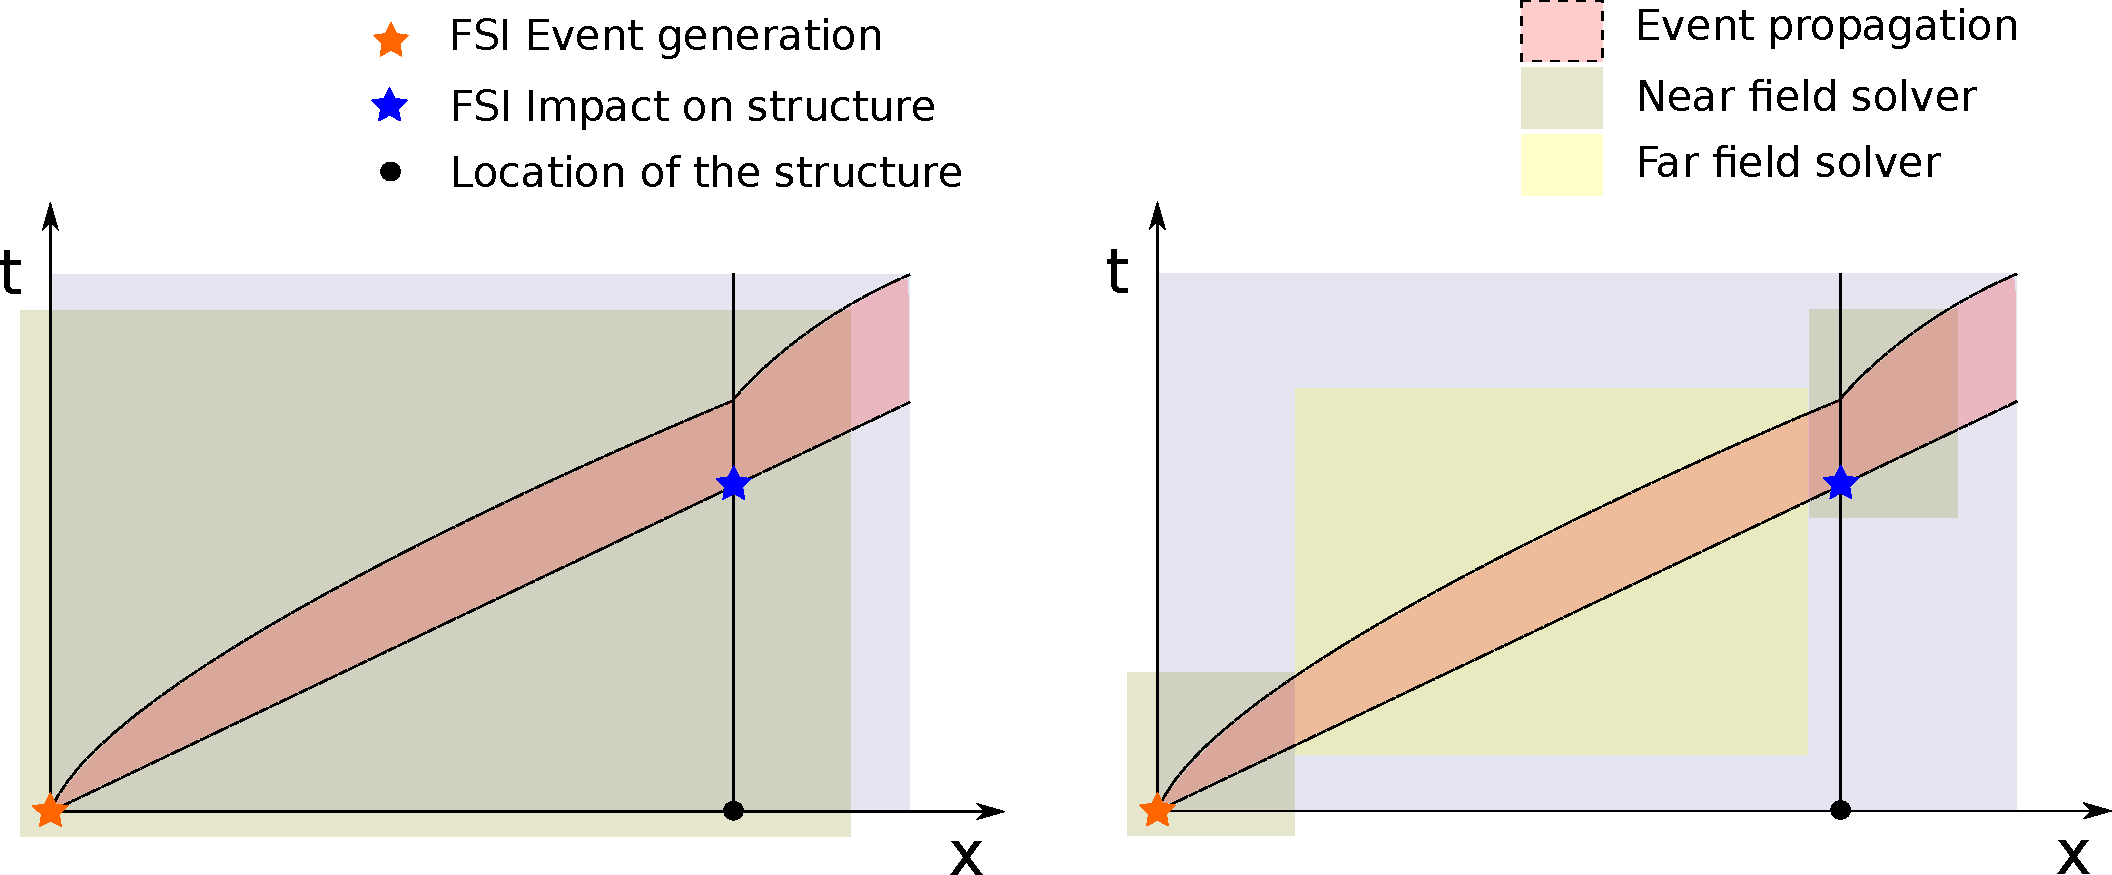
\includegraphics[width=\textwidth]{img/coupling/space_time}
    \caption{Propagation path of the event and possible computational approaches. Left: Brute force approach. Right: Staggered approach.}
    \label{space_time_staggered_approach}
\end{figure}


The main aspects that have been explored in this thesis are the numerical approximation of the FFS and the coupling strategy of the proposed FFS and an existing NFS. Special attention have been paid to the convergence and stability properties of the FFS aimed to solve the large scale.




%%%%%%%%%%%%%%%%%%%%%%%%%%%%%%%%%%%%%%%%%%%%%%%%%%%%%%%%%%%%

\section{Objectives and outline}


The work developed within the framework of this thesis can be enclosed in the global objective of investigating Finite Element formulations applied to large-scale water-related hazards. In particular, the analyzed methods have to be capable of reproducing local-scale effects around structures of interest and accurately model the large-scale propagation. This requirement lead to the analysis of the Finite Element Method for solving the Navier-Stokes equations on local scales and solving the shallow water equations on large scales.

The Navier-Stokes equations are typically solved using the finite element method, while the shallow water equations are often solved using the finite volume method.
Since we are interested in solving within the same framework the global simulation, a previous investigation on stabilized finite elements for the shallow water equations is presented.


This thesis is structured in 6 chapters, including the present introduction and a bibliographic revision. The bibliographic revision is specially extensive for the shallow water equations.
Chapter \ref{equations} presents a review of the governing equations which will be solved in the latter chapters.

Chapter \ref{eulerian_sw} is dedicated to the Finite Element Method applied to the shallow water equations. Stabilized formulations and quasi-monotonic formulations are presented.
Part of the developments of the numerical methods for the shallow water equations are moved to appendices \ref{lagrangian_sw} and \ref{mesh_refinement}, where the particle methods and mesh refinement are explored.
%This family of methods present some interesting properties, such as the natural approximation of the shoreline. The inconvenient of the Particle methods is the lack of robustness for all the possible flow regimes.

An extension of the shallow water equations to wave propagation on intermediate and deep water is presented in chapter \ref{eulerian_bsq}. These equations are known as the Boussinesq equations. The strategies developed in the previous chapter are applied to the Boussinesq equations, however, additional requirements must be fulfilled in order to ensure stability and accuracy. This chapter is of crucial importance in order to analyze impulse waves in the context of water-related hazards.

Chapter \ref{coupling} is devoted to the coupling strategies between the shallow water approximations --specially the Boussinesq equations-- and the fully resolved methods. An example of coupling for landslide long wave generation is provided.

Finally, the thesis is closed with some conclusions and possible further research lines in chapter \ref{conclusions}.


%%%%%%%%%%%%%%%%%%%%%%%%%%%%%%%%%%%%%%%%%%%%%%%%%%%%%%%%%%%%

\section{Research dissemination}


Some of the developments if this thesis have been published in the format of articles in peer reviewed journals. Since the research has advanced gradually, the articles are related to a chapter, but there are some differences, which can be big.
The chapters are more extensive than the articles and some parts of the articles are omitted to avoid repetitions.
There is also not the same sequence between the publication date and the chapter order.
On the other hand, since the notation is introduced gradually, it has been unified in the thesis and may be slightly different from the articles and this document.

\paragraph{Chapter \ref{eulerian_sw}} \fullcite{maso2022}
\paragraph{Chapter \ref{coupling}} \fullcite{maso2022b}
\paragraph{Appendix \ref{lagrangian_sw}} \fullcite{puigferrat2021}
\\

In addition, the content of the chapters has been also disseminated in the form of oral presentations in scientific conferences and congresses:

\paragraph{Chapter \ref{coupling}} WCM
\paragraph{Chapter \ref{coupling}} CMN
\paragraph{Chapter \ref{coupling}} Franci
\paragraph{Appendix \ref{lagrangian_sw}} Particles 2019

%%%%%%%%%%%%%%%%%%%%%%%%%%%%%%%%%%%%%%%%%%%%%%%%%%%%%%%%%%%%


\section{State of the art}
\label{state_art}


In this chapter a bibliographic revision of the methods employed to solve free surface flows problems is presented.
The analysis of the numerical methods for the shallow water equations is more extensive than the review for the Navier-Stokes equations, since this thesis presents some advances in the numerical simulation of the shallow water equations.



\subsection{Numerical methods for the Navier-Stokes model}

% \subsubsection{Overview}

% \subsubsection{Particle methods}



\subsection{Numerical methods for the shallow water models}


\subsubsection{Overview}

The computation of the dry-wet interface of the shallow water equations is a challenging problem. Due to the hyperbolic character of the equations the water height requires positivity ($h>0$) and oscillations can trigger global failure of the system. Löhner \cite{lohner2008} made a review of possible approximation methods to solve fluid dynamics. Being $u^h = N^i\hat{u}_i$ ($i=1,2,\dots,m$) an approximation of the solution $u$, the weighted residual is defined as

\begin{equation}
\int_{\Omega} W^ir(u^h)d\Omega = 0
\end{equation}

\begin{table}
\centering
\begin{tabular}{|l|c|c|}
\hline
 & $N^i$ & $W^i$ \\ \hline
Finite differences (FD)         & polynomial & $\delta(x_i)$ \\ \hline
Finite volumes (FV)             & polynomial & $1 \ \text{if} \ x\in\Omega_{el}$ \\ \hline
Galerkin finite elements (FEM)  & polynomial & $N^i$ \\ \hline
Discontinuous Galerkin (DG)     & polynomial & $N^i \ \text{if} \ x\in\Omega_{el}$ \\ \hline
\end{tabular}
\caption{Possible choices of trial and test functions $N^i$ and $W^i$}
\label{possible_trial_functions}
\end{table}

In table \ref{possible_trial_functions} there are a set of possible trial and test functions and the resulting approximation method. In the recent decades a new family of finite elements have been developed which are known as the discontinuous Galerkin (DG). We are interested on the implementation of \emph{continuous Galerkin finite elements} in KratosMultiphysics.


\subsubsection{Stabilized methods}



\subsubsection{Monotonicity preserving finite elements}

Following Löhner review, there are three classical approaches: stabilized finite elements \cite{lohner2008}, flux corrected transport (FCT) \cite{lohner2008ch9} and edge based finite elements \cite{lohner2008ch10}.

\paragraph*{Stabilized FEM} Streamline-diffusion methods like SUPG are stable but not
monotonicity preserving. However, Badia and Hierro presented a monotonicity preserving stabilized finite element for hyperbolic equations \cite{badia2014}.

\paragraph*{FCT} The way to circumvent the Godunov barrier theorem \cite{godunov1959} is to develop a nonlinear scheme. FCT uses a low order (LO) monotonic scheme with a lot of diffusion and a high order (HO) oscillatory scheme. The process of combining the two schemes is called limiting:

\begin{equation}
\phi^{n+1} = \phi^n + c_e\Delta \phi_H + (1-c_e)\Delta \phi_L
\end{equation}

\paragraph*{Edge based} The edge based structure is an efficient way to assemble the system matrix which resort to a
finite volume approximation of convective terms. If it is assumed that the fluxes of the variables are constant along the edges, a discontinuity will occur at the edge midpoint. Then, one can replace the Galerkin flux by a Riemann flux and obtain a total variational diminishing scheme (TVD).


% \subsubsection{Particle methods}



\subsection{Coupling strategies}





\chapter{Governing equations for free surface flows}
\label{equations}



%Before introducing the review of the numerical methods, the governing equations will be presented.
%The following sections are devoted for the numerical methods.
%The last section is about the coupling algorithms.



%\section{Free surface flows}


Water related natural hazards usually involve free surface flows.
This property allows to assume some simplifications, specially at the large scale.
For this reason, the general case describing the fluid motion is presented first, the Navier-Stokes equations.
Then, some simplifications for the free surface flows are made, yielding the shallow water equations. Different assumptions for the depth integrated models will provide different sets of equations and its range of applicability as well as physical properties will be explained.




\section{Navier-Stokes equations}
\label{equations_ns}


The motion of a fluid is described by the Navier-Stokes equations. The case of a free surface flow is described by that equations and the free surface is located where the densities or the fluid properties are discontinuous. In general, an air-water interface is assumed but some natural phenomena may include a more complex configuration, such as debris flow-air-water interfaces. All this continuous media can be considered isotermal and incompressible, and the standard formulation of the Navier-Stokes equations can be used.

The problem consists in the incompressible Navier-Stokes equations in a time interval $(0, t_f)$ and in a spatial domain $\Omega \in \mathbb{R}^{n_d}$, being $n_d$ the number of space dimensions, $3$ unless otherwise stated. Let $t$ be a certain time instant in the temporal domain $(0, t_f)$ and $\mathbf{x}$ a given point in the spatial domain $\Omega$. The balance equations for the momentum and mass are written in the following form:
\begin{subequations} \label{NS}
    \begin{align} \label{NS1}
        \pder{u_i}{t} + u_j \pder{u_i}{x_i} + \frac{1}{\rho} \pder{p}{x_i} +
            \frac{1}{\rho} \pder{}{x_i} \tau_{ij} &= f_i \\ \label{NS2}
        \pder{u_i}{x_i} &= 0
    \end{align}
\end{subequations}
With the appropriate initial and boundary conditions. Let $\Gamma$ be the boundary of the domain $\Omega$ and $\mathbf{n}$ the unit outward normal on $\Gamma$. Dirichlet and Neumann boundary conditions are considered, $\Gamma_D$ and $\Gamma_N$ respectively, such that $\Gamma_D \cup \Gamma_N = \Gamma$.
The usual summation convention is used if there is index repetition.
$\rho$ is the fluid density, $p$ is the pressure, $\mathbf{u}$ is the velocity, $\bm{\tau}$ is the viscous stresses tensor and $\mathbf{f}$ is the body forces vector.




%%%%%%%%%%%%%%%%%%%%%%%%%%%%%%%%%%%%%%%%
%%%%%%%%%%%%%%%%%%%%%%%%%%%%%%%%%%%%%%%%
%%%%%%%%%%%%%%%%%%%%%%%%%%%%%%%%%%%%%%%%




\section{Shallow water equations}
\label{equations_sw}


The flow of water in shallow layers occurs in a wide range of situations, such as coastal dynamics and hydraulics. In these free surface flows in relatively thin layers compared to the characteristic horizontal length, the horizontal velocities are of primary importance. Under that circumstances, the problem can be reasonably approximated the horizontal plane.

The shallow water equations are the result of integrating vertically the Navier-Stokes equations, assuming incompressibility, small vertical velocity and negligible vertical acceleration \cite{abbott1979,zien3}. The assumptions over the vertical velocity and its acceleration are equivalent to hydrostatic pressure, in fact, the vertical component of the momentum equation (\ref{NS1}) is reduced to
\begin{equation} \label{SW_hydrostatic_pressure}
    \frac{1}{\rho}\pder{p}{x_3} + g = 0
\end{equation}

After substitution of the hydrostatic pressure assumption \ref{SW_hydrostatic_pressure} into the mass conservation \ref{NS2}, the governing equations are integrated from the bottom $z$ to the free surface $\eta$. The problem is closed by adding two kinematic boundary conditions at the bottom and the free surface:
\begin{equation}
    u_3(\eta) = \frac{D\eta}{Dt} \ , \quad u_3(z) = \frac{Dz}{Dt}
\end{equation}


The governing equations are expressed in terms of a new set of primary variables: the water depth and the horizontal flow rate. The water depth is defined by the integration limits, $h = z + \eta$ and the averaged horizontal flow rate $\mathbf{q}$ is defined by the following integrated value,
\begin{equation} \label{SW_averaged_momentum}
    \mathbf{q} = \int_z^\eta \mathbf{u}\,dx_3
\end{equation}
To avoid introducing extra notation, in a shallow water context, $\mathbf{u}$ refers to the averaged horizontal velocities. In that case, the expression \ref{SW_averaged_momentum} can be reduced to a compact form as $\mathbf{q} = h\mathbf{u}$.


Here we find that the resulting equations are written in the same form as the Euler conservation equations. In spite the equations present some similarities to the compressible flow, the shallow water equations are describing a purely incompressible fluid: the variable water depth is playing the role of the variable pressure in compressible fluids. The equations read
%The equations governing mass and momentum conservation can be written in conservative form with water depth $h$ and specific discharge $\mathbf{q}=(h\mathbf{u})$ as follows,
\begin{equation} \label{general_sw}
\pder{\bm{\phi}}{t} + \pder{\mathbf{F}_i}{x_i} + \pder{\mathbf{G}_i}{x_i} + \mathbf{Q} = \mathbf{0} \qquad \text{for} \enspace i=1,2
\end{equation}
with

\begin{subequations}\label{variables_and_fluxes}
\allowdisplaybreaks
\begin{align}
\bm{\phi} &= \left\{
    \begin{array}{c}
        hu_1 \\
        hu_2 \\
        h
    \end{array}\right\} \\
\mathbf{F}_i &= \left\{
    \begin{array}{c}
        hu_1u_i + \delta_{1i}\frac{1}{2}g(h^2 - z^2) \\ [5pt]
        hu_2u_i + \delta_{2i}\frac{1}{2}g(h^2 - z^2) \\ [5pt]
        hu_i
    \end{array}\right\} \\
\mathbf{G}_i &= \left\{
    \begin{array}{c}
        -(h/\rho) \bar{\tau}_{1i} \\ [5pt]
        -(h/\rho) \bar{\tau}_{2i} \\ [5pt]
        0
    \end{array}\right\} \\
\mathbf{Q} &= \left\{
    \begin{array}{c}
        \displaystyle -g(h-z)\pder{z}{x_1} + \frac{h}{\rho}\pder{p_a}{x_1}
        - \frac{1}{\rho}\tau^s_{31} + \frac{1}{\rho}\tau^b_{31} \\ [10pt]
        \displaystyle -g(h-z)\pder{z}{x_2} + \frac{h}{\rho}\pder{p_a}{x_2}
        - \frac{1}{\rho}\tau^s_{32} + \frac{1}{\rho}\tau^b_{32} \\ [10pt]
        r
    \end{array}\right\}
\end{align}
\end{subequations}
where $\bm{\phi}$ is the vector of conserved variables, $\mathbf{F}_i$ is the vector of convective fluxes, $\mathbf{G}_i$ is the vector of viscous fluxes and $\mathbf{Q}$ is the vector source terms. In Figure \ref{diagram} there is a representation of the variables and the notation. The coordinates are denoted with the index notation $x_i$. Since this formulation is defined in a two dimensional space ($n_d=2$), in the following we will consider $i=1,2$.
$\delta_{ij}$ is the Kronecker delta. The topography is expressed with the variable $z$ and the free surface elevation is expressed in terms of the topography and the total depth, $\eta = z + h$. $\bar{\tau}_{ij}$ are the averaged horizontal stresses, and $\tau^b_{3i}$ and $\tau^s_{3i}$ denote the bottom and surface friction stresses respectively. Finally, $r$ is the rain source term and $p_a$ is the atmospheric pressure.


\begin{figure}
    \centering
    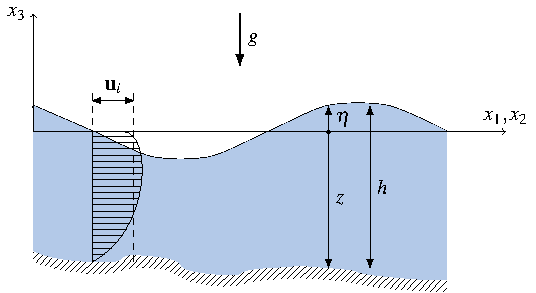
\includegraphics[width=.8\textwidth]{img/eq/diagram.pdf}
    \caption{Diagram and notation for the balance equations (\ref{general_sw}) and (\ref{variables_and_fluxes})}
    \label{diagram}
\end{figure}



Usually, the bottom friction $\tau^b_{3i}$ from (\ref{variables_and_fluxes}) is modelled with a semi-empirical formula, such as the Chezy or the Manning formula. The Manning formula generalized for two dimensions is as follows:
\begin{equation}
\frac{\tau^b_{3i}}{\rho} = -gn^2\frac{\abs{\mathbf{q}}\mathbf{q}}{h^{\sfrac{7}{3}}}
\end{equation}
where $n$ is the Manning roughness coefficient. It defines the resistance to flow by the roughness of the bottom or other macroscopic factors and it is determined empirically. In practice, the Manning coefficient varies from $0.009$ for a very smooth bed (concrete) to $0.05$ for a rough bed (rocks) \cite{chow1988}.


The averaged horizontal stresses are calculated from the combination of the molecular stresses and the Reynolds stresses as follows
\begin{equation} \label{stresses}
\frac{\bar{\tau}_{ij}}{\rho} = (\nu + \nu_t)\left(
    \pder{u_i}{x_j} + \pder{u_j}{x_i} -\frac{2}{3}\delta_{ij}\pder{u_k}{x_k} \right)
\end{equation}
where $\nu$ is the kinematic viscosity and $\nu_t$ is the turbulent kinematic viscosity. When any model of turbulence is considered, the turbulent stresses can be considered as included in the bottom friction with the Manning formula \cite{blade2005}. In this work, the turbulent stresses will be neglected.



Returning again to the equations structure, the Euler conservation laws define two eigenvalues fo the one-dimensional case: $\lambda = u \pm c$. Where $u$ is the modulus of the velocity and $c=\sqrt{gh}$ is the phase speed or wave speed.
In the case of positive eigenvalues, the flux is supercritical, this means that the information travels in one direction, the velocity is higher than the phase speed. When the eigenvalues are of different sign, the flow is subcritical. If one of the eigenvalues is zero, the flow becomes critical and is unstable, so it will derive to a stable solution, sub or supercritical.

For the two dimensional case, does not exist a unique decomposition and this is known as amplitude dispersion. This means there is not an unique direction of propagation. The projection to the velocity direction -the main direction- will provide the eigenvalues $\lambda_1 = u - c$, $\lambda_2 = u$ and $\lambda_3 = u + c$.



%%%%%%%%%%%%%%%%%%%%%%%%%%%%%%%%%%%%%%%%
%%%%%%%%%%%%%%%%%%%%%%%%%%%%%%%%%%%%%%%%



\subsection{Boundary conditions}
\label{equations_sw_bc}


The problem is closed with appropriate boundary conditions: an initial condition
\begin{equation}
\bm{\phi}(t=t_0) = \bm{\phi}_0
\end{equation}
where $\bm{\phi}_0$ are the initial water height and specific discharge. And boundary conditions at $\Gamma$, being $\Gamma$ the boundary of the domain $\Omega$. The boundary $\Gamma$ is split into three subdomains, $\Gamma_I$, $\Gamma_O$ and $\Gamma_S$: inflow, outflow and solid.
\paragraph{Inflow boundary} the flow rate is known
\begin{equation*}
    \mathbf{q} = \mathbf{q}_{in} \quad \text{in} \quad \Gamma_{in}
\end{equation*}
If the inflow is supercritical, the water depth is also specified
\begin{equation*}
    \left.\begin{matrix}
    \mathbf{q} = \mathbf{q}_{in} \\
    h = h_{in}
    \end{matrix}\right\}
    \quad \text{in} \quad \Gamma_{in}
\end{equation*}


\paragraph{Outflow boundary} The water depth is known
\begin{equation*}
    h = h_{out} \quad \text{in} \quad \Gamma_{out}
\end{equation*}
if the outflow is supercritical, no conditions have to be imposed.


\paragraph{Solid boundary} slip or no slip condition can be imposed
\begin{equation*}
    \mathbf{q} \cdot \mathbf{n} = 0 \quad \text{or} \quad \mathbf{q} = \mathbf{0} \quad \text{in} \quad \Gamma_{solid}
\end{equation*}



%%%%%%%%%%%%%%%%%%%%%%%%%%%%%%%%%%%%%%%%
%%%%%%%%%%%%%%%%%%%%%%%%%%%%%%%%%%%%%%%%



\subsection{Linearization}

Usually, in the numerical study of the conservation equations, them are expressed in a quasi-linear form. The balance equation (\ref{general_sw}) can be linearized as follows


\begin{equation} \label{general_sw_lin}
\pder{\bm{\phi}}{t} + \mathbf{A}_i\pder{\bm{\phi}}{x_i}
 - \pder{}{x_{i}}\left(\mathbf{K}_{ij}\pder{\bm{\phi}}{x_j}\right) + \mathbf{S}\bm{\phi} + \mathbf{b}_i\pder{z}{x_i} = 0
\end{equation}
where the matrices $\mathbf{A}_i$ and $\mathbf{K}_{ij}$ are the linearization matrices of the convective fluxes and the diffusive fluxes respectively. The convective matrices $\mathbf{A}_i$ are obtained after applying the chain rule to the vector of fluxes $\mathbf{F}_i$,
\begin{subequations}
\begin{align}
\pder{\mathbf{F}_i}{x_i} &= \pder{\mathbf{F}_i}{\bm{\phi}}\pder{\bm{\phi}}{x_i} \\
\mathbf{A}_i &= \pder{\mathbf{F}_i}{\bm{\phi}}
\end{align}
\begin{equation}
    \mathbf{A}_1 = \left[\begin{matrix}
        2u_1 & 0   & -u_1^2 + gh \\
        u_2  & u_1 & -u_1 u_2 \\
        1    & 0   & 0
    \end{matrix} \right]
    \quad , \quad
    \mathbf{A}_2 = \left[\begin{matrix}
        u_2 & u_1  & -u_1 u_2 \\
        0   & 2u_2 & -u_2^2 + gh \\
        0   & 1    & 0
    \end{matrix} \right]
\end{equation}
\end{subequations}
As seen before, the equation (\ref{general_sw}) is characterized by three eigenvalues. Those eigenvalues are defined by the matrices $\mathbf{A}_i$. 
For the one dimensional case, there is a unique definition of the eigenvalues, $\lambda_{1,2}=u\pm c$.
In two dimensions, given the unit vector $\mathbf{e}$, the eigenvalues of the matrix $e_i \mathbf{A}_i$ are $\lambda_{1,3} = \mathbf{e}\cdot\mathbf{u} \pm c$ and $\lambda_2 = \mathbf{e}\cdot\mathbf{u}$.
The eigenvalues are real and always different ($\lambda_1<\lambda_2<\lambda_3$), this property is called strictly hyperbolicity \cite{raviart1996}. The eigenvalues are velocities, namely the ones of surface waves on the fluid. Note that in the dry zones, where ${h=0}$, the eigenvalues coincide and the system is no longer hyperbolic. This introduces difficulties at theoretical and numerical level.


The vectors $\mathbf{b}_i$ are the result of the linearization of the topography using the same procedure taken for $\mathbf{A}_i$. They are obtained by the linearization of the fluxes $\mathbf{F}_i$ respect to the topography coordinate $z$. Rearranging terms with the independent vector $\mathbf{Q}$ yields
\begin{equation}
    \mathbf{b}_i = \left[\begin{matrix}
        \delta_{i1} c^2 \\
        \delta_{i2} c^2 \\
        0
    \end{matrix}\right]
\end{equation}


Analogously, the viscous fluxes $\mathbf{G}_i$ are rewritten in a more convenient manner as ${\mathbf{G}_i = \mathbf{K}_{ij} \partial\bm{\phi}/\partial x_j}$. The fourth order tensor $\mathbf{K}_{ij}$ is obtained making use of equation (\ref{stresses}). It is an auxiliary variable to write the linearized tensor in Voigt's notation. This tensor will be defined latter, in the numerical model section.




The bottom friction term acting on the source term vector is linearized using a reaction matrix $\mathbf{S}$
\begin{equation}
\mathbf{S} = \left[\begin{matrix}
    \frac{gn^2\abs{\mathbf{u}}}{h^{4/3}} & 0 & 0 \\
    0 & \frac{gn^2\abs{\mathbf{u}}}{h^{4/3}} & 0 \\
    0 & 0 & 0
\end{matrix}\right]
\end{equation}
In the following sections, the rain, the atmospheric pressure and the wind friction will be neglected.




%%%%%%%%%%%%%%%%%%%%%%%%%%%%%%%%%%%%%%%%
%%%%%%%%%%%%%%%%%%%%%%%%%%%%%%%%%%%%%%%%
%%%%%%%%%%%%%%%%%%%%%%%%%%%%%%%%%%%%%%%%




\section{Shallow water equations with primitive variables}


The presented, conservative, form of the shallow water equations --Saint-Venant equations-- is generally applicable. However, many variations are present in the literature.
The most common simplification is to express those equations in terms of the reduced or primitive variables --velocity instead of flow rate--.
Another alternative is to use relative variables, taking the free surface instead of the total water depth.

The primitive variables simplification reduces the non-linearity of the equations, while its range of applicability is reduced. Particularly, the momentum would not be conserved in a change of regime, an hydraulic jump. This fact is related to the evaluation of the convective fluxes, which depend on the flow rate gradient.
While the evaluation of the flow rate gradient using conservatives variables does not present any problem, this operation will be ill-conditioned when primitive variables are used.
In other words, in a change of regime there is a discontinuity in both velocity and water depth, and the computation of the flow rate gradient involves the division of two gradient tending to $\pm\infty $.

In spite of this accuracy limitation near shocks, the non linearity reduction makes the primitive variables interesting from the numerical point of view, since less iteration will be needed to achieve convergence.
Furthermore, good results are obtained for flows at low Froude numbers, such as estuaries, tidal currents or waves propagation.



%%%%%%%%%%%%%%%%%%%%%%%%%%%%%%%%%%%%%%%%
%%%%%%%%%%%%%%%%%%%%%%%%%%%%%%%%%%%%%%%%



\subsection{Equations}


The non linearity of the shallow water equations can be reduced if they are expressed in terms of the velocity. The primitive SWE can be obtained by replacing the mass balance equation into the momentum balance and expanding the derivatives:
\begin{subequations} \label{sw_primitive_balance}
\begin{equation}
    \pder{\bm{\psi}}{t} + \pder{\mathbf{F}_i}{x_i} + \mathbf{Q} = \mathbf{0}
\end{equation}
\begin{align} \label{sw_primitive_balance:vectors}
    \bm{\psi} &= \left\{\begin{array}{c}
        \mathbf{u} \\ h
    \end{array}\right\} \\
    \mathbf{F}_i &= \left\{\begin{array}{c}
        u_1 u_i + \delta_{1i}g(h-z_b) \\
        u_2 u_i + \delta_{2i}g(h-x_b) \\
        u_i h
    \end{array}\right\} \\
    \mathbf{Q} &= \left\{\begin{array}{c}
        gS_1 \\ gS_2 \\ 0
    \end{array}\right\}
\end{align}
\end{subequations}

The same linearization procedure can be applied if the variables $\psi$ are smooth enough. The following quasi-linear formulation will be obtained after applying the chain rule,
\begin{equation}
    \pder{\bm\psi}{t} + \mathbf{A}_i\pder{\bm\psi}{x_i} + \mathbf{S}\bm{\psi} + \mathbf{b}_i\pder{z}{x_i} = 0
\end{equation}
where the tangent matrices $\mathbf{A}_i$ have been defined according to the differentiation of the convective fluxes with respect to the unknowns, $\partial\mathbf{F}_i/\partial\bm{\psi}$. 
Analogously, the same procedure is applied to the topography terms and to the bottom friction. The expression of the tangent matrices is
\begin{equation}
    \mathbf{A}_1 = \left[\begin{array}{ccc}
        u_1 &  0  &  g  \\
         0  & u_2 &  0  \\
         h  &  0  & u_1
    \end{array}\right] \quad , \quad
    \mathbf{A}_2 = \left[\begin{array}{ccc}
        u_1 &  0  &  0  \\
         0  & u_2 &  g  \\
         0  &  h  & u_2
    \end{array}\right]
\end{equation}




%%%%%%%%%%%%%%%%%%%%%%%%%%%%%%%%%%%%%%%%
%%%%%%%%%%%%%%%%%%%%%%%%%%%%%%%%%%%%%%%%
%%%%%%%%%%%%%%%%%%%%%%%%%%%%%%%%%%%%%%%%




\section{Boussinesq modified equations}
\label{equations_bsq}


The presented SWE are suited to solve convective flows as well as free surface waves. Both phenomena are present in the hyperbolic equations. As the water depth increases, the oscillatory phenomenon or amplitude dispersion increases its relative importance.
However, a new mechanism not included in the SWE is present in a wave propagation problem, the frequency dispersion \cite{ursell1953}. A need to quantify the relative importance of the new mechanism arises.

According to the classification of Peregrine \cite{peregrine1967}, the dimensionless numbers of non-linearity and dispersion relate the wave amplitude $\eta$, the water depth $H$ and the characteristic wavelength $\lambda$:

\begin{equation}
    \epsilon = \frac{\eta}{H} \ ,\quad \mu = \frac{H}{\lambda}
    \label{nonlin_disp_ratios}
\end{equation}

Both parameters allow to relate the concepts of amplitude and frequency dispersion. These concepts define how the wave propagates. Is well known that a wave propagates at speed $c=\sqrt{gH}$, but due to the convective term, this speed also depends on the wave amplitude, then introducing a non-linearity. Thus, considering the non-linearity, the wave speed increases as $c=\sqrt{g(H+\eta)}$. This phenomenon is known as amplitude dispersion and a first consequence is that every wave will end breaking, since the wave crest propagates faster than the wave bosom. The importance of the amplitude dispersion is related to the non-linearity ratio $\epsilon$.


\begin{figure} [ht]
    \centering
    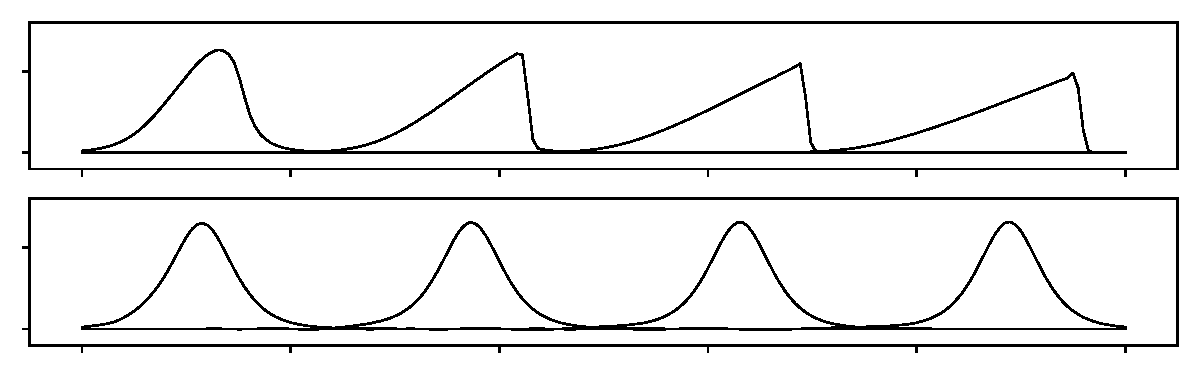
\includegraphics[width=.95\textwidth]{img/eq/boussinesq_dispersion.pdf}
    \caption{Boussinesq equations. Snapshots of a wave propagation. Top: Amplitude dispersion. Bottom: Frequency dispersion}
    \label{boussinesq_dispersion}
\end{figure}


In practice, this phenomenon does not happen. From linear wave theory we know that the celerity depends not only on the water depth, but also on the wavenumber $k=2\pi/\lambda$. This is known as frequency dispersion and this mechanism is missing on the Saint-Venant equations. The introduction of some extra terms leads to the Boussinesq equations, which model the frequency dispersion. Once the frequency dispersion is included, classical soliton waves can be obtained. In a soliton wave, breaking never occurs during the propagation, since the non linear terms are in equilibrium with dispersive terms.



%%%%%%%%%%%%%%%%%%%%%%%%%%%%%%%%%%%%
%%%%%%%%%%%%%%%%%%%%%%%%%%%%%%%%%%%%



\subsection{Derivation of the modified Boussinesq equations}

There are different ways to derive the Boussinesq equations with slightly different results. Nwogu presented a general framework in \cite{nwogu1993}. A three dimensional wave field with free surface elevation $\eta(x_1, x_2, t)$ and water depth at rest $H(x_1, x_2)$ is considered. The fluid is governed by the Navier-Stokes equations but the shallow water assumptions are modified. The fluid is assumed to be incompressible and the flow is assumed to be irrotational. As in the shallow water equations, the vertical velocity is considered to be small, but the vertical acceleration is not negligible. The nonlinearity and dispersion ratios (\ref{nonlin_disp_ratios}) are assumed to be small. The last difference between the shallow water equations and the Boussinesq consist in considering the horizontal velocity at a specified water depth instead of the mean value.

\begin{figure}
    \centering
    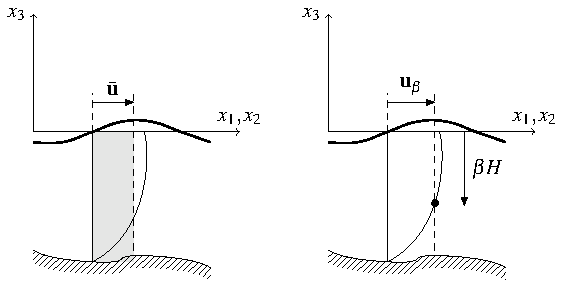
\includegraphics[width=.9\textwidth]{img/eq/velocity_beta.pdf}
    \caption{The modified Boussinesq equations consider the velocity at an arbitrary depth $\beta H$ instead of the mean velocity}
\end{figure}

Finally, the fluid at the free surface has to satisfy a dynamic and kinematic boundary conditions. At the bottom, the fluid has to satisfy a kinematic boundary condition.

\begin{equation}\label{dyn_kyn_bc}
\begin{aligned}
p &= 0 \ , \quad &&\text{at } x_3=\eta \\
u_3 &= \pder{\eta}{t} + u_1 \pder{\eta}{x_1}  + u_2 \pder{\eta}{x_2} \ , \quad &&\text{at } x_3=\eta \\
u_3 &= -u_1 \pder{H}{x_1} -u_2 \pder{H}{x_2} \ , \quad &&\text{at } x_3=-H
\end{aligned}
\end{equation}

Then, the continuity and momentum equations are integrated from the bottom to the free surface and applying the boundary conditions (\ref{dyn_kyn_bc}). Since the average horizontal velocity has been substituted by the velocity at a certain depth, the vertical profile of the velocities must be known. The key of the Boussinesq equations consist in finding an assumption which preserves the the effect of the frequency dispersion. The horizontal velocities $\mathbb{u}=(u_1, u_2)$ are expanded in Taylor series from the seabed ($x_3=-H$),
\begin{multline} \label{seabed_taylor_expansion}
    \mathbf{u}(x_1,x_2,x_3,t) = \mathbf{u}(x_1,x_2,-H,t) + (z+H)\mathbf{u}_3(x_1,x_2,-H,t) \\ + \sfrac{1}{2}(z+H)^2\mathbf{u}_{3,3}(x_1,x_2,-H,t) + \dots
\end{multline}
where the $3$ subscript denotes differentiation with respect to $x_3$.
Finally, the equations are evaluated at an arbitrary depth $x_3=\beta H$ and the set of Boussinesq-type equations are:

\begin{subequations} \label{bsq_eq}
\begin{equation} \label{bsq_eq_mom}
    \pder{\mathbf{u}_\beta}{t} + \nabla \eta + (\mathbf{u}_\beta \cdot \nabla) \mathbf{u}_\beta + \mathbf{J}_u = \mathbf{0}
\end{equation}
\begin{equation} \label{bsq_eq_mass}
    \pder{\eta}{t} + \nabla \cdot \left((H+\eta)\mathbf{u}_\beta\right) + \nabla \cdot \mathbf{J}_\eta = 0
\end{equation}
\end{subequations}
where the auxiliary fields $\mathbf{J}_\eta$ and $\mathbf{J}_u$ introduce the dispersive mechanism and are defined according to the following expressions
\begin{subequations} \label{bsq_eq_auxiliary_J}
\begin{equation}
    {J}_\eta =
        C_1 H^3 \nabla \nabla \cdot \mathbf{u}_\beta +
        C_3 H^2 \nabla \nabla \cdot (H \mathbf{u}_\beta) 
\end{equation}
\begin{equation}
    {J}_u =
        C_2 H^2 \nabla \nabla \cdot \pder{\mathbf{u}_\beta}{t} +
        C_4 H   \nabla \nabla \cdot \pder{(H \mathbf{u}_\beta)}{t} 
\end{equation}
\end{subequations}
and the $C_i$ constants depend on the choice of $\beta$
\begin{equation} \label{bsq_eq_C_constants}
    C_1=\frac{1}{2}\left(\beta^2-\frac{1}{3}\right)\ ,
    C_2=\frac{\beta^2}{2}\ ,
    C_3=\beta + \frac{1}{2}\ ,
    C_4=\beta
\end{equation}



%%%%%%%%%%%%%%%%%%%%%%%%%%%%%%%%%%%%%%%%
%%%%%%%%%%%%%%%%%%%%%%%%%%%%%%%%%%%%%%%%



\subsection{Dispersion properties and range of applicability}

This equations present as a free parameter $\beta$ the relative elevation at which the velocity is evaluated. Its value goes from $-1$ at the seabed, to $0$ at the free surface. Since the equations are an approximation of the fully dispersive and nonlinear problem, the parameter $\beta$ is chosen to minimize the errors introduced by the approximation.
In fact, the original Boussinesq equations does no present any dispersive term in the mass balance equation (\ref{bsq_eq_mass}) and correspond to a specific choice of $\beta$.

The parameter $\beta$ is fixed to $-0.531$ in \cite{nwogu1993}. This value has been obtained reducing the equations (\ref{bsq_eq}) to one dimension and flat bottom. Then, a trial function of small amplitude periodic wave of the type
\begin{equation*}
    \eta = a_0 \exp(i(kx-\omega t)) \ , \quad u_\beta = u_0 \exp(i(kx-\omega t))
\end{equation*}
is substituted into (\ref{bsq_eq_mass}) and (\ref{bsq_eq_mom}). After some algebraic manipulation the following expression for the phase speed is obtained:
\begin{equation}
c^2 = \frac{\omega^2}{k^2} = gh
    \left(\frac{
        1-\left(\frac{1}{2}\beta^2 + \beta + \frac{1}{3}\right)(kh)^2
    }{
        1-\left(\frac{1}{2}\beta^2 + \beta\right)(kh)^2
    }\right)
\end{equation}
The relation between the frequency and the wavelength is also known as \emph{dispersion relation}.
By the other hand, the dispersion relation given by the Linear wave theory or Airy theory is given by
\begin{equation}
c^2 = gh \frac{\tanh kh}{kh}
\end{equation}

Finally, the value of $\beta$ has been chosen to minimize the error at the range of applicability. Some other classical values of beta were obtained in \cite{madsen1991,murray1989}. Figure \ref{phase_speed_beta} shows the sensitivity of the phase speed depending on the parameter $\beta$. The shallow water equations, which drop the dispersive terms of equations (\ref{bsq_eq}) are only valid for the shallow water regime ($kh<0.3$). Fixing the free parameter $\beta=-0.531$ extend the range of applicability of the Boussinesq equations to intermediate depths ($kh<3$).

\begin{figure}
    \centering
    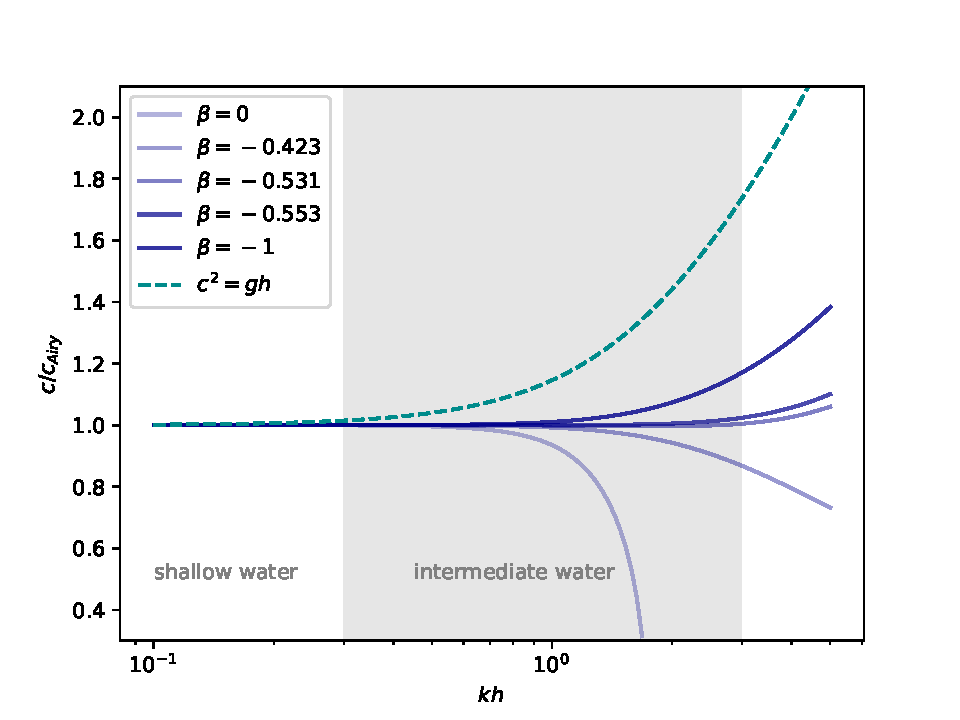
\includegraphics[width=.8\textwidth]{img/eq/dispersion_beta.pdf}
    \caption{Comparison of normalized phase speeds of the Boussinesq modified equations for different values of $\beta$}
    \label{phase_speed_beta}
\end{figure}

According to \cite{ursell1953} the nonlinearity and dispersion parameters $\epsilon$ and $\mu$ can be used for an alternative classification:

\begin{description}
    \item[$\epsilon \ll \mu$]  This configuration correspond to the case where frequency dispersion dominates the problem and linear or Airy theory must be used.
    \item[$\epsilon \sim \mu$] In this case frequency and amplitude dispersion are of the same magnitude and the Boussinesq approximation can be used.
    \item[$\epsilon \gg \mu$] In this situation the amplitude dispersion dominates the problem and the wave will eventually break. This can be simulated using the Saint-Venant or shallow water equations. Since the vertical velocity is assumed negligible, the pressure distribution is assumed to be constant.
\end{description}



%%%%%%%%%%%%%%%%%%%%%%%%%%%%%%%%%%%%%%%%%%%
%%%%%%%%%%%%%%%%%%%%%%%%%%%%%%%%%%%%%%%%%%%



\subsection{Boundary conditions}
\label{equations_bsq_bc}


The boundary conditions presented in section \ref{equations_sw_bc} are applicable to the Boussinesq equations.
However, since the oscillatory behavior is usually prevalent over the convective phenomenon, the boundary conditions are slightly different, both from the physical and the numerical point of view.
The three types of boundary conditions considered for the Boussinesq problems, inflow $\Gamma_I$, reflecting $\Gamma_R$ and absorbing $\Gamma_A$ boundaries have a direct equivalence respectively with the inflow $\Gamma_I$, solid $\Gamma_S$ and outflow $\Gamma_O$ boundaries stated in section \ref{equations_sw_bc}. Those subdomains are such that $\Gamma_I \cup \Gamma_R \cup \Gamma_A = \partial \Omega$, being $\partial\Omega$ the boundary of the domain.

\paragraph{Inflow boundary} Both free surface and velocity are known at $\Gamma_I$. Typically it is used to impose a wave generator. Since the wave amplitude is known, the horizontal velocity can be obtained using linear wave theory.

\paragraph{Reflecting boundary} No fluid should pass through an impermeable wall. This implies imposing the normal component of the velocity to be zero.
\begin{equation*}
    \bar{\mathbf{u}} \cdot \mathbf{n} = 0 \quad \text{on} \ \Gamma_R
\end{equation*}
Following Woo and Liu \cite{woo2004a}, the above relation must be rewritten in terms of $\mathbf{u}_\beta$ and the velocities are related as
\begin{equation*}
    \bar{\mathbf{u}} = \mathbf{u}_\beta + H^{-1} \mathbf{J}_\eta
\end{equation*}
Hence, the complete formulation of a reflective boundary is
\begin{equation}
    \bar{\mathbf{u}}_\beta \cdot \mathbf{n} = 0 \quad
    \mathbf{J}_\eta \cdot \mathbf{n} = 0 \quad
    \text{on} \ \Gamma_R
\end{equation}

\paragraph{Absorbing boundary} An outgoing wave should not return to the computational domain through $\Gamma_A$. A practical implementation of the absorbing boundaries are the sponge layers \cite{israeli1981, wei1995} and will be explained in section \ref{eulerian_bsq_absorbing}







\chapter{Finite Element Methods for the shallow water equations}
\label{eulerian_sw}


Due to the complexity of the geometry and the source terms, it is not possible to find an analytical solution for the SW equations. This explains the need to design strategies to find numerical solutions. In this chapter some numerical strategies with the FEM in an eulerian framework are explored.
The Eulerian frameworks are robust and very efficient for continuous problems. However, discontinuities and front tracking may require especial attention. Since flooding or moving shoreline are part of the physical phenomena of interest, the identification of the dry domain is a challenging problem for the Eulerian FEM.
Moreover, monotonic properties are especially interesting when partially wet domains are considered because the water depth is a positive magnitude but, in general, numerical methods do not verify this property.

The SW equations have traditionally been modelled using finite volumes (FV) because of its advantages of stability and monotonicity. Given its geometric flexibility and its natural way to introduce high order schemes, the FEM has been applied too \cite{zien3,navon1979,navon1988}.
Halfway between FV and FEM, there is the discontinuous Galerkin (DG) technique \cite{ambati2007,khan2014,lee2019}. DG method has the advantages of the geometrical flexibility of the FEM and the stability of FV, but the introduction of high order DG schemes is not straightforward.
Since the FEM can exhibit spurious oscillations, different strategies such as stabilization, monotonic schemes or different order of polynomial interpolation can be explored \cite{hood1974,zien3,ortiz2012}.




%This research is focused in classical stabilized finite elements with an equal order interpolation for all the variables. We will explore the capabilities of the finite increment calculus (FIC) technique to develop stable formulations for the SW equations.

In this chapter, the general procedure for FEM is presented. Then, some stabilization techniques are explored: the \emph{Finite Increment Calculus} (FIC) stabilization, the \emph{Flux Correction} (FC) technique and the \emph{Gradient jump viscosity} (GJV) methods. Several examples are provided to show the capabilities and limitations of each method.




\section{Galerkin weak formulation}



We consider a balance equation in the space domain $\Omega$ and the time interval $[0,T]$. Let $\bm{\phi}$ and $W$ be vector functions of the domain $\Omega \times [0,T]$ and $\mathbf{r}$ the residual of the balance equations expressed in terms of the unknown $\bm{\phi}$.
The space of functions that are square-integrable in $\Omega$ is denoted as $L^2(\Omega)$. And the space of functions whose derivatives up to order $m\geq0$ belong to $L^2(\Omega)$ is denoted by $H^m(\Omega)$. The space $H_0^1(\Omega)$ consists on a subspace of $H^1(\Omega)$ vanishing on $\partial \Omega$.

Using this notation, the space of functions for the continuous problem are $V \defeq H^1(\Omega)$ and for the test functions $V_0 \defeq H_0^1(\Omega)$.
The variational form of the balance equations can be expressed as find $\bm{\phi} \in V$ such that $\forall W \in V_0$
\begin{equation} \label{variational_form}
    \int_\Omega W \cdot \mathbf{r}(\bm{\phi}) \ d\Omega = 0
\end{equation}



The standard Galerkin approximation \ref{variational_form} is straightforward. Let $\mathcal{P}_h$ be a partition of the domain $\Omega$. The diameter of an element domain $e\in\mathcal{P}_h$ is denoted by $l_e$. From the polynomial spaces defined by the finite elements, we can construct the subspaces $V_h\in V$ and $V_{h,0}\in V_0$. The Galerkin approximation of the balance equations can be expressed as find $\bm{\phi}_h \in V_h$ such that $\forall W_h \in V_{h,0}$
\begin{equation} \label{discrete_variational}
    \int_\Omega W_h \cdot \mathbf{r}(\bm{\phi}_h) \ d\Omega = 0
\end{equation}

Unfortunately, this problem is not straightforward to solve using finite elements, as its discrete version is not numerically stable. In fact, to ensure that the problem of finding $\bm{\phi}_h$ has a stable solution, the space must verify the inf-sub condition \cite{codina2011}.



% We consider a balance equation in the space domain $\Omega$ and the time interval $[0,T]$. Let $\bm{\phi}$ and $\bm{\psi}$ be vector functions of the domain $\Omega \times [0,T]$ and $\mathbf{r}$ the residual of the balance equations expressed in terms of the unknown $\bm{\phi}$.
% The space of functions that are square-integrable in $\Omega$ is denoted as $L^2(\Omega)$. And the space of functions whose derivatives up to order $m\geq0$ belong to $L^2(\Omega)$ is denoted by $H^m(\omega)$. The space $H_0^1(\Omega)$ consists on a subspace of $H^1(\Omega)$ vanishing on $\partial \Omega$.

% Using this notation, the space of functions for the continuous problem are $V \defeq H^1(\Omega)$ and for the test functions $V_0 \defeq H_0^1(\Omega)$.
% The variational form of the balance equations can be expressed as find $\bm{\phi} \in V$ such that $\forall \bm{\psi} \in V_0$
% \begin{equation} \label{variational_form}
%     \int_\Omega \bm{\psi} \cdot \mathbf{r}(\bm{\phi}) \ d\Omega = 0
% \end{equation}



% The standard Galerkin approximation \ref{variational_form} is straightforward. Let $\mathcal{P}_h$ be a partition of the domain $\Omega$. The diameter of an element domain $e\in\mathcal{P}_h$ is denoted by $l_e$. From the polynomial spaces defined by the finite elements, we can construct the subspaces $V_h\in V$ and $V_{h,0}\in V_0$. The Galerkin approximation of the balance equations can be expressed as find $\bm{\phi}_h \in V_h$ such that $\forall \bm{\psi} \in V_{h,0}$
% \begin{equation} \label{discrete_variational}
%     \int_\Omega \bm{\psi} \cdot \mathbf{r}(\bm{\phi}) \ d\Omega = 0
% \end{equation}

% Unfortunately, this problem is not straightforward to solve using finite elements, as its discrete version is not numerically stable. In fact, to ensure that the problem of finding $\bm{\phi}$ has a stable solution, the space must verify the inf-sub condition \cite{codina2011}.



\section{Stabilized formulations for the shallow water equations}
\label{sec:fic_fem_stabilization}


Several families of stabilization methods can be found in the literature, usually applied to the convection-diffusion equations and the Navier-Stokes equations. The most relevant are SUPG \cite{brooks1982},
ASGS\cite{codina1998}, GLS \cite{hughes1989} and FIC\cite{onate1996,onate1998}.
Due to the hyperbolic character of the SW equations, a particular stabilization method for compressible flow or the Euler equations need to be developed.
The FIC approach is based on the incremental solution of a modified system of non-local governing equations accounting for higher order terms obtained by applying the balance laws in domains of finite size.
The FIC-based stabilization has been applied in conjunction with the FEM to convection-diffusion and incompressible flows, and solid mechanics \cite{onate1998,onate2001,onate2016}.
In those cases, where the convective term has an important role, a first order FIC term is enough to provide stability to the system.
However, the SW equations are governed by the convective term and the wave equation in a mixed formulation \cite{codina2008}. In consequence, the common derivation of the FIC-based stabilization is not enough to provide stability in all the range of applicability of the SW equations. 
A generalization of this method is proposed in order to provide a global stability for the SW equations.

Once global stability is achieved, local instabilities may appear near discontinuities, which are inherent to the supercritical flows.
A local shock capturing technique was initially proposed by Hughes \cite{hughes1986iv} and a review of shock capturing techniques can be found in Codina \cite{codina2011}.
Other possibilities of the FIC-based formulations are explored to provide a shock capturing stabilization \cite{cotela2016}.

Additionally, the dry domain requires an accurate modeling because the hyperbolic equations require positive water depth in all the domain.
Several authors have proposed different methods to solve the shallow water equations with moving shoreline. Leclerc et al. \cite{leclerc1990} proposed an Eulerian method. Later, Heniche et al. \cite{heniche2000} modified the method allowing the free surface to plunge under the topography.
Other authors developed a rough-porous layer \cite{candy2017,barros2011} or a modified depth integration \cite{defina2000}. These approaches introduce new physical parameters in the balance equations.
An Eulerian approach based on the work of \cite{leclerc1990} and \cite{heniche2000} is presented in this thesis.




\subsection{FIC stabilization}
\label{sec:stabilization}

Let us start considering the quasi-linear balance equations written in residual form as a vector

\begin{equation} \label{residual}
\mathbf{r} \defeq 
  \pder{\bm{\phi}}{t} + \mathbf{A}_i\pder{\bm{\phi}}{x_i}
  -\pder{}{x_i}\left(\mathbf{K}_{ij}\pder{\bm{\phi}}{x_j}\right) + \mathbf{S}\bm{\phi} + \mathbf{b}_i\pder{z}{x_i} \qquad i,k\in\{1,n_d\}
\end{equation}
where $n_d=2$ is the number of dimensions. The size of the vector $\mathbf{r}$ is equal to the number of balance equations, $n_b=3$.

In the one dimensional case ($n_d=1$) and scalar balance ($n_b=1$), the FIC-based stabilization is based on a modified non local version of the governing equations \cite{onate1998}, where the fluxes are expanded using a Taylor approximation. The modified residual reads
\begin{equation}
r - \frac{1}{2}l^e\pder{r}{x} = 0
\end{equation}

The stabilization parameter $l^e$ is usually taken the element length. However, in 2D and 3D, or when the number of balance equations $n_b$ is different than $n_d$, the choice of the $l^e$ parameter is non trivial.
Several approaches can be found in the literature. In \cite{onate1998} $l^e$ is chosen as a vector, but in later publications such as \cite{onate2001} a generalized formulation for different values of $n_d$ and $n_b$ was presented.
For the stabilization of the Navier-Stokes equations different projections of the element size over the velocity and over the velocity gradient have been proposed \cite{cotela2016}. Here we will use index notation for the residual vector $\mathbf{r}$ in order to distinguish the indices that goes to $n_d$ or to $n_b$. To sum up, the different forms of the FIC stabilization procedure can be written as

\begin{subequations}
\begin{align}
r_{k} - \frac{1}{2}l^e_i\pder{r_k}{x_i} &= 0
    \qquad i\in\{1,n_d\} \ ,\ k\in\{1,n_b\}\\[5pt]
r_{k} - \frac{1}{2}l^e_u\frac{u_i}{\norm{\mathbf{u}}}\pder{r_k}{x_i} &= 0
    \qquad i,k\in\{1,n_d\}\\[5pt]
r_{k} - \frac{1}{2}l^e_{g_i}\frac{\sfrac{\partial\mathbf{u}}{\partial x_i}}{\norm{\nabla u_i}}\pder{r_k}{x_i} &= 0
    \qquad i,k\in\{1,n_d\}
\end{align}
\end{subequations}

We propose a stabilization term which is oriented along the characteristics of the hyperbolic equations, as

\begin{equation} \label{fic_sw}
r_{k} - \frac{1}{2}l^e\frac{\mathbf{A}_i}{\lambda}\pder{r_k}{x_i} = 0
    \qquad i\in\{1,n_d\} \ ,\ k\in\{1,n_b\}
\end{equation}
For consistency the linearization matrix $\mathbf{A}_i$ is normalized with the maximum eigenvalue $\lambda=\abs{\mathbf{u}} + c$. This stabilization is analogue to the virtual multi-scale stabilization proposed in \cite{codina2008b}. The linearization matrix $\mathbf{A}_i$ provides a weighting procedure between the stabilization of the convective and the mixed wave equation terms. In practice the element size is multiplied by an algorithmic constant in order to control the amount of diffusion added by the stabilization and it will be studied in the examples of Section \ref{sec:examples}. Recovering the vector notation for the residual, the FIC-balance reads
\begin{equation} \label{fic_sw_beta}
\mathbf{r} - \beta l^e\frac{\mathbf{A}_i}{\lambda}\pder{\mathbf{r}}{x_i}
    \qquad i\in\{1,n_d\}
\end{equation}

The FIC formulation is the result of introducing the residual of the shallow water equations (\ref{residual}) into the expression in Eq (\ref{fic_sw_beta}). The variational expression of the equation is obtained by multiplying the equation by a test function $\omega_k$ and integrating over the domain $\Omega$. This gives

\begin{equation} \label{variational_fic}
\int_\Omega \left(
    \omega_k \mathbf{r} - \omega_k \beta l^e\frac{\mathbf{A}_i}{\lambda}\pder{\mathbf{r}}{x_i}
\right) d\Omega = 0
\end{equation}
The second term of Equation (\ref{variational_fic}) is integrated by parts. Note that the element length $l^e$, the linearization matrix $\mathbf{A}_i$ and its eigenvalue $\lambda$ are defined constant inside the element. Hence, the boundary integral which appears after integration by parts should be understood as the boundary of all the elements

\begin{equation} \label{variational_fic_parts}
\int_\Omega \omega_k \mathbf{r} d\Omega
+ \int_\Omega \beta l^e\frac{\mathbf{A}_i}{\lambda}\pder{\omega_k}{x_i} \mathbf{r} d\Omega
- \sum_e \int_{\Gamma_e} \beta l^e\frac{\mathbf{A}_i}{\lambda}\omega_kn_k \mathbf{r} d\Gamma = 0
\end{equation}
In this work we neglect the boundary integrals assuming that the residual $\mathbf{r}$ is null at the boundary of the elements. At this point we introduce the balance Equation (\ref{residual}) and integrate by parts the diffusive term.
Derivatives of order higher tan two will be neglected since we are using linear triangles.
The result is

\begin{multline} \label{variational_balance_fic}
\int_\Omega \left(
    \omega_k \pder{\bm{\phi}}{t} + \omega_k \mathbf{A}_i\pder{\bm{\phi}}{x_i}
    + \pder{\omega_k}{x_i} \mathbf{K}_{ij} \pder{\bm{\phi}}{x_j} + \omega_k \mathbf{S}\bm{\phi} + \omega_k \mathbf{b}_i\pder{z}{x_i}
\right) d\Omega\\ +
\int_\Omega \frac{\beta l^e}{\lambda} \left(
    \pder{\omega_k}{x_j} \mathbf{A}_j \pder{\bm{\phi}}{t}
    + \pder{\omega_k}{x_j} \mathbf{A}_j\mathbf{A}_i\pder{\bm{\phi}}{x_i}
    + \ppder{\omega_k}{x_j} \mathbf{A}_j\mathbf{K}_{ij} \pder{\bm{\phi}}{x_i} \right. \\
    \left.
    + \pder{\omega_k}{x_j} \mathbf{A}_j \left( \mathbf{S}\bm{\phi} + \mathbf{b}_i\pder{z}{x_i} \right)
\right) d\Omega
=0
\end{multline}
Equation (\ref{variational_balance_fic}) is the stabilized variational form for the shallow water equations, similar to the expression obtained by SUPG. Note that the parameter $\beta l^e/\lambda$ is analogous to the characteristic time $\tau$ of the classical SUPG or GLS techniques \cite{cotela2016}.




\subsubsection{Shock capturing stabilization}

In this section we explore other possibilities of the characteristic length definition in order to obtain a shock capturing stabilization. Here, the mass balance and the momentum balance are considered separately and the characteristic length is projected onto the gradient of the unknown

\begin{subequations} \label{eq:shock_capt}
\begin{align}
\text{Momentum balance:} &&
    r_i^q - \frac{l^e}{2\norm{\nabla q_i}}\pder{q_i}{x_j}\pder{r_i^q}{x_j} &= 0 \label{eq:shock_capt_a} && \\ 
\text{Mass balance:} &&
    r^h - \frac{l^e}{2\norm{\nabla h}} \pder{h}{x_j} \pder{r^h}{x_j} &=0 \label{eq:shock_capt_b}
\end{align}
\end{subequations}

Multiplying the momentum balance Equation (\ref{eq:shock_capt_a}) by a proper test function $\omega_k$, integrating over the domain in the same way as in Equation (\ref{variational_fic}),
one obtains the following variational form:
\begin{equation}
    \int_\Omega \omega_k r_i^q d\Omega
     - \int_\Omega \omega_k \frac{l^e}{2\norm{\nabla q_i}}\pder{q_i}{x_j}\pder{r_i^q}{x_j}
     d\Omega = 0
    \label{partial_variational_shock_capt}
\end{equation}

After integration of Equation (\ref{partial_variational_shock_capt}) by parts and rearranging terms we obtain
\begin{multline}
    \int_\Omega \omega_k r_i^q d\Omega 
    + \int_\Omega \pder{\omega_k}{x_j}
        \frac{l^e r_i^q}{2\norm{\nabla q_i}}\pder{q_i}{x_j} d\Omega \\
    + \int_\Omega \omega_k \pder{}{x_j}\left(
         \frac{l^e}{2\norm{\nabla q_i}}\pder{q_i}{x_j}
        \right)r_i^q d\Omega 
    - \int_\Omega \pder{}{x_j}\left(
        \omega_k \frac{l^e}{2\norm{\nabla q_i}}\pder{q_i}{x_j}r_i^q \right) d\Omega
        = 0
        \label{variational_shock_capturing}
\end{multline}
Since we will use linear triangles,
the last two terms of Equation (\ref{variational_shock_capturing}) are dropped because they involve derivatives of the characteristic length and can be transformed into a boundary integral.

The same procedure is applied to the mass balance equation (\ref{eq:shock_capt_b}). As a result we obtain the following system of equations for both unknowns
\begin{subequations} \label{fic_shock_capturing}
\begin{align}
\text{Momentum balance:} &&
\int_\Omega \omega_k r_i^q d\Omega 
+ \int_\Omega \pder{\omega_k}{x_j}
\frac{l^e r_i^q}{2\norm{\nabla q_i}}\pder{q_i}{x_j} d\Omega &=0 && \\
\text{Mass balance:} &&
\int_\Omega \omega_k r^h d\Omega 
+ \int_\Omega \pder{\omega_k}{x_j}
    \frac{l^e r^h}{2\norm{\nabla h_i}}\pder{q_i}{x_j} d\Omega &=0
\end{align}
\end{subequations}

The above expressions (\ref{fic_shock_capturing}) are equivalent to a classical shock capturing method, in which the artificial diffusivity $k_{art}$ and artificial viscosity $\nu_{art}$ can be identified as
\begin{subequations} \label{k_art}
\begin{equation}
\nu_{art} = \frac{1}{2}\alpha l_e \frac{\abs{r_i^q}}{\norm{\nabla u_i}}
\end{equation}
\begin{equation}
k_{art} = \frac{1}{2}\alpha l_e \frac{\abs{r^h}}{\norm{\nabla h}}
\end{equation}
\end{subequations}
where $\alpha$ is an algorithmic constant.

Such approach can be refined by introducing the stabilization along the streamlines. This way, $k_{art}$ and $\nu_{art}$ need to be added only in the crosswind direction. The diffusive term is added to the mass balance with the following orthogonal tensor

\begin{equation}
\mathbf{D}_{art} = k_{art}
\left( \mathbf{I} - \frac{1}{\abs{\mathbf{u}}^2} \mathbf{u} \otimes \mathbf{u} \right)
\end{equation}
The viscosity is introduced into the momentum balance with a fourth order tensor in the crosswind direction. Using Voigt's notation,
\begin{equation}
\mathbf{C}_{art} = \nu_{art} \mathbf{I}_4 \mathbf{J}
\end{equation}
with
\begin{equation}
\mathbf{J} = \left[\begin{matrix}
    1-\frac{q_1q_1}{\mathbf{q}\mathbf{q}} & -\frac{q_1q_2}{\mathbf{q}\mathbf{q}} & 0 \\
    -\frac{q_1q_2}{\mathbf{q}\mathbf{q}} & 1-\frac{q_2q_2}{\mathbf{q}\mathbf{q}} & 0 \\
    0 & 0 & 1-\frac{q_1q_2}{\mathbf{q}\mathbf{q}}
\end{matrix}\right]
\end{equation}
where $\mathbf{I}_4$ is the fourth order identity tensor for the stresses, which is derived from Equation (\ref{stresses}) and will be defined in Section \ref{sec:fic_fem}.




\subsection{Finite element formulation}
\label{sec:fic_fem} 

It is conventional to use a higher order of interpolation for the momentum or velocity than for the water depth or free surface in order to develop stable finite element formulations \cite{hood1974,heniche2000,bercovier1979}. In this work we restrict ourselves to linear triangles for both $\mathbf{q}$ and $h$ unknowns, since the FIC-FEM procedure is intrinsically stable. For that reason, all terms including spatial derivatives of order higher than two will be neglected. Bilinear quadrilaterals and higher order elements with the same number of degrees of freedom for all the variables will be also stable.


\subsubsection{Spatial discretization}

%A finite element discretization $\Omega_h$ is introduced in the domain $\Omega$ and the problem variables can be interpolated with the basis functions of the finite elements space as
Now the variational problem is expressed by its discrete counterpart to obtain the algebraic formulation. The problem variables are interpolated with the basis functions of the finite elements space as

\begin{equation}
\phi_i = \sum_a^{n_\Omega} N_a(\mathbf{x})\phi_{ai} \qquad i \in \{1,n_b\}
\end{equation}
where $n_\Omega$ represents the total number of nodes in $\Omega_h$ and $\phi_i$ are the problem variables defined in (\ref{variables_and_fluxes}).
Note that the shape functions are the same for all the variables, $h$ and $q_i$.
Here we introduce the notation $\bm{\phi}_h$ for the vectors of nodal unknowns -momentum and water height- on the finite element domain. Following the standard Galerkin discretization, the shape functions $N_a$ are used to interpolate the test functions $\omega_k$ and the unknowns. The continuous equation (\ref{variational_balance_fic}) is combined with equation (\ref{fic_shock_capturing}) and can be expressed as the following algebraic system of equations
\begin{equation} \label{discrete_sw}
[\mathbf{M} + \mathbf{M}_F] \dot{\bm{\phi}}_h
+ [\mathbf{G} + \mathbf{G}_F + \mathbf{L} + \mathbf{L}_{SC} + \mathbf{R} + \mathbf{R}_F] \bm{\phi}_h
= \mathbf{T} + \mathbf{T}_F
\end{equation}
where the dot ($\dot{\ }$) means temporal derivative. The matrices in Eq. (\ref{discrete_sw}) without subscript are related to the original problem (\ref{residual}); the matrices with subscript F correspond to the terms added by the FIC procedure to ensure stability, and those with the subscript SC are the terms added by the shock capturing technique. Using $a$, $b$ to denote the nodes, $i$, $j$ to denote the space dimension index and $k$, $l$ to denote the balance equation number, the matrices in Eq. (\ref{discrete_sw}) are defined as

\begin{align} \label{discrete_sw_matrices}
    \displaystyle \mathbf{M}^{ab} &= \int_{\Omega_e}N_a \mathbf{I} N_b d\Omega &
    \displaystyle \mathbf{G}^{ab} &= \int_{\Omega_e}
        N_a \mathbf{A}_i \pder{N_b}{x_i} d\Omega \nonumber\\[5pt]
    \displaystyle \mathbf{L}^{ab} &= \int_{\Omega_e}
        \mathbf{B}_a \left[\begin{matrix}
            \mathbf{C} & \mathbf{0} \\ \mathbf{0} & \mathbf{D}
        \end{matrix}\right] \mathbf{B}_b^T d\Omega &
    \displaystyle \mathbf{R}^{ab} &= \int_{\Omega_e} N_a \mathbf{S} N_b d\Omega \\[5pt]
    \displaystyle \mathbf{T}^{ab} &= \int_{\Omega_e} N_a \mathbf{b}_i \pder{z}{x_i} d\Omega +
        \int_{\Gamma_e} N_a \mathbf{t}_b d\Gamma \nonumber
\end{align}
where the diffusive matrix $\mathbf{L}^{ab}$ is defined using the derivatives matrix $\mathbf{B}_a$ and the isotropic tensors $\mathbf{C}$ and $\mathbf{D}$ of viscosity and diffusivity. Note that the diffusivity is zero, but the matrix structure will be reused for the stabilization. The viscosity tensor in Voigt's notation is constructed using the linearization matrices $\mathbf{K}_{ij}$.
The matrix and the tensors are given by

\begin{subequations}
\begin{equation}
\mathbf{B}_a = \left[\begin{matrix}
    \pder{N_a}{x_1} & 0 & \pder{N_a}{x_2} & 0 & 0 \\
    0 & \pder{N_a}{x_2} & \pder{N_a}{x_1} & 0 & 0 \\
    0 & 0 & 0 & \pder{N_a}{x_1} & \pder{N_a}{x_2}
\end{matrix}\right]
\end{equation}
\begin{equation}
\mathbf{C} = \nu \mathbf{I}_4 \ , \quad
\mathbf{D} = k \mathbf{I}_2 \ , \quad
\mathbf{I}_4 = \frac{1}{3} \left[\begin{matrix}
        2 & -1 & 0 \\
        -1 & 2 & 0 \\
        0 & 0 & 3
    \end{matrix}\right] \ , \quad
\mathbf{I}_2 = \left[\begin{matrix}
        1 & 0 \\
        0 & 1
    \end{matrix}\right]
\end{equation}
\end{subequations}

The stabilization and shock capturing terms from Equation (\ref{discrete_sw}) result in analogous matrices with higher derivatives order, the boundary integral is neglected, i. e.,

\begin{align}
\displaystyle\mathbf{M}_F^{ab} &= \int_{\Omega_e} \frac{\beta l^e}{2} \pder{N_a}{x_i}\mathbf{A}_i N_b d\Omega &
\displaystyle\mathbf{G}_F^{ab} &= \int_{\Omega_e} \frac{\beta l^e}{2} \pder{N_a}{x_i}\mathbf{A}_i\mathbf{A}_j \pder{N_b}{x_j} d\Omega \nonumber\\
\displaystyle\mathbf{L}_{SC}^{ab} &= \int_{\Omega_e} \mathbf{B}_a \left[\begin{matrix}
        \mathbf{C}_\text{art} & \mathbf{0} \\ \mathbf{0} & \mathbf{D}_\text{art}
    \end{matrix}\right] \mathbf{B}_b^T d\Omega &
\displaystyle\mathbf{R}_F^{ab} &= \int_{\Omega_e} \frac{\beta l^e}{2} \pder{N_a}{x_i}\mathbf{A}_i \mathbf{S} N_b d\Omega \\
\displaystyle\mathbf{T}_F^{ab} &= \int_{\Omega_e} \frac{\beta l^e}{2} \pder{N_a}{x_i}\mathbf{A}_i \mathbf{b}_j \pder{z}{x_j} d\Omega
\nonumber
\end{align}



\subsection{Temporal integration}
\label{sec:time_integration_bdf}

The resulting expression from the spatial discretization (\ref{discrete_sw}) can be written in the following compact form 
\begin{equation} \label{discrete_compact}
\tilde{\mathbf{M}}\dot{\bm{\phi}}_h + \tilde{\mathbf{K}}\bm{\phi}_h = \tilde{\mathbf{f}}
\end{equation}
where the symbol ($\,\tilde{}\,$) denotes the assembly of the system matrices and vectors for all the elements.
We have integrated this equation introducing a time discretization using the well known BDF2 implicit scheme \cite{curtiss1952,brayton1972}. The system of equations in a discrete time domain yields
\begin{equation}
\begin{split} \label{discrete_bdf2}
\tilde{\mathbf{M}}\dot{\bm{\phi}}_h^{n+1} + \tilde{\mathbf{K}}^{n+1}\bm{\phi}_h^{n+1} = \tilde{\mathbf{f}}^{n+1} \\
\dot{\bm{\phi}}_h^{n+1} = \beta_0 \bm{\phi}_h^{n+1} + \beta_1 \bm{\phi}_h^n + \beta_2 \bm{\phi}_h^{n-1}
\end{split}
\end{equation}
We will consider a variable time step to compute the BDF coefficients using the notation $t^{n+1} = t^n + \Delta t^n$:
\begin{equation}
\begin{split}
\beta_0 &= \tau (\rho^2 + 2\rho) \\
\beta_1 &= -\tau (\rho^2 + 2\rho + 1) \\
\beta_2 &= \tau
\end{split}
\end{equation}
with
\begin{equation}
\begin{split}
\tau &= \frac{1}{\Delta t^n(\rho^2 + \rho)} \\
\rho &= \frac{\Delta t^{n-1}}{\Delta t^n}
\end{split}
\end{equation}

The solution of this implicit system requires an iterative procedure. We have used the Newton-Raphson method, by which the problem unknowns are computed in an incremental way as
$\bm{\phi}_h^{n+1,i+1} = \bm{\phi}_h^{n+1,i} + \delta\bm{\phi}_h^i$,
where the superscript $i$ denotes the non linear iteration.
This notation allows us to rewrite the system of equations (\ref{discrete_bdf2}) defining a left hand side matrix multiplied by the increment $\delta\bm{\phi}_h^i$ and a right hand side vector which depends on the previous non linear iteration as
\begin{equation}
[\beta_0\tilde{\mathbf{M}} + \tilde{\mathbf{K}}^{n+1,i}] \delta\bm{\phi}_h^i
= \tilde{\mathbf{f}}^{n+1,i} - \tilde{\mathbf{K}}^{n+1,i}\bm{\phi}_h^{n+1,i} - \tilde{\mathbf{M}}\dot{\bm{\phi}}_h^{n+1,i}
\end{equation}
The first non linear iteration $\bm{\phi}_h^{n+1,0}$ is initialized using a prediction given from the BDF formula at the last time step:
\begin{equation}
\bm{\phi}_h^{n+1,0} = \bm{\phi}_h^n + \Delta t^n \dot{\bm{\phi}}_h^{n}
\end{equation}


\subsection{Dry domain model}

When small or quasi zero water depths are involved in simulations, some instabilities may arise. In addition, the solution of the time integration scheme requires the inverse of a matrix which is singular in the dry regions. In this section we review the challenges associated to such a problem, and the way we have circumvented them.

\paragraph{Recovery of the velocity field}
The evaluation of the characteristic matrices $\mathbf{A}_i$ involves the velocities, which are recovered given the primary variables $\bm{\phi}$ from the previous iteration.
Since the computation of the velocity is the result of dividing
the discharge by the water height, this operation is ill-conditioned in the dry regions. In this research, the velocity field is computed in a two step procedure. First of all, the inverse of the water depth is computed at each element following the next expression, initially proposed in \cite{kurganov2007}:

\begin{equation} \label{h_inv_kurganov}
\hat{h}^{-1} \defeq \frac{\sqrt{2}\max(h,0)}{\sqrt{h^4 + \max(h^4, \varepsilon^4)}}
\end{equation}
where $\varepsilon$ is a threshold which depends on the element size; usually $\varepsilon = 0.1 l_e$ is chosen. Figure \ref{inverse_heihgt} shows a dimensionless representation of equation (\ref{h_inv_kurganov}). The second step in the velocity computation is a diffusive projection on the nodes:

\begin{equation}
\mathbf{M}_L \mathbf{u} = \hat{h}^{-1}_k \mathbf{M} (\mathbf{q})
\end{equation}
where $\mathbf{M}$ is the consistent mass matrix and $\mathbf{M}_L$ is the lumped mass matrix. This projection will introduce some artificial diffusion in the velocity field near the dry-wet interface reducing the possible maxima extrema.

The expression(\ref{h_inv_kurganov}) tends to zero in dry or partially dry regions, while the analytical expression of the height inverse is recovered when $h>\varepsilon$.

\begin{figure}
    \centering
    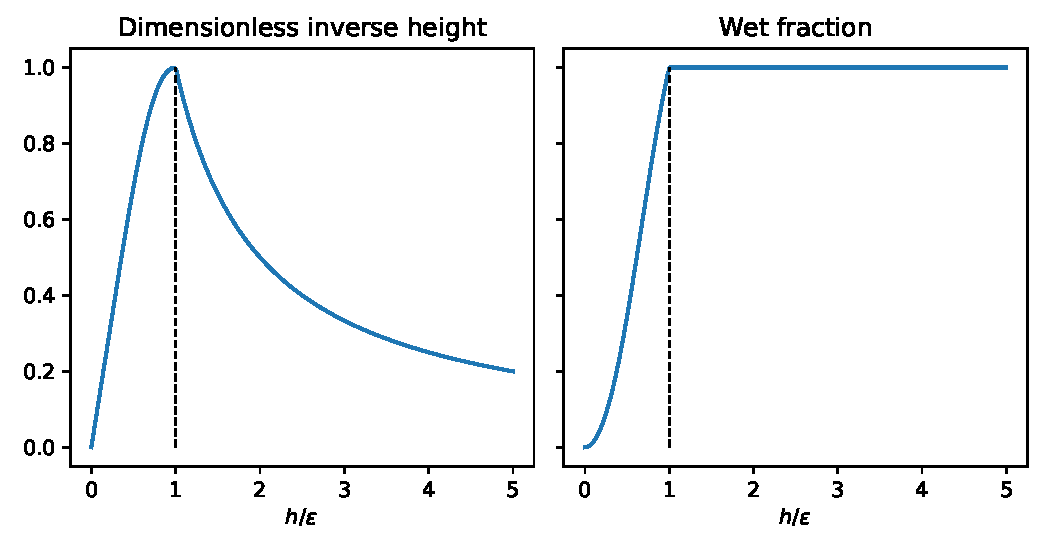
\includegraphics[width=\textwidth]{img/eulerian/inverse_height.pdf}
    \caption{Dimensionless functions to compute the  inverse height and the wet fraction.}
    \label{inverse_heihgt}
\end{figure}


% \paragraph{Partially wet elements}
% At the elements where the shoreline is located, the interpolated water depth will not represent the real water surface.
% Therefore, those elements need a special consideration in order to prevent unrealistic oscillations. Excluding those elements from the computations is equivalent to introduce an artificial barrier, and the inclusion of those elements will incur in a consideration of an extra volume of water.
% We chose to include all the elements in the computation and to modify the balance equations in order to satisfy equilibrium at rest (Figure \ref{partially_dry}). This is achieved by introducing a modified topography
% $z'$ which is obtained imposing the following equilibrium condition:
% \begin{equation}
%     \pder{\eta'}{x_i} = \pder{z'}{x_i} + \pder{h}{x_i} = \mathbf{0}
% \end{equation}

% \begin{figure}
%     \centering
%     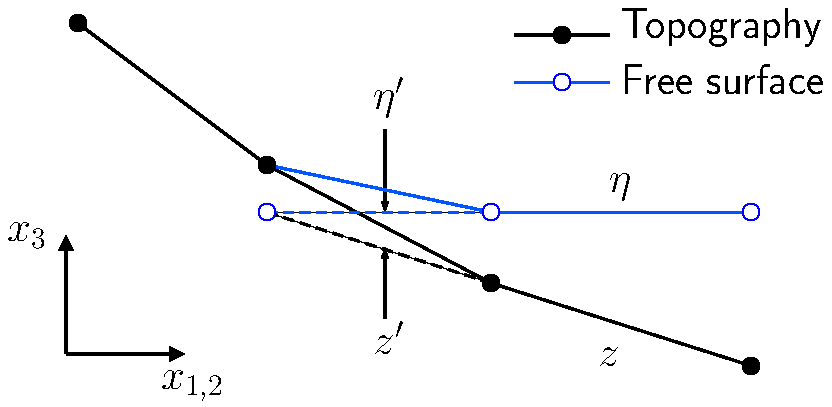
\includegraphics[width=.5\textwidth]{img/fig/partially_dry.pdf}
%     \caption{Dry, wet and partially wet elements in 1D. The dashed line shows the modified topography  and the corresponding free surface.}
%     \label{partially_dry}
% \end{figure}

% Following the idea of \cite{defina2000}, the identification of partially wet elements is done across the definition of a wet fraction function. In this research, instead of modifying the vertical integration of the Navier-Stokes equations, the wet fraction is  defined making use of the pseudo inverse $\hat{h}^{-1}$. The wet fraction $w$ reads:
% \begin{equation}
% w = h\hat{h}^{-1}
% \end{equation}

% The wet fraction function is defined in all the elements -wet, dry and partially dry- and its value goes from $0$ for dry elements to $1$ for wet elements (see Figure \ref{inverse_heihgt})
% This function makes possible to construct the source system vector $\mathbf{T}$ (see equations (\ref{discrete_sw}) and (\ref{discrete_sw_matrices})) with a linear combination between the two topographies as $wz + (1-w)z'$.


\paragraph{Avoiding the singularity of the system matrix}
Since all the elements are included in the computational domain, the last issue to overcome with small water depths are the numerical difficulties stated in Section \ref{equations_sw_lin}.
When there is a null water depth, the theoretical flow rate and velocity are zero. In that point the matrices $\mathbf{A}_i$ are not invertible and the eigenvalues are all equal to zero. In that case, the hyperbolicity property of the system is lost.
In practice, due to spurious oscillations, the flow rate and the velocity may be different from zero. The idea is to freeze the flow and to allow to invert the system matrix adding a diagonal of non zero terms to the momentum equation, i. e.,


\begin{equation}
\mathbf{G} \defeq \mathbf{G} + \xi\,\text{diag}(1, 1, 0)
\end{equation}


The selection of the areas where there is a dry domain is controlled with the wet fraction function and $\xi$ is defined as
\begin{equation}
\xi = k(1-w)
\end{equation}

In our numerical experiments we have chosen $k=10^3$.
The addition of a diagonal matrix remembers the artificial Manning friction proposed in \cite{heniche2000}. This term plays the role of freezing the flow in dry areas.


\paragraph{Mass conservation properties}
The stabilized method proposed is not monotonic and the dry domain model is acting to ensure stability, but it does not provide monotonicity. We note that all the modifications have been done at the momentum balance level. This means that mass is conserved globally by the weak formulation, but the mass sign preservation is not guaranteed.

Both unknowns, water depth and flow rate, are continuous at the dry-wet interface, but its derivatives are discontinuous. Even though the shock capturing scheme can not avoid this kind of oscillations, it will mitigate them, and the order of accuracy will be lost due to the introduction of the non-linear artificial diffusion \cite{badia2014}.





\subsection{Validation}


In this section the linear stabilization is tested. Conceptual examples are presented only to show the consistency of the linear stabilization and the lack of stability if it is not considered. More complex examples which involve shock capturing at some part of the domain are included at the end of the chapter.




\subsubsection{Patch test}


Following Zienkiewicz \cite{zien1}, the patch test has been used as a first verification of convergence. These tests have been developed imposing stationary solutions and obtaining the topography from the primary unknowns. The spatial domain $\Omega$ is a single element $e$.
Since the solution is stationary, the temporal domain is null and the test consist on the verification of zero accelerations.
Then, if the the solution belongs to the basis functions space, the test will pass analytically.
Otherwise, the test will pass asymptotically when the element is refined by subdivision of the domain ($h$-refinement). In that case, even if the element is not passing the test, the patch test is also useful since is checking the correctness of the implementation.

Several exact solutions have been applied to an element with size of $1m$. For the stabilized formulations a stabilization factor $\beta=0.01$ is used. The flux corrected solution depends directly on the stabilized formulation. If the solution belongs to the FE space, the obtained accelerations are less than $10^{-16}$, which is the round-off of machine precision.

\paragraph{Water at rest}
In this case, the free surface gradient and the velocity are zero. Some solutions can be built with that conditions, such as flat and non-flat topography, and bottom friction. In all the cases the accelerations are zero.

\paragraph{Slope in equilibrium}
This family of solutions verify constant water depth and constant velocity. The gravity terms (coming from the slope) are in equilibrium with the bottom friction terms. Several combinations are obtained with different directions of the slope and different Froude numbers, subcritical and supercritical.

\paragraph{Backwater analysis}
Finally, that family of analytical solutions, presents a constant flow rate where the gravity terms are in equilibrium with the bottom friction. But in that case, the primary unknowns do not belong to the FE space, since, either the velocity or the water depth are not linear. This test is passing asymptotically.




\subsubsection{Wave in a channel with a backward step}

The aim of this example is to show that the Galerkin formulation applied to the shallow water equations is unstable and how the present stabilization method can overcome this issue. A calibration of the stabilization parameter is performed to optimize the effect of the stabilization terms in the obtained solution.
We study the propagation of a wave in a channel with a backward step (Figure \ref{step_mesh}) where all the boundaries are slip. The channel depth is 1m. An initial perturbation in the free surface at the left wall generates a wave which travels from 0 to 6s. The initial perturbation reads
\begin{equation}
\eta(t=0) = 0.05\cos(\pi x) \quad \text{if} \quad x<1, \quad \eta=0 \quad \text{otherwise}
\end{equation}


The wave is reflected at the right wall and then faces the step in the opposite direction.
Figure \ref{waves_propagation} shows the propagation of the wave along the channel.
The problem is discretized with a mesh fine enough to test the artificial diffusion added by the stabilization (Figure \ref{step_mesh}). The average element size is $0.06m$ and near the corner the mesh is refined to $0.02m$.
The time step is set automatically to keep a maximum Courant number equal to $1.0$ at every step. The problem is run three times with different algorithmic constants $\beta = 0.001$, $0.01$ and $0.1$. In this example, the shock capturing term is disabled.

\begin{figure}
    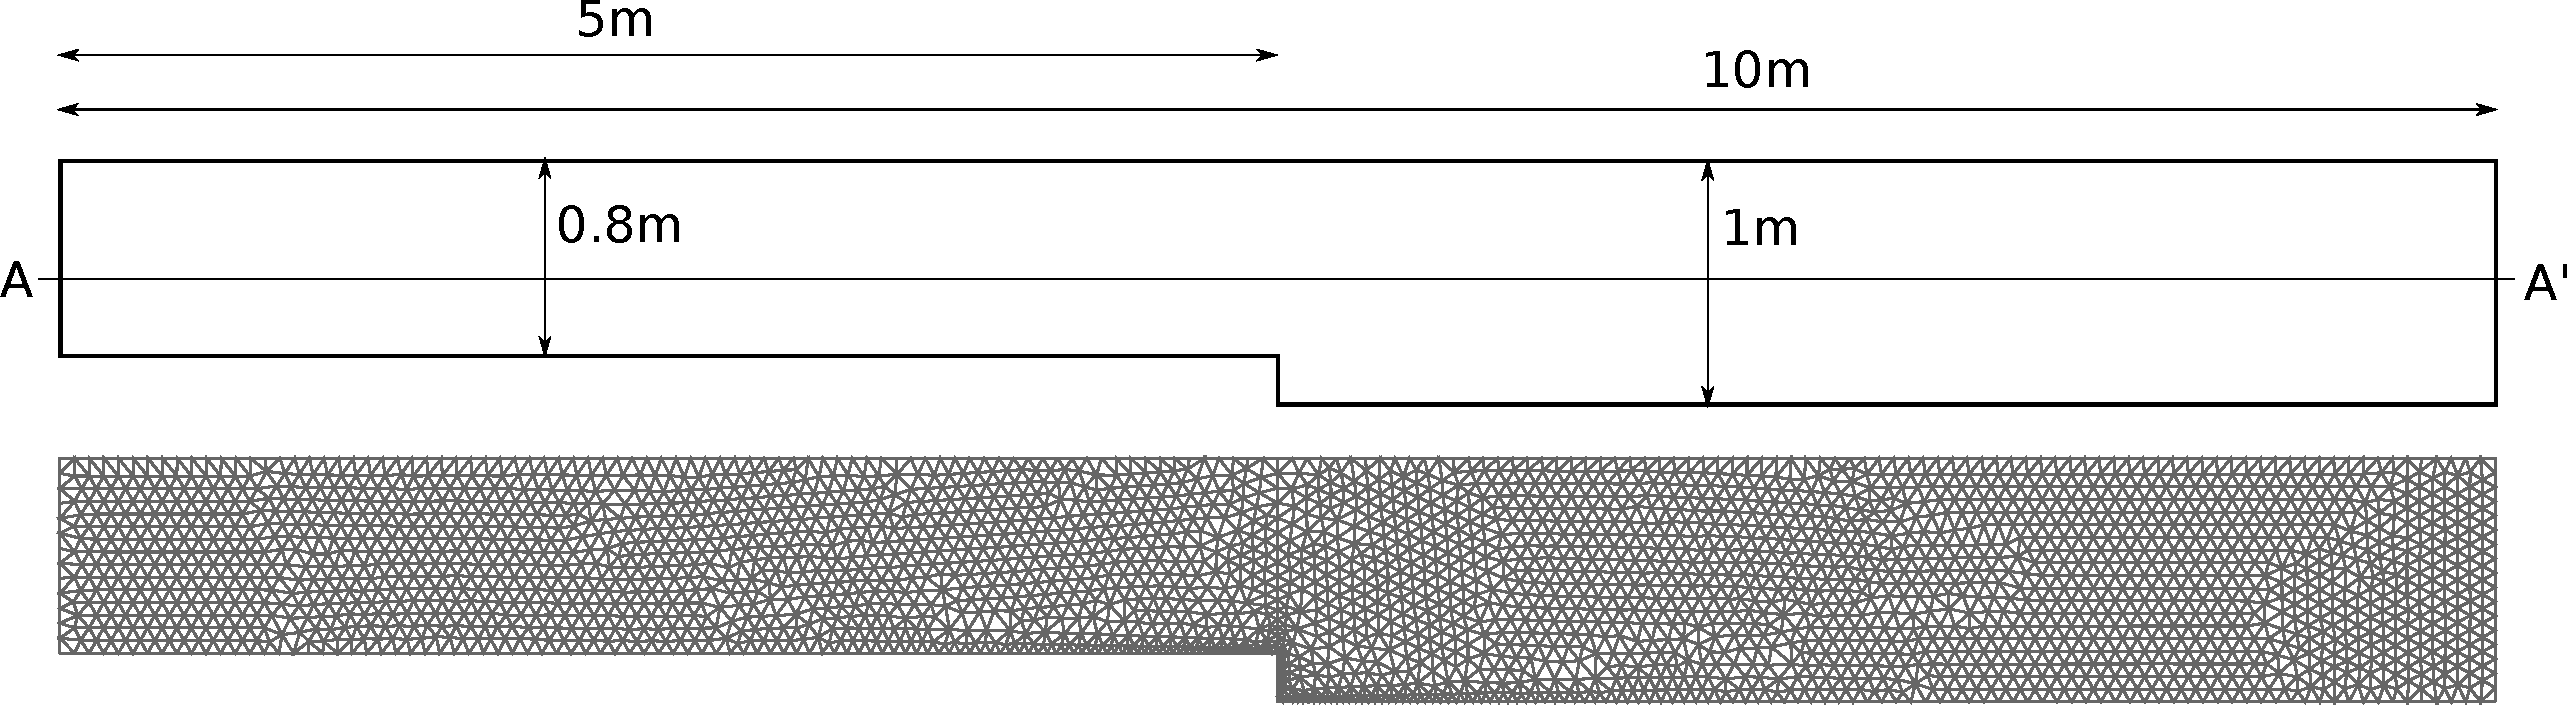
\includegraphics[width=\textwidth]{img/eulerian/step/geometry.pdf}
    \caption{Channel with a backward step. Domain and mesh used in the simulation. All the boundary conditions are slip. The average element size is $0.06m$. Near the obstacle the mesh size is $0.02m$. There are $3.125$ nodes and $5.826$ elements.}
    \label{step_mesh}
\end{figure}

\begin{figure}[H]
\begin{subfigure}{\textwidth}
    \centering
    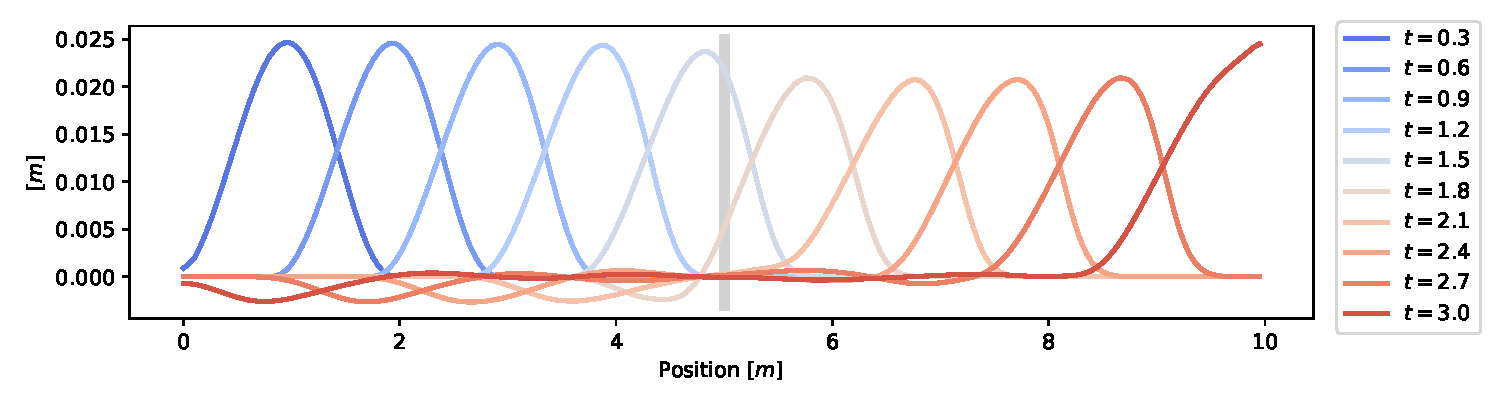
\includegraphics[width=\textwidth]{img/eulerian/step/free_surface_1.pdf}
    \caption{Time from $0$ to $3s$}
\end{subfigure}
\begin{subfigure}{\textwidth}
    \centering
    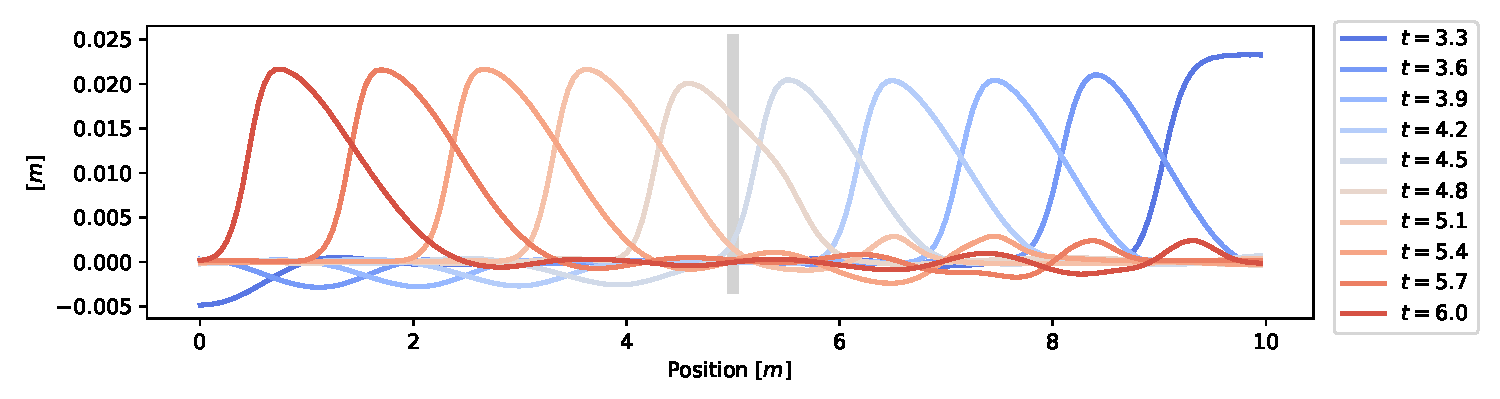
\includegraphics[width=\textwidth]{img/eulerian/step/free_surface_2.pdf}
    \caption{Time from $3$ to $6s$}
\end{subfigure}
\caption{Channel with a backward step. Timestamps of the free surface along the cut AA' from Figure \ref{step_mesh}. (A) The initial perturbation is propagating to the right. (B) Propagation of the reflected wave from right to left.}
\label{waves_propagation}
\end{figure}


The best results are achieved with the intermediate value and it has been fixed for the rest of the examples in this paper.
Figures \ref{stab_parameters_time1} and \ref{stab_parameters_time2} show that the lower value of $\beta$ is not enough to provide stability, while the higher value is over diffusive.

\begin{figure}[H]
\begin{subfigure}{.05\textwidth}
    \caption{}
\end{subfigure}
\begin{minipage}[c]{.94\textwidth}
    
\includegraphics[width=\textwidth]{img/eulerian/step/stab_0.001_time_1.pdf}        
\end{minipage}
\par\medskip
\begin{subfigure}{.05\textwidth}
    \caption{}
\end{subfigure}
\begin{minipage}[c]{.94\textwidth}
    
\includegraphics[width=\textwidth]{img/eulerian/step/stab_0.01_time_1.pdf}        
\end{minipage}
\par\medskip
\begin{subfigure}{.05\textwidth}
    \caption{}
\end{subfigure}
\begin{minipage}[c]{.94\textwidth}
    
\includegraphics[width=\textwidth]{img/eulerian/step/stab_0.1_time_1.pdf}        
\end{minipage}
\caption{Channel with a backward step. Contour plots of the free surface elevation at time $t=1s$ for different stabilization factors. (A) $\beta=0.001$, (B) $\beta=0.01$, (C) $\beta=0.1$}
\label{stab_parameters_time1}
\end{figure}

\begin{figure}[H]
    \begin{subfigure}{.05\textwidth}
        \caption{}
    \end{subfigure}
    \begin{minipage}[c]{.94\textwidth}
        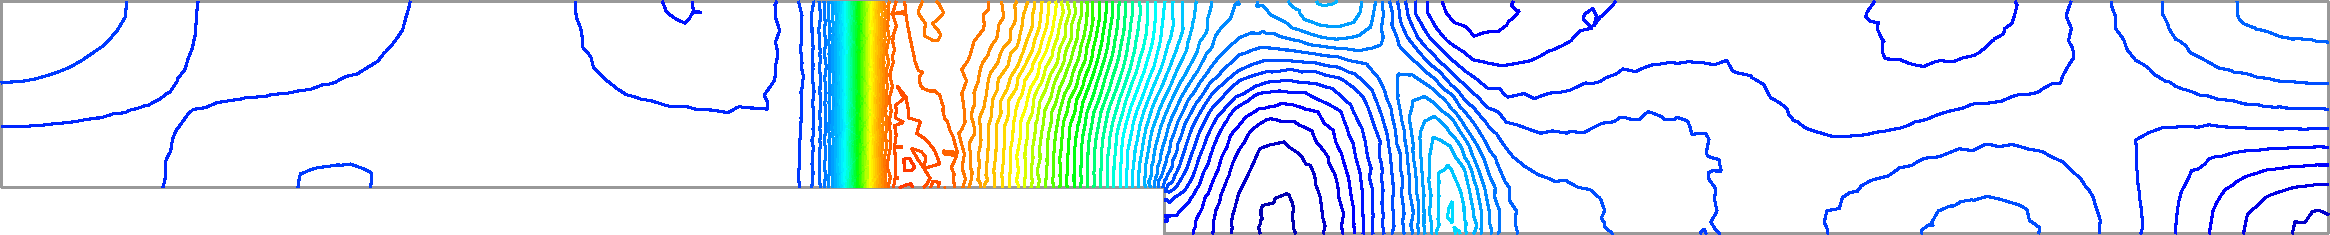
\includegraphics[width=\textwidth]{img/eulerian/step/stab_0.001_time_5.pdf}
    \end{minipage}
    \par\medskip
    \begin{subfigure}{.05\textwidth}
        \caption{}
    \end{subfigure}
    \begin{minipage}[c]{.94\textwidth}
        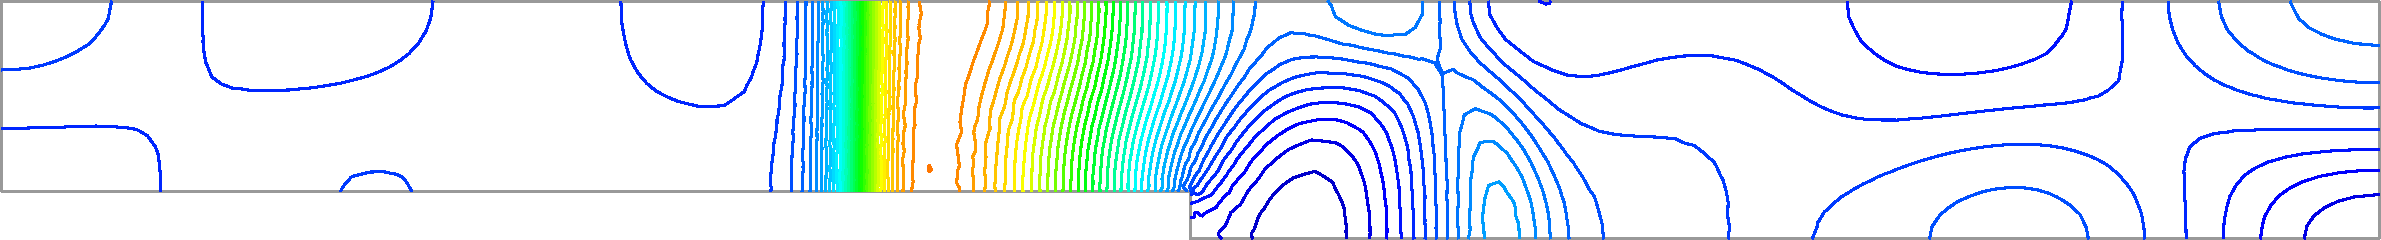
\includegraphics[width=\textwidth]{img/eulerian/step/stab_0.01_time_5.pdf}
    \end{minipage}
    \par\medskip
    \begin{subfigure}{.05\textwidth}
        \caption{}
    \end{subfigure}
    \begin{minipage}[c]{.94\textwidth}
        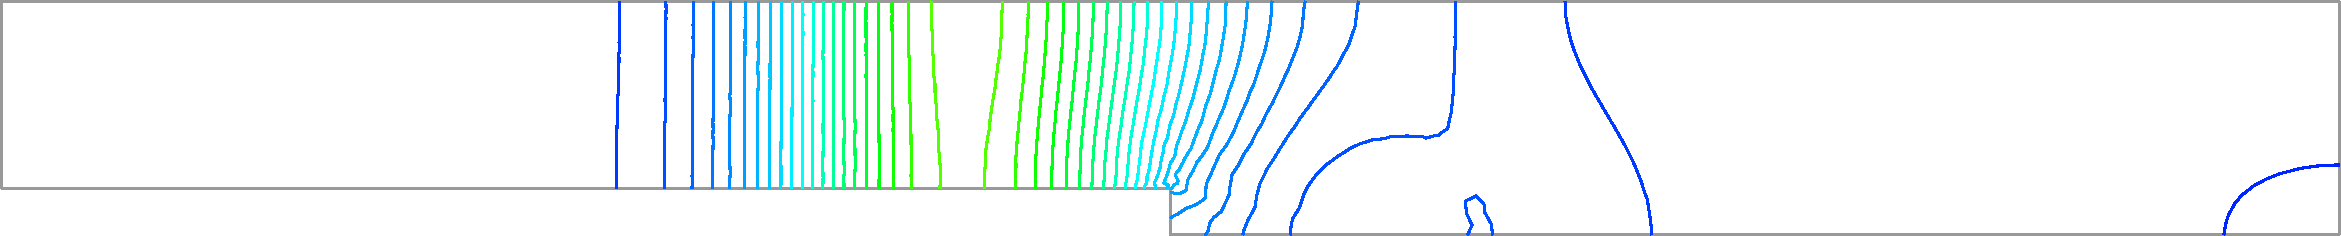
\includegraphics[width=\textwidth]{img/eulerian/step/stab_0.1_time_5.pdf}
    \end{minipage}
\caption{Channel with a backward step. Contour plots of the free surface elevation at time $t=5s$ for different stabilization factors. (A) $\beta=0.001$, (B) $\beta=0.01$, (C) $\beta=0.1$}
\label{stab_parameters_time2}
\end{figure}




%%%%%%%%%%%%%%%%%%%%%%%%%%%%%%%%%%%%%%%%%%%%%%%%%%%%%%%%%%%%%%%%%%%%%%%
%%%%%%%%%%%%%%%%%%%%%%%%%%%%%%%%%%%%%%%%%%%%%%%%%%%%%%%%%%%%%%%%%%%%%%%
%%%%%%%%%%%%%%%%%%%%%%%%%%%%%%%%%%%%%%%%%%%%%%%%%%%%%%%%%%%%%%%%%%%%%%%




\section{The flux corrected algorithm for the shallow water equations}
\label{sec:sw_fc}



As seen in Section \ref{sec:fic_fem_stabilization}, the numerical approximation of hyperbolic systems -convection dominant- exhibit instabilities. Those instabilities are inherent to schemes of order greater than 1 (Godunov barrier theorem \cite{godunov1959}). With the aim of suppressing the spurious oscillations and to extend to stable schemes to higher orders, the flux corrected (FC) algorithms were proposed.
This new family of methods seeks for non oscillatory solutions and also for monotonicity of the numerical solution. At first, the FC algorithms were proposed for structured meshes and explicit time integration schemes \cite{boris1973, book1975}. Generally, they were based for FD algorithms, but rapidly were extended also to Galerkin discretizations and implicit schemes \cite{moller2004, lohner2008ch9}. Even though, the FC transport has not been extended to many applications in the FEM community.


In this section the concept of FC is extended to the SW equations. The linearized equations presented in Chapter \ref{equations} can be understood as a generalization of the scalar transport equations, where the convection operator is extended with a matrix and the scalar unknown is replaced by a vector. This extension is proposed as an alternative to Lagrangian methods (Appendix \ref{lagrangian_sw}), where the shoreline discontinuity is naturally captured. At the same time, it seeks for a better accuracy than the stabilized Eulerian methods (Section \ref{sec:fic_fem_stabilization}):
the introduction of the \emph{shock capturing} leads to a lower convergence order, making them first order. The main purpose to explore the FC algorithm is to make the numerical solution inherit the monotonicity of the physical solution. The water column is a positive property, whereas null water depth means the dry sub-domain.
Tracking the zero isoline properly is of crucial importance to accurately model the wetting and drying processes -floods-. Unfortunately, the zero isoline presents a discontinuity in the unknowns and the hyperbolic property is lost, leading to numerical oscillations and consequently, losing the monotonic property.


The FC algorithm is based on the modification of the resulting matrices from the discrete weak variational. The formulation presented in Section \ref{sec:fic_fem} will be modified in order to enforce it to verify monotonic properties at the discrete level. The subjacent correction acts in such way that all the modifications are conservatives, namely, there is not gain or loss of fluid mass. The original scheme is recovered where the solution is smooth and does no require modifications.


In order to achieve that properties, the low order scheme is constructed through a lumping procedure of the mass matrix and the addition of enough diffusion in order to eliminate the negative entries of the off-diagonal terms. In that way, the construction of the low and high order schemes is performed elementally. On the other hand, the computation of the fluxes and its limiters is computed nodally. Finally, the global assembly is element-wise, as far as the nodes belong to the elements. The fact of recovering the high order scheme with consistent mass matrix is specially interesting to accurately simulate transient problems.




\subsection{Equivalence with pure convection problems}

In a first instance, the FC algorithms where developed for the transport equations as a two stage predictor-corrector algorithm. The correction of the fluxes had a direct relation with the physical fluxes and were evaluated at the edges of the mesh, acting directly to the entries of the global matrix.

Since the pure convection problem is a particular hyperbolic system of conservation law, this algorithm was extended to more complex systems, like the Euler equations. Here we will show the equivalence of the inviscid SW equations with pure convection problems.
The starting point are the linearized SW equations in conservative form (\ref{general_sw_lin}), which are analogue to the hyperbolic euler equations:

\begin{equation}
\pder{\bm\phi}{t} + \bm A_i \pder{\bm\phi}{x_i} = 0
\end{equation}

The matrix $\bm A_i$ is diagonalizable and can be decomposed as $\bm A_i = \bm T_i \bm\Lambda_i \bm T_i^{-1}$. Kuzmin \cite{kuzmin2005b} proposes this transformation for the one dimensional case. In high order dimensions, we can define a vector of transformed unknowns $\bm\Phi_i = \bm T_i^{-1}\bm\phi$ which yields


\begin{equation}
\pder{\bm\Phi_j}{t} + \bm\Lambda_i \pder{\bm\Phi_j}{x_i} = 0
\end{equation}
Since $\bm\Lambda$ is a diagonal matrix, the above expression consists on a set of decoupled convection equations.

\begin{equation}
\pder{\Phi_{jk}}{t} + \Lambda_{ikk} \pder{\Phi_{jk}}{x_i} = 0 , \quad
k = 1:n_b , \quad
i,j = 1:n_d
\end{equation}

In practice, instead of applying the FC concept to the diagonal system, the algorithm will be extended to the original system os equations. The main difficulty which appears when the system is decomposed is that there isn't a unique direction of propagation for each uncoupled unknowns. This is known as the dispersive behavior of the shallow water equations.



\subsection{Flux-corrected algorithm}

The FC algorithm inherits the concept of \emph{limiting} introduced by Boris and Book \cite{boris1973} and was developed by Löhner \cite{lohner2008ch9} and Kuzmin \cite{kuzmin2001}. They also extended the concept of FC to the euler equations \cite{lohner2008ch9, kuzmin2005b}. In more recent developments, the FC technique was applied to the shallow water equations by Ortiz \cite{ortiz2012}. However, Ortiz presents an algorithm with a fully decoupled high and low order schemes. In this section, the FC scheme is applied to the shallow water equations preserving the same discretization for both high and low order schemes. 



\subsubsection{High and low order schemes}

Usually, the high order scheme is a FEM solution, such as a Taylor-Galerkin \cite{lohner2008ch6} or Characteristic Based Split (CBS) \cite{ortiz2012}.
In this work, the high order solution uses the spatial discretization presented in Section \ref{sec:fic_fem} with linear stabilization and without shock capturing. The time integration scheme is the backward differentiation formula from Section \ref{sec:time_integration_bdf}.

\begin{equation} \label{ho}
\mathbf{M}_C\dot{\phi}^{n+1} + \mathbf{K}\phi^{n+1} = \mathbf{q}
\end{equation}
\begin{equation} \label{bdf}
\dot{\phi}^{n+1} = \beta_1\phi^{n+1} + \beta_2\phi^{n} + \beta_3\phi^{n-1}
\end{equation}

where $\phi$ is the vector of the nodal unknowns and $\dot{(\ )}$ denotes the time derivative, $\mathbf{M}_C$ is the consistent mass matrix, $\mathbf{K}$ is the system matrix and $\mathbf{q}$ is the source term. This scheme will be taken as reference for the high order scheme but, as any stabilized and not monotonicity preserving formulation, is not oscillation-free, specially near the wet-dry interface.
%In \cite{ortiz2012} the high order solution is obtained with the CBS algorithm, which was initially proposed by Zienkiewicz and Taylor \cite{zien3}.

The low order solution is obtained from the high order scheme with a mass lumping procedure and adding scalar diffusion to the high order scheme:

\begin{equation} \label{lo}
\mathbf{M}_L\dot{\phi}^{n+1} + \left(\mathbf{K+D}\right)\phi^{n+1} = \mathbf{q}
\end{equation}
\begin{equation} \label{scalar_diffusion}
\mathbf{D} = c_\tau\left(\mathbf{M}_L - \mathbf{M}_C\right)
\end{equation}

The difference between the two systems of equations is the amount of artificial diffusion which ensures monotonicity and can be formally written as

\begin{equation}
\mathbf{P}(\phi^{n+1}, \phi^n) = (\mathbf{M}_L - \mathbf{M}_C)\dot{\phi}^{n+1} - \mathbf{D} \phi^{n+1}
\end{equation}

Following Kuzmin \cite{kuzmin2005a}, one can observe that the anti-diffusion $\mathbf{P}$ can be decomposed into a sum of internodal fluxes $f_{ij}$ where the contribution to node $i$ from the node $j$ is the opposite from $i$ to $j$, that is $f_{ij}=-f_{ji}$. This edge-based approach shows that the quantity added to a node, is subtracted from another node, and the anti-diffusion is conservative. For convenience we will keep the finite element structure. The high order scheme is recovered if the unlimited correction $\mathbf{P}$ is added to the low order scheme.



\subsubsection{Flux correction limiter}

The essentials of the FC method is to switch between the low and high order solutions in an adaptive fashion to satisfy the positivity constraint. The Zalesak limiter is employed to define the amount of anti-diffusion added to the low order solution which at the same time guarantee the positivity constraint for a given variable. The main steps explained above are depicted in Figure \ref{sw_fc_steps}.

The anti-diffusive fluxes are decomposed in those that increase the value and those that decrease it, the increment $\mathbf{P}_i$ is decomposed in a sum of positive and negative contributions

\begin{equation}
P_i = P_i^+ + P_i^- \ , \qquad
P_i^{\pm} = \sum_{j\neq i} \,
_{\min}^{\max} \{0, j_{ij}\}
\end{equation}

While the maximum/minimum admissible increments depends on the solution values at the neighboring nodes that share an element with node $i$

\begin{equation} \label{admissible_increment}
Q_i^\pm =\, _{\min}^{\max}\Delta \phi_{ij}^\pm \ , \qquad
\text{where} \quad \Delta \phi_{ij}^\pm =\, _{\min}^{\max}
\{0, \tilde{\phi}_j - \tilde{\phi}_i\}
\end{equation}

where the $\tilde{(\ )}$ symbol denotes a predictor for the solution at time $t^{n+1}$. In order to prevent the formation of spurious oscillations, the positive/negative anti-diffusive flux should be limited by the following ratio

\begin{equation}
R_i^\pm = \begin{cases}
    \min\{1, Q_i^\pm / P_i^\pm\} & \text{if} P_i^\pm \neq 0 \\
    1 & \text{if} P_i^\pm = 0
\end{cases}
\end{equation}

It is important to note that, in order to preserve mass conservation property, the same limiter should be applied to all the element contributions. So, the most restrictive ratio is chosen:

\begin{equation}
c_e = \min\{R_i^\pm\}\ , \quad \forall \text{node}_i \in \text{element}_e
\end{equation}

% \begin{equation}
% c_e = \begin{cases}
%     \min\{R_i^+\} & \quad \text{if} \quad \sum_i f_i>0 \\
%     \min\{R_i^-\} & \quad \text{if} \quad \sum_i f_i<0
% \end{cases}
% \end{equation}


\begin{figure}
\centering
\begin{subfigure}{.8\textwidth}
    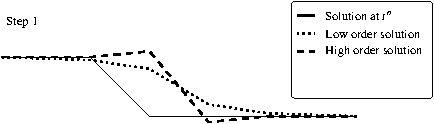
\includegraphics[width=\textwidth]{img/eulerian/fc/fc_step_1.pdf}
    \vspace{1em}
\end{subfigure}
\begin{subfigure}{.8\textwidth}
    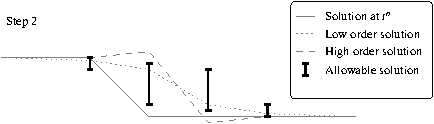
\includegraphics[width=\textwidth]{img/eulerian/fc/fc_step_2.pdf}
    \vspace{1em}
\end{subfigure}
\begin{subfigure}{.8\textwidth}
    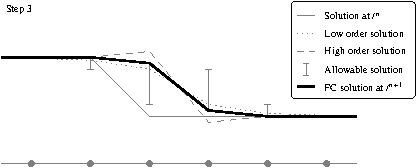
\includegraphics[width=\textwidth]{img/eulerian/fc/fc_step_3.pdf}
\end{subfigure}
\caption{Main steps of the FC algorithm for the computation of the solution at time step $t^{n+1}$.}
\label{sw_fc_steps}
\end{figure}



\subsubsection{Iterative solution}

Since the linearization matrix $A$ depends on the solution at time $t^{n+1}$, the system matrix $K$ needs to be updated at the end of each iteration and the low order algebraic system of equations (\ref{lo}) is rewritten in residual based form

\begin{equation} \label{residual_based}
\left(\beta_0 \mathbf{M}_L + \mathbf{K}^{(m)} + c_\tau\mathbf{D}\right) \Delta\phi^{(m+1)} =
\mathbf{q} - \left(\mathbf{K}^{(m)} + c_\tau\mathbf{D}\right)\phi^{(m)}
-\mathbf{M}_L\dot{\phi}^{(m)}
\end{equation}

where $\phi^{(0)} = \phi^n$. After adding the limited flux correction and substitutions, the system (\ref{residual_based}) yields

\begin{multline}
\left(\beta_0 (c\mathbf{M}_c + (1-c)\mathbf{M}_L)
    + \mathbf{K}^{(m)} + c_\tau(1-c)\mathbf{D}\right) \Delta\phi^{(m+1)} = \\
\mathbf{q} -\left( \mathbf{K}^{(m)} + c_\tau(1-c)\mathbf{D} \right) \phi^{(m)}
    - \left(c\mathbf{M}_c + (1-c)\mathbf{M}_L \right) \dot{\phi}^{(m)}
\end{multline}




NOTE: the displacement or residual criteria does not converge if the $c_i$ limiter vary along the iterations $(m)$. There are some alternatives to overcome this issue:
\begin{itemize}
    \item to use a constant $c_i$, obtained from the first iteration. This solution may not be optimal and possibly does not preserve monotonicity;
    \item to use a semi-implicit time integration scheme which defines the predictor $\tilde{\phi}$ see equation (\ref{admissible_increment});
    \item to define an incremental limiting, this seems to be the most accurate scheme, even though it is more diffusive than the presented one.
\end{itemize}



\subsubsection{Limiting a set of equations and variable transformation}

The presented limiting is based on the monotonicity requirements for scalar convection, however, the coupling of the shallow water equations require a synchronized limiting for the correction factors. It is commonly accepted that for coupled systems of equations the flux limiter taken the most restrictive among the set of variables $c_i^+ = \min\{c_{ik}^+\}$ and $c_i^- = \min\{c_{ik}^-\}$. There are the following strategies to compute the set of limiters $c_{ik}^\pm$:

\begin{itemize}
    \item flux limiting in terms of the independent variables $h, \mathbf{q}$;
    \item flux limiting based on several indicators as the total energy, water pressure or maximum eigenvalue;
    \item transformation of the variables into characteristic variables in order to obtain a set of decoupled system of equations where the principles of the flux correction for pure convection can be applied.
\end{itemize}

In omission of source terms, equation (\ref{residual}) can be multiplied by the $\mathbf{T}_i$ base of eigenvectors and transformed into a set of decoupled pure convection problems

\begin{equation}
\pder{\Phi_{jk}}{t} + \Lambda_{ikk} \pder{\Phi_{jk}}{x_i} = 0 , \quad
k = 1:\text{dim}+1 , \quad
i,j = 1:\text{dim}
\end{equation}

This transformation should be computed locally at each node and depends on the current solution at time $t^{n+1}$. However, for the two dimensional case, the set of variables $\phi$ is transformed in a two dimensional vector of variables $\Phi_i$, hence the scalar transport correction techniques should be extended to vectorial transport.


The difficulties presented by the variables transformation lead to the consideration if it is worth computing them rather that directly using the independent variables or an indicator. The limiting based on the independent variables was the choice presented in \cite{lohner2008ch9} and it is the approach followed in this study.

In section \ref{sec:examples} the accuracy of the flux corrected algorithm will be analyzed and compared against the residual-based formulation. In the following section an alternative to the flux corrected algorithm is explored.






\section{Quasi monotonicity preserving formulations}
\label{sec:monotonic}



The scope of this section is to recover the stabilized formulation from Section \ref{sec:fic_fem_stabilization} and apply some of the monotonic properties from Section \ref{sec:sw_fc}. Authors as Burman and Badia demonstrated that, under certain situations, stabilized monotonic solutions can be obtained (see \cite{burman2007, burman2010, badia2014} for example).
Following these authors, the stabilizations can be classified into residual and projections-based. In the first category, we can find some stabilization methods, such as SUPG, GLS, VMS or FIC, based on the proposals of Hughes et al \cite{brooks1982,hughes1989,hughes1995}. This is the option followed in Section (\ref{sec:fic_fem_stabilization}). 
In the second group, Codina proposed the Orthogonal Sub Scales (OSS) method \cite{codina2000}. The inconvenient of this method is the introduction of a global projection to solve the sub-scales. As an alternative, methods with local projection stabilization (LPS) appeared, see (\cite{braack2006,badia2012,badia2014,burman2015,matthies2007})). The main difference among this methods and the residual-based is tha they introduce only the terms which guarantee stability.

Nevertheless, the stabilizations are not a sufficient condition to ensure oscillation-free solutions near discontinuities as they are not monotonicity preserving. The monotonicity can be verified through the well-known shock-capturing methods.
Those family of methods present a good global convergence and introduce non-linear viscosity around discontinuities \cite{Johnson1990}.
Once again, there are two families for the design of non-linear viscosity: the residual-based methods and the gradient jump methods.

Taking into consideration both the accuracy and convergence, the best option seems to be the combination of linear stabilization and residual-based shock capturing. It presents a good global convergence and, only where it is needed, the order of convergence is sacrificed with the introduction of artificial viscosity. Nevertheless, this choice of stabilization leads to a scheme which does not guarantee the monotonic properties of the system.

Burman proved that, under certain conditions, monotonicity can be achieved using a nonlinear viscosity based on the variation of the gradient \cite{burman2007}. However, it is important to consider that an arbitrary combination of methods can lead to the loss of the monotonic properties offered by one of the two methods \cite{badia2014}.




\subsection{Shock capturing}


Traditionally, the most used method to eliminate the spurious oscillations near discontinuities is the local artificial viscosity. Considering a discretization of finite elements $\langle\bm{\omega}, \mathbf{r}\rangle$ where $\langle \cdot,\cdot \rangle$ is the discrete counterpart of the variational principle, a non linear stabilization can be expressed as
\begin{equation}
    \langle\bm{\omega}, \mathbf{r}\rangle + s(\bm{\omega}, \bm{\phi}) = 0
\end{equation}
where
\begin{equation}
    s(\bm{\omega}, \bm{\phi}) = \langle \epsilon(\bm\phi) \nabla\bm\omega , \nabla\bm\phi \rangle
\end{equation}
and the non linear viscosity $\epsilon(\bm\phi)$ is sufficiently large near the discontinuities in order to mitigate oscillations.
In the framework of the FEM, the design of $\epsilon(\bm\phi)$ can be residual-based (RV), gradient jump based (GJV) or entropy based (EV) \cite{guermond2011}.
Usually, RV have been combined with linear stabilization and EV have been applied alone. The argument that justify the choice of using EV without stabilization is that linear stabilization acts as an hyper-viscosity term eliminating DMP property.

GJV methods introduce the concept of jump $[[v]]_a$ and average $\ldbrace v \rdbrace_a$ of a property $v$ in a point $a$ belonging to the boundary of an element. Being $\mathbf{n}$ the normal vector to the boundary, there are the following definitions
\begin{subequations}
\begin{equation}
    [[v]]_a =   \lim_{\epsilon\rightarrow 0} (
        v(\mathbf{a}+\epsilon \mathbf{n})\cdot\mathbf{n}
        - v(\mathbf{a}+\epsilon \mathbf{n})\cdot\mathbf{n})
\end{equation}
\begin{equation}
    \ldbrace v \rdbrace_a = \frac{1}{2}  \lim_{\epsilon\rightarrow 0} (
        v(\mathbf{a}+\epsilon \mathbf{n})\cdot\mathbf{n}
        + v(\mathbf{a}+\epsilon \mathbf{n})\cdot\mathbf{n})
\end{equation}
\end{subequations}

Burman proposed in \cite{burman2007} a shock capturing with monotonic properties for the Burgers equation in 1D. Badia extended that method to multiple dimensions for the scalar transport in \cite{badia2014}. Here, the proposed formulation for scalar transport is applied to the SW equations, using the water depth as the transported property.
The formulation proposed in \cite{badia2014} is defined by the following artificial viscosity for each element $e$:
\begin{equation}
    \epsilon(h)_e = c_{gjv} l_e \Vert \mathbf{A}\Vert_{L^{\inf}_e}\max_{b\in e} \left[
        \frac{
            \int_b|\nabla h\cdot\mathbf{n}|d\sigma
        }{
            \int_b\Vert\nabla h\Vert d\sigma
        }
        \left(
            \frac{
                \int_b|[[\nabla h]]|d\sigma
            }{
                \int_b\ldbrace|\nabla h\cdot\mathbf{n}|\rdbrace d\sigma
            }
        \right)^q
    \right] 
\end{equation}

The parameter $c_{gjv}$ is an algorithmic constant. The original expression depends on some mesh shape parameters and the angles of the element. In practice $c_{gjv}=\frac{1}{2}$ is chosen, this expression coincides with the minimum value to guarantee monotonicity in 1D. Nevertheless, the monotonicity is lost in 2D. It is not surprising to lose monotonicity, since that property is even lost for the pure diffusion equation. Even though, it exhibits an optimal behavior.





%%%%%%%%%%%%%%%%%%%%%%%%%%%%%%%%%%%%%%%%%%%%%%%%%%%%%%%%%%%%%%%%%%%
%%%%%%%%%%%%%%%%%%%%%%%%%%%%%%%%%%%%%%%%%%%%%%%%%%%%%%%%%%%%%%%%%%%
%%%%%%%%%%%%%%%%%%%%%%%%%%%%%%%%%%%%%%%%%%%%%%%%%%%%%%%%%%%%%%%%%%%




\section{Examples}
\label{sec:examples}

%The FIC-FEM formulation presented has been implemented in KratosMultiphysics \cite{dadvand2010, dadvand2013}, an open source framework of numerical methods written in C++.
In this section we present four different examples. Three of them are oriented to verify a single aspect of the procedure explained in this research, the global stabilization, the shock capturing technique and the dry-wet interface.
The last one is devoted to test all the capabilities of the formulation in a practical case for which experimental data is available.



\subsection{Oscillation in a parabolic basin}
\label{sec:examples:parabola}

This is a classical benchmark oriented to test the accuracy of the location of the moving boundary. The topography follows a parabolic profile and the water body oscillates on it. The initial configuration corresponds to zero velocity but the free surface is in a non horizontal plane. Given the parabolic profile of the topography, exists an analytical solution for the oscillatory problem and the free surface elevation remains planar. Details about the derivation of the analytical solution can be found in the compilation made by Delestre et al. in \cite{delestre2013}.

The spatial domain $\Omega$ is defined in the interval $[0,L]\times[0,1]m$ where $L=10m$ and all the boundaries are reflective ($\mathbf{u}\cdot\mathbf{n} = 0$). The topography is given by the following expression
\begin{equation} \label{eq:parabola:topography}
z(x,y) = h_0 \left(\frac{1}{a^2}\left(x - \frac{L}{2}\right)^2 - 1\right)
\end{equation}
The primitive variables are defined by
\begin{subequations} \label{eq:parabola:variables}
\begin{align}
h(x,y) &=
\begin{cases}
-h_0\left(\left(\frac{1}{a}\left(x - \frac{L}{2}\right) + \frac{1}{2a}\cos(2Bt)\right)^2 - 1\right)
\quad &\text{if} \ x_1(t) < x < x_2(t) \\
0 \quad &\text{otherwise}
\end{cases} \\
\mathbf{u}(x,y) &=
\begin{cases}
(B,0)\sin(2Bt) \quad &\text{if} \ x_1(t) < x < x_2(t) \\
(0,0) \quad &\text{otherwise}
\end{cases}
\end{align}
\end{subequations}
where $B=\sqrt{2gh_0}/2a$, and $x_1$, $x_2$ are time dependent functions which define the location of the dry-wet interface:
\begin{equation}
\begin{split}
x_1(t) = -\frac{1}{2}\cos(2Bt) - a + \frac{L}{2} \\
x_2(t) = -\frac{1}{2}\cos(2Bt) + a + \frac{L}{2}
\end{split}
\end{equation}
In that example the selected parameters are $h_0=1m$ and $a=1m$.


The domain $\Omega$ is discretized using several meshes in order to perform a convergence analysis. The meshes employed are listed in Table \ref{parabola_convergence_tab}. Figure \ref{parabola_mesh} shows one of the intermediate mesh. Once the simulation begins, the water starts to oscillate on the parabolic basin and the velocity field is constant on the spatial domain, while follows a periodic function respect to the time.

\begin{figure}
    
\includegraphics[width=\textwidth]{img/eulerian/par/mesh_0.1.pdf}
    \caption{Parabolic basin. One of the meshes used in the analysis. The element size is $0.1m$.}
    \label{parabola_mesh}
\end{figure}


A cut along the mesh is depicted in Figure \ref{parabola_graphic} showing the free surface, the velocity and the location of the shoreline.
Since the shoreline is moving, several problems may arise, such as the stability of the wetting or drying element or capturing the discontinuity of the velocity. Fortunately, the velocity is not a a degree of freedom and this will help to avoid spurious oscillations in the vicinity of the shoreline.



\begin{table} [htb]
    \centering
    \begin{tabular}{>{\small}rcccc} \hline
    $n_{nodes}$ & $\Delta x$ & $\Delta t$ & CFL & $L_2(e_{rel})$ \\ \hline
205 & 0.25 & 0.008 & 0.5 & 0.24 \\
1,111 & 0.1 & 0.003 & 0.5 & 0.064 \\
4,221 & 0.05 & 0.002 & 0.5 & 0.023 \\
11,356 & 0.03 & 0.001 & 0.5 & 0.013 \\
101,101 & 0.01 & 0.0003 & 0.5 & 0.0049 \\
    \hline
    \end{tabular}
    \caption{Parabolic basin. Convergence error for the water height.}
    \label{parabola_convergence_tab}
\end{table}

\begin{figure}[H]
\begin{subfigure}{\textwidth}
    \centering
    Time $t=0.5s$
    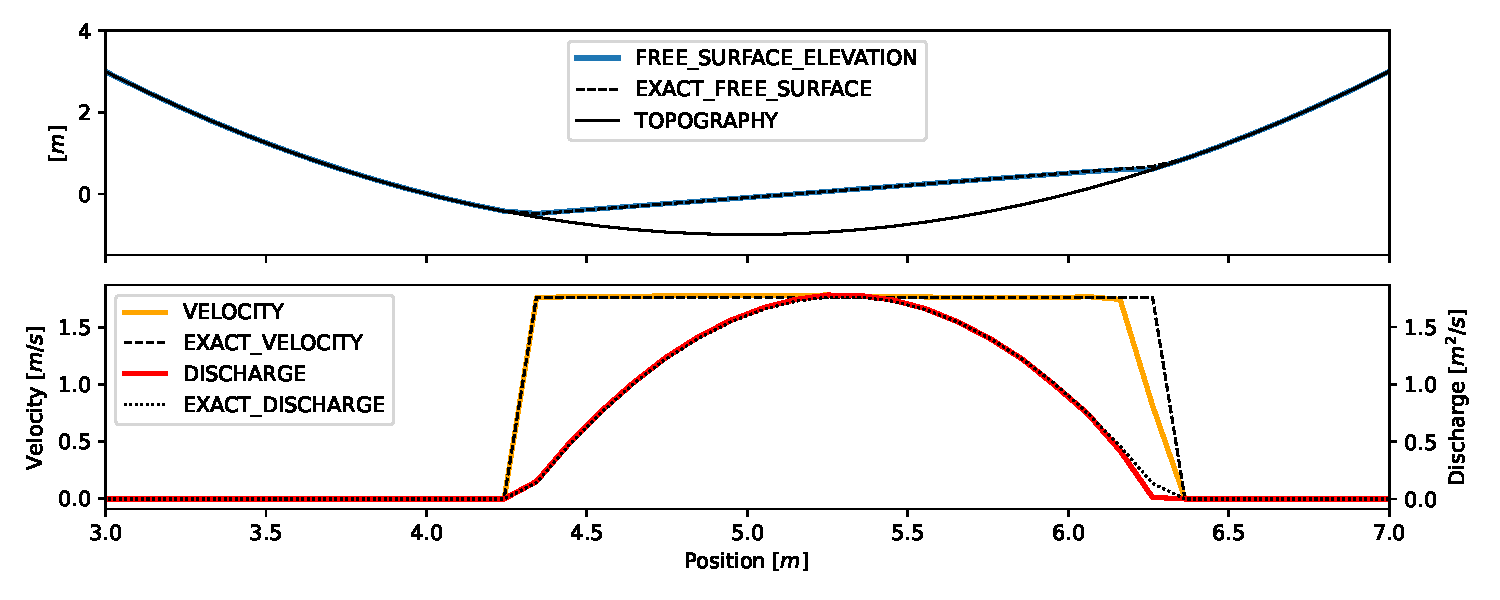
\includegraphics[width=\textwidth]{img/eulerian/par/parabola_t0.5.pdf}
\end{subfigure}
\par\medskip
\begin{subfigure}{\textwidth}
    \centering
    Time $t=1s$
    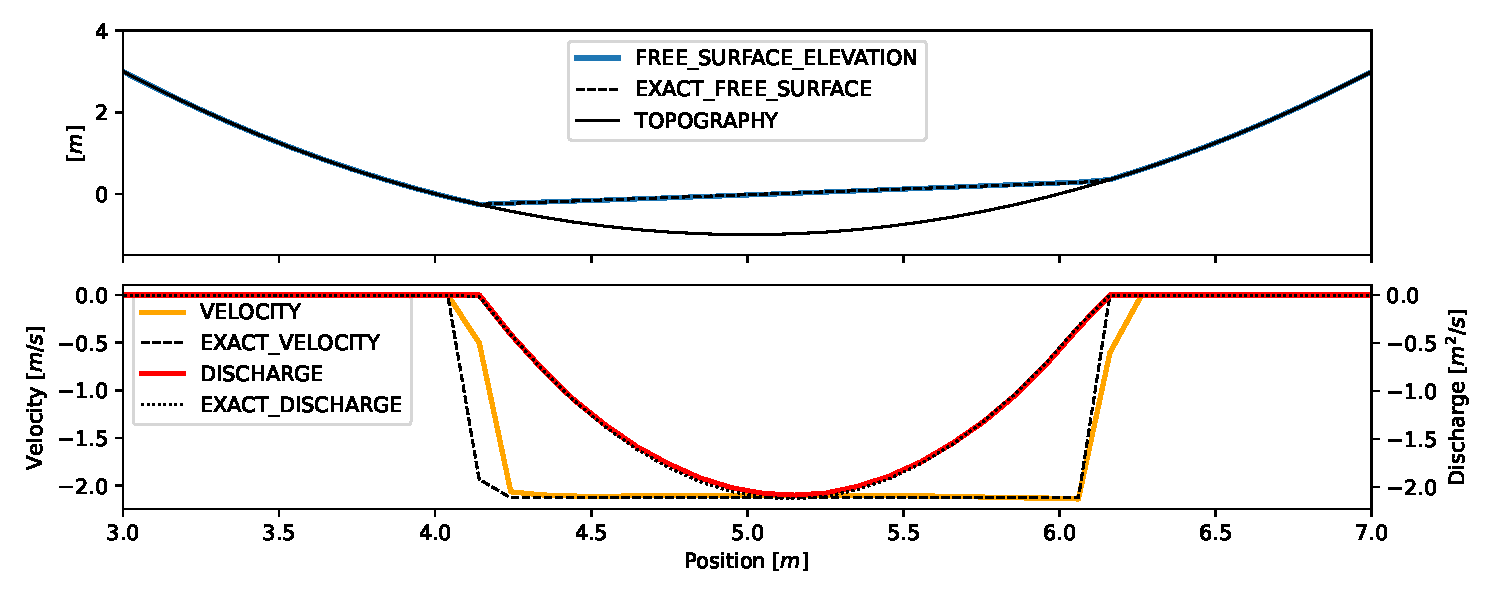
\includegraphics[width=\textwidth]{img/eulerian/par/parabola_t1.0.pdf}
\end{subfigure}
\caption{Parabolic basin. Cuts along the mesh of size $0.03m$ at different times. There are 333 nodes on the cut.}
\label{parabola_graphic}
\end{figure}


A global representation of the solution at time $t=1s$ is presented in Figure \ref{parabola_results}.
In that case the finest mesh ($\Delta x=0.01m$) has been used, for visualization purpose the discretization is not shown. As expected, there is no variation on the results in the transversal section.


\begin{figure}[H]
    \begin{subfigure}{.05\textwidth}
        \caption{}
    \end{subfigure}
    \begin{minipage}[c]{.94\textwidth}
        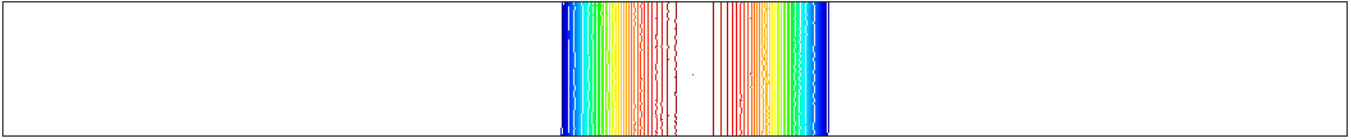
\includegraphics[width=\textwidth]{img/eulerian/par/height.png}
    \end{minipage}
\par\medskip
    \begin{subfigure}{.05\textwidth}
        \caption{}
    \end{subfigure}
    \begin{minipage}[c]{.94\textwidth}
        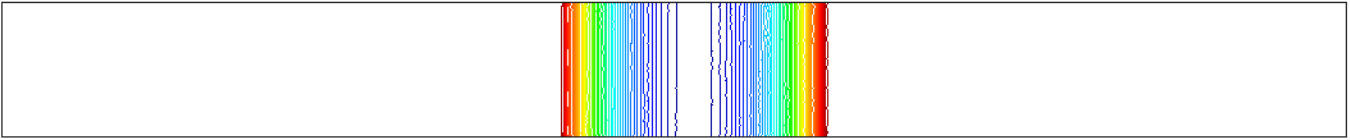
\includegraphics[width=\textwidth]{img/eulerian/par/momentum.png}
    \end{minipage}
\par\medskip
    \begin{subfigure}{.05\textwidth}
        \caption{}
    \end{subfigure}
    \begin{minipage}[c]{.94\textwidth}
        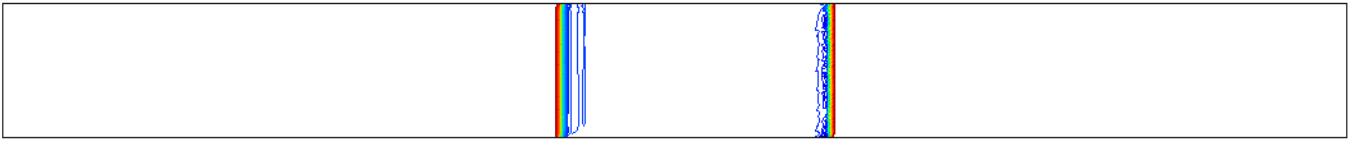
\includegraphics[width=\textwidth]{img/eulerian/par/velocity.png}
    \end{minipage}
\caption{Parabolic basin. Contour lines with the fine mesh of size $0.01m$ at time $t=1s$. (A) Water height, (B) x-discharge and (C) x-velocity. There is no legend for simplicity.}
\label{parabola_results}
\end{figure}





\paragraph{Combination of linear with non linear stabilization}


The main problem of linear stabilizations is the loss of the monotonic properties which may be provided by nonlinear stabilizations. For that reason, in \cite{guermond2011} is proposed to use a nonlinear stabilization alone. This is the case of EV.
However, the use of nonlinear stabilization alone, may lead to unwanted results. The most common undesired results are such as terracing near the boundaries \cite{lohner2008ch9,kuzmin2005b} and mesh-dependent diffusivity \cite{badia2014}.

It is known that the combination of GJV with SUPG or FIC is not monotonicity preserving. However, the monotonic properties can be improved if it is compared against a standard RV method. The convergence of the presented methods is compared in Figure \ref{parabola_convergence}.



\begin{figure} [htp]
    \centering
    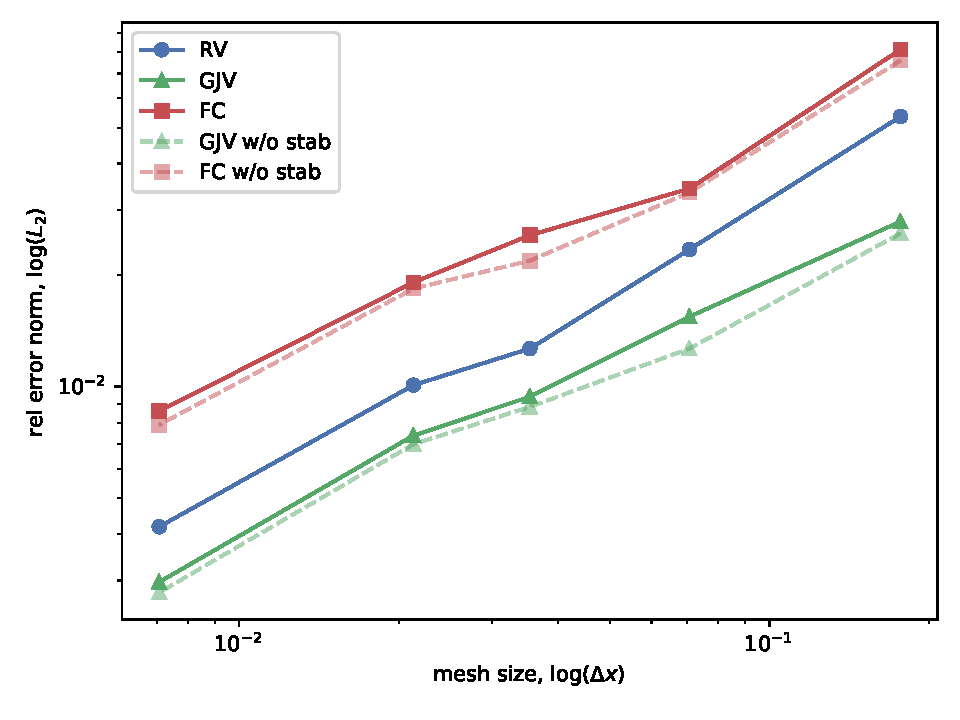
\includegraphics[width=.8\textwidth]{img/eulerian/par/conv_1.pdf}
    \caption{Parabolic basin. Convergence graph.}
    \label{parabola_convergence}   
\end{figure}



A mass conservation test is performed with the mesh of size $0.05m$ in a simulation of $5s$. The results are presented in Figure \ref{parabola_mass}. The integration of the mass is performed over all the domain and over the wet domain. The wet domain is identified with the wet fraction, requiring that it is equal to $1$. Since the presented schemes are not mass sign preserving, the wet mass can not be equal to the total mass and a small fraction is lost from the wet domain. The loss depends on the element size and presents an oscillatory behavior inherent of the method.

Regarding the different non linear stabilizations, it is clear that none of the presented methods is able to ensure monotonicity. Nevertheless, the gradient jump viscosity method reduces the magnitude of the oscillations. Another interesting feature is that the maximum oscillation is bounded and does not increase during the natural oscillations of the sloshing. The flux-corrected algorithm presents the maximum spurious oscillations.


\begin{figure}[H]
    \centering
    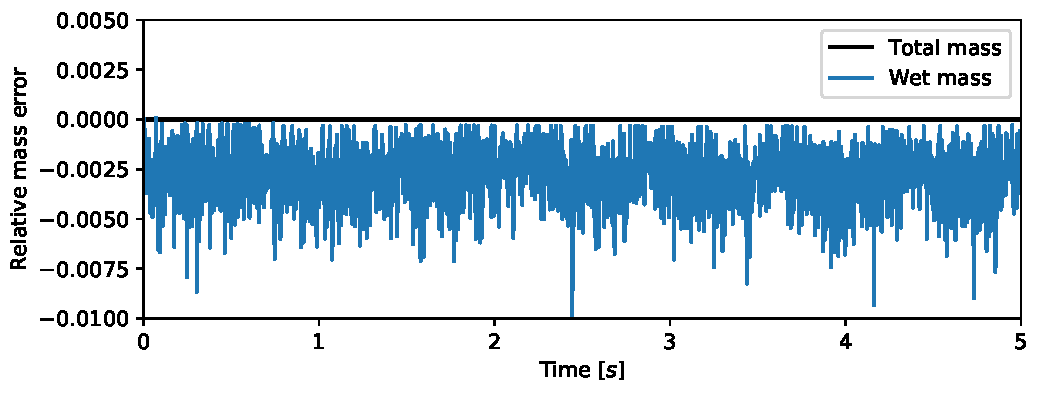
\includegraphics[width=.95\textwidth]{img/eulerian/par/mass_conservation}
    \caption{Parabolic basin. Mass conservation error. The element size used in this simulation is $0.05m$.}
    \label{parabola_mass}
\end{figure}





\subsection{Short channel with smooth transition and shock}
\label{sec:examples:shock}


The second example consists on a benchmark based on the Mac Donald's type solutions \cite{macdonald1997}. The analytical solution can be found in the compilation which was referenced in the previous example \cite{delestre2013}. This test presents a channel with a steady state solution. There is a subcritical inlet and a transcritical flow is produced. The outlet is also subcritical and then a shock is generated at $\sfrac{2}{3}$ of the channel. The aim of this example is to evaluate the shock capturing technique presented and the correct location of the hydraulic jump, which depends on the bottom friction law.

Here we will consider the 1D shallow water equations without diffusion and only with Manning bottom friction as source term. A steady state solution satisfies $\pder{q}{x}=0$ and Equation (\ref{general_sw}) reduces to
\begin{equation} \label{steady_state}
\pder{z}{x} = \left(\frac{v^2}{gh}-1\right) \pder{h}{x} - n^2\frac{\abs{v}v}{h^{\sfrac{4}{3}}}
\end{equation}
This relation allows to integrate the topography given an analytical expression for the water height. Another approach in hydraulics is to consider a given discharge and topography and integrate the water height using Equation (\ref{steady_state}). Following both approaches exact solutions can be obtained. Since this expression involves the bottom friction, we can verify if the friction term is correctly coded in order to satisfy the steady state.

For this benchmark we have considered the domain defined by the spatial domain $[0,100]\times[0,5]$ which is a channel of $100m$ length and $5m$ width (Figure \ref{chanel_geometry}), and the following boundary conditions:
\begin{equation}
\begin{split}
    q_x = 2\ \text{m/s} \quad &\text{in} \quad \Gamma_{upstream} \\
    h = h_{ex}(100) \quad &\text{in} \quad \Gamma_{downstream} \\
    q_y = 0 \quad &\text{in} \quad \Gamma_{walls}
\end{split}
\end{equation}

The problem is initialized with the following values:
\begin{equation}
\begin{split}
    h(x,0) &= \max(h_{ex}(100) - z(x), h_{ex}(0)) \\
    \mathbf{q}(x,0) &= \mathbf{0}
\end{split}
\end{equation}


The Manning coefficient is $0.0328\ \text{m}^{-1/3}\text{s}$ and the water height $h_{ex}(x)$ is a piecewise function defined in \cite{delestre2013}. The discontinuity of the water height function is located at $x=200/3m$ and defines the hydraulic jump. The expression of the stationary exact water depth is:
\begin{equation} \label{jump_height_definition}
    h_{ex} = \begin{cases}
        \left(\frac{4}{g}\right)^\frac{1}{3} \left(\frac{4}{3} - \frac{x}{L}\right) - \frac{9x}{10L}
            \left(\frac{x}{L} - \frac{2}{3}\right) \, ,\ \text{for} \ x < \frac{2L}{3}\\
        \left(\frac{4}{g}\right)^\frac{1}{3} \left(
              a_1 \left(\frac{x}{L} - \frac{2}{3}\right)^4
            + a_1 \left(\frac{x}{L} - \frac{2}{3}\right)^3
            - a_2 \left(\frac{x}{L} - \frac{2}{3}\right)^2 \right. \\ \left. \qquad\qquad\qquad\qquad
            + a_3 \left(\frac{x}{L} - \frac{2}{3}\right)
            + a_4
        \right) \, ,\ \text{for} \ x \geq \frac{2L}{3}
    \end{cases}
\end{equation}
where $a_1=0.674202m$, $a_2=21.7112m$, $a_3=14.492m$, $a_4=1.4305m$ and $L=100m$. The topography is obtained by a numerical integration using the fourth order Runge Kutta method.

As in the previous example, several meshes are employed and a convergence analysis is performed (Figure \ref{hydraulic_jump_convergence}). The shock capturing parameter is $\alpha=1.0$ and we will study the accuracy of the hydraulic jump. 
Given the initial conditions, the hydraulic jump is generated between the first $50$ and $80s$. The overall error is computed at time $t=200s$, in order to ensure the stationary state is achieved.
The table from Figure \ref{hydraulic_jump_convergence} shows the error of the $x$-discharge over all the domain using the $L_2$ norm.

Results from different meshes are compared in Figures \ref{mac_donald_shock_graph_5} and \ref{mac_donald_shock_graph_2}. The oscillations are reduced with the finer mesh (Figure \ref{mac_donald_shock_graph_2}), but there is a peak on the discharge at the location of the shock. This peak is initiated because the momentum balance includes the gradient of the total water depth, and the analytical gradient is a Dirac delta function.

\begin{figure} [ht]
    
\includegraphics[width=\textwidth]{img/eulerian/jump/sketch.pdf}
    \caption{Short channel. Geometry of the channel. The vertical line shows the position of the hydraulic jump.}
    \label{chanel_geometry}
\end{figure}


\begin{figure} [htb]
    \centering
    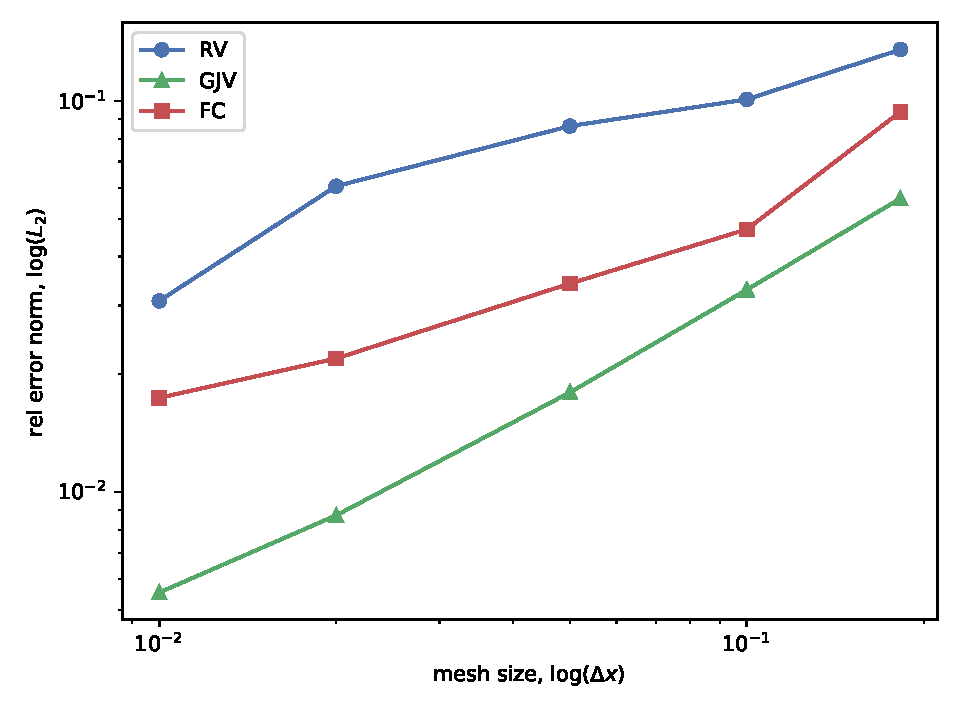
\includegraphics[width=.8\textwidth]{img/eulerian/jump/momentum_convergence.pdf}
    \caption{Short channel. Convergence graph for the $x$-discharge.}
    \label{hydraulic_jump_convergence}
\end{figure}

\begin{table}
    \centering
    \begin{tabular}{>{\small}rcccc} \hline
    $n_{nodes}$ & $\Delta x$ & $\Delta t$ & CFL   & $L_2(e_{rel})$ \\ \hline
    204         &        2.0 &      0.005 & 0.016 & 0.177 \\
    606         &        1.0 &      0.005 & 0.031 & 0.138 \\
    2211        &        0.5 &      0.005 & 0.062 & 0.088 \\
    13026       &        0.2 &      0.005 & 0.15  & 0.041 \\ \hline
    \end{tabular}
    \caption{Short channel. Error for the $x$-discharge.}
    \label{hydraulic_jump_convergence_tab}
\end{table}


\begin{figure}
    \begin{subfigure}[b]{\textwidth}
        \centering
        \caption{Mesh size $0.5m$}
        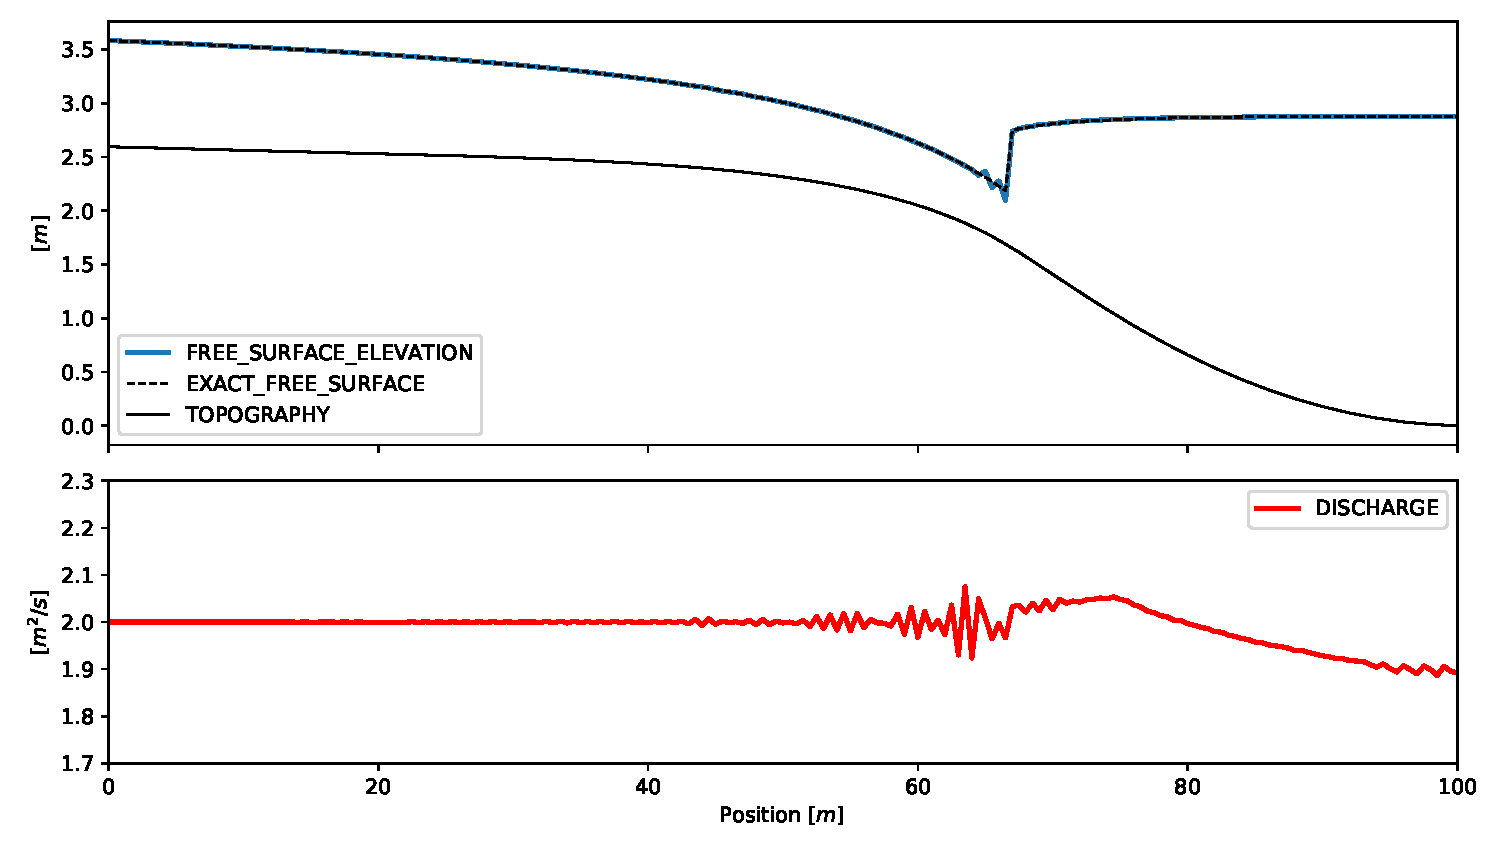
\includegraphics[width=\textwidth]{img/eulerian/jump/mesh_0.5.pdf}
        \label{mac_donald_shock_graph_5}
    \end{subfigure}
    \begin{subfigure}[b]{\textwidth}
        \centering
        \caption{Mesh size $0.2m$}
        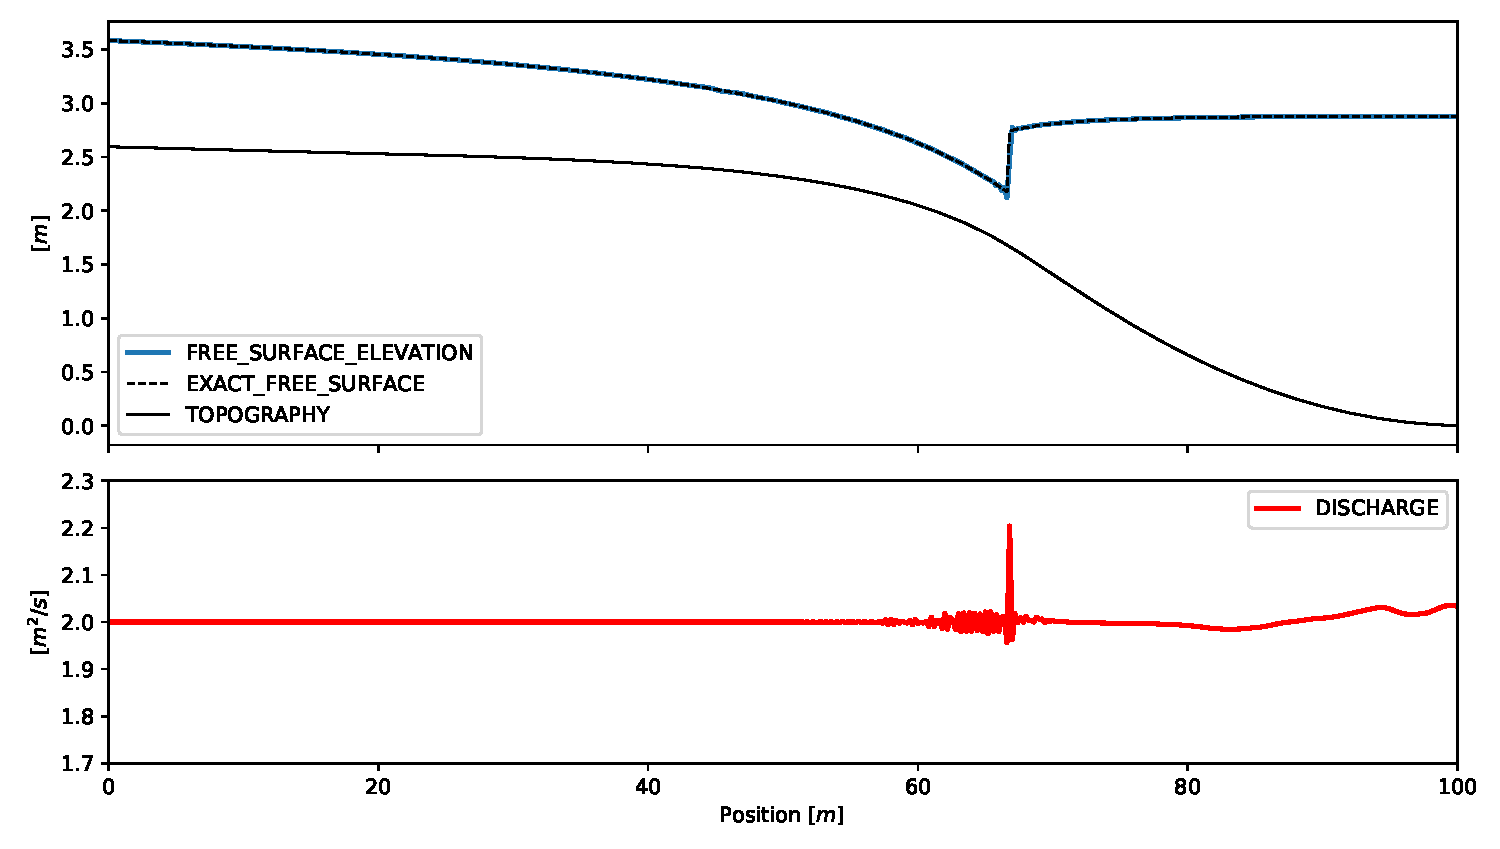
\includegraphics[width=\textwidth]{img/eulerian/jump/mesh_0.2.pdf}
        \label{mac_donald_shock_graph_2}
    \end{subfigure}
    \vspace*{-2em}
    \caption{Short channel. Graph along the cut defined by the center of the channel.}
\end{figure}


\subsection{Experimental dam break flow against an isolated building}
\label{sec:examples:experiment}


The last example consists on the reproduction of the experiment carried out by Soares \cite{soares2007}.
A dam break flow with a building downstream is simulated. The problem definition is depicted in Figure \ref{experiment_sketch}. The channel is $3.4m$ wide and the end of the dam is located at $x=0$.
As initial conditions, the water depth is set to $0.4m$ in the reservoir, while the channel is dry. The Manning coefficient is $0.01sm^{-\sfrac{1}{3}}$ over all the domain.
At the beginning of the simulation, the gate of the dam is removed and the water is allowed to flow around the building.

There are some gauges (Table \ref{gauges_positions} and Figure \ref{experiment_sketch}) where the water height and velocity are recorded. Experimental data is used to validate the numerical method.

\begin{figure}[H]
\centering
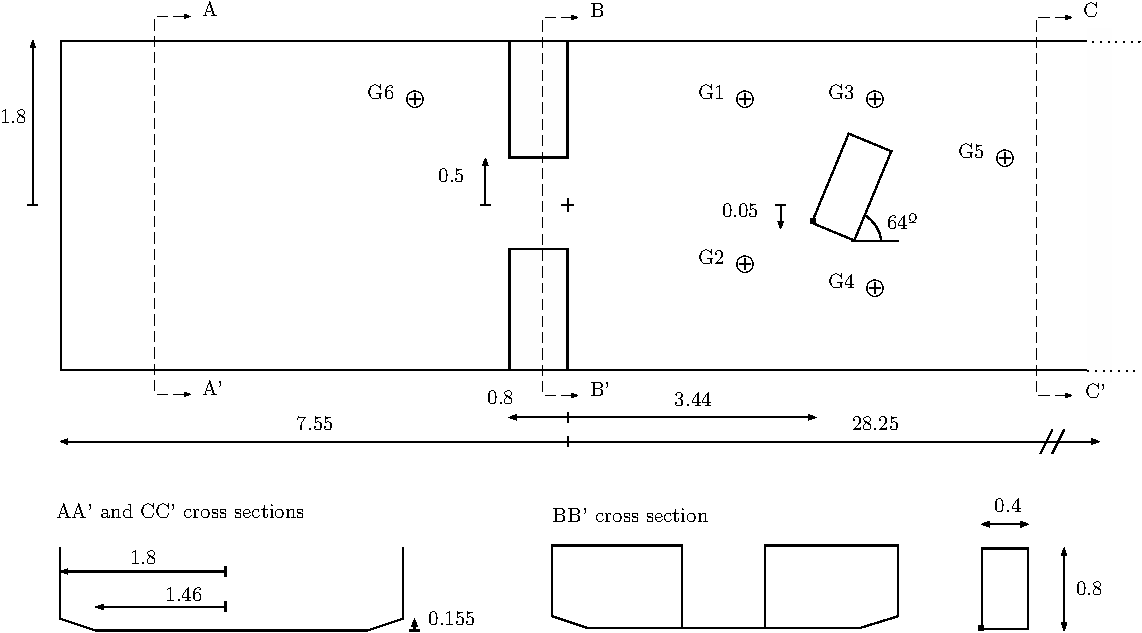
\includegraphics[width=\textwidth]{img/eulerian/exp/sketch.pdf}
\caption{Experimental dam break flow. Definition of the isolated building benchmark. The dimensions are in $m$.}
\label{experiment_sketch}
\end{figure}

\begin{table}
\centering
\begin{tabular}{ccc}
\hline
Gauge number & X & Y \\ \hline
1 &  2.65 &  1.15 \\
2 &  2.65 & -0.60 \\
3 &  4.00 &  1.15 \\
4 &  4.00 & -0.80 \\
5 &  5.20 &  0.30 \\
6 & -1.87 &  1.10 \\ \hline
\end{tabular}
\caption{Experimental dam break flow. Positions of the gauges, units in $m$.}
\label{gauges_positions}
\end{table}

The domain is discretized with a mesh with an average element size of $0.05m$. There are 115.000 elements and the time step is computed to keep a courant number of 1.0. Figure \ref{experiment_mesh} displays two details of the mesh, near the dam and around the building.

\begin{figure}[H]
\centering
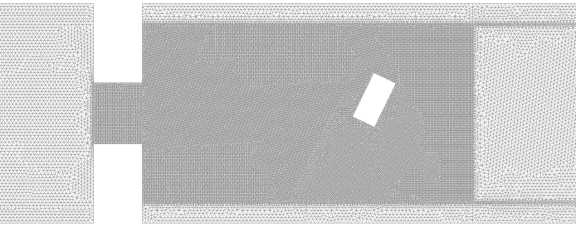
\includegraphics[width=.8\textwidth]{img/eulerian/exp/experiment_mesh.png}
\caption{Experimental dam break flow. Detail of the mesh near the dam and around the building. The coarse elements have an average size of $0.06m$ and the refined area has an average element size of $0.02m$. There are 160.000 elements.}
\label{experiment_mesh}
\end{figure}

To get a general idea of the flow, Figure \ref{experiment_plots} shows several results of the water depth after the gate release. Figure \ref{experiment_gauges} shows the evolution of the water depth at the gauges. An initial delay is observed in the propagation of the front in the gauges 1 to 5.

\begin{figure}
\centering
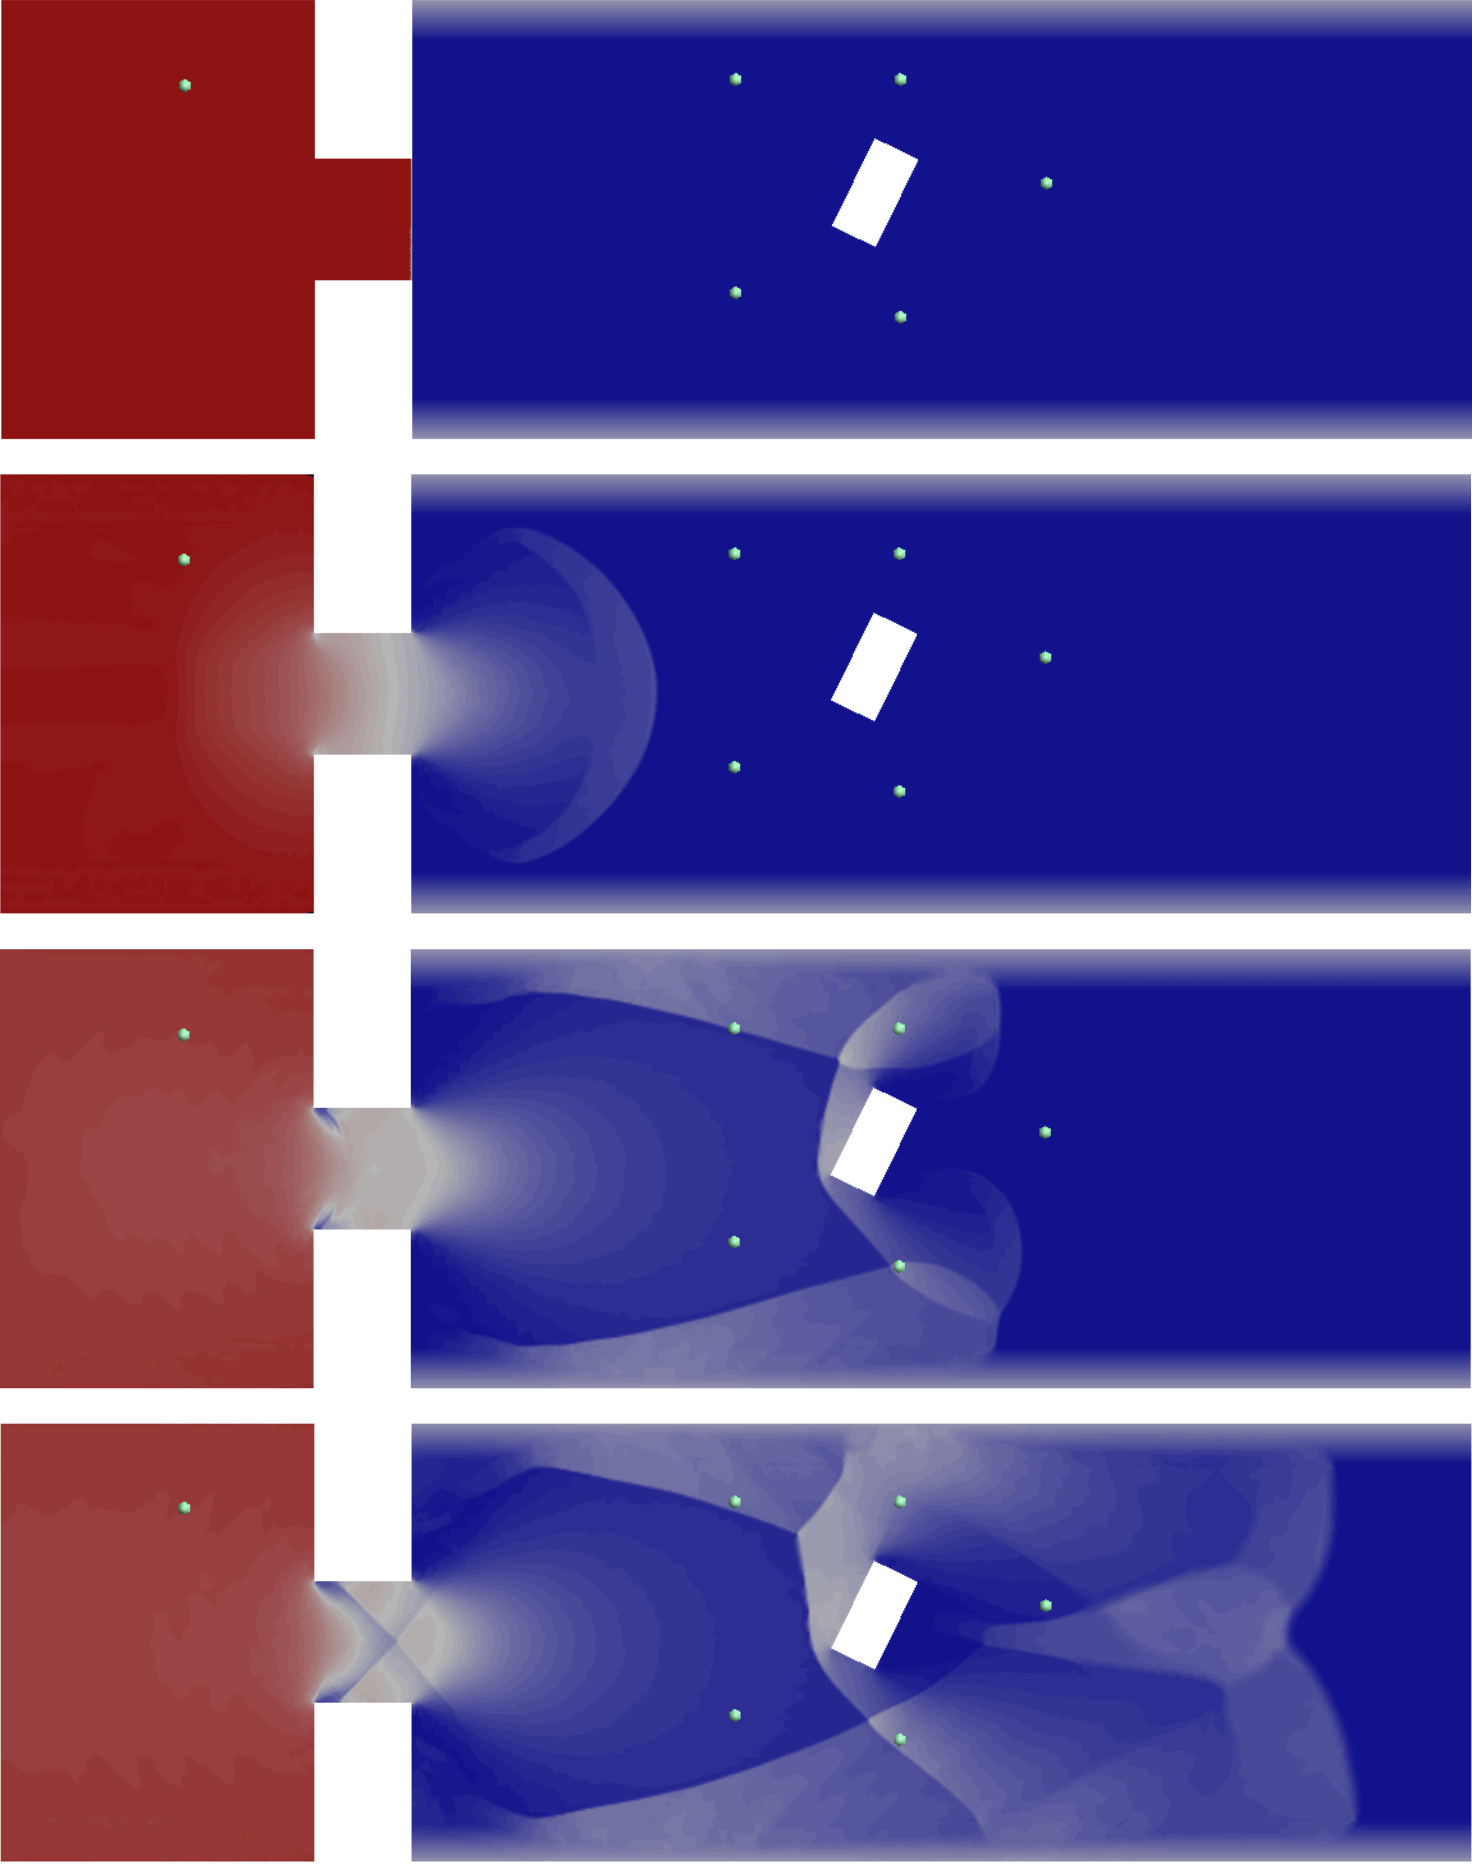
\includegraphics[width=\textwidth]{img/eulerian/exp/results.png}
\caption{Experimental dam break flow. Results of the benchmark at times $0$, $1$ and $3$ seconds}
\label{experiment_plots}
\end{figure}


Gauge 1 is located upstream of the building and close to the left wall of the channel. In gauge 1 there are the main discrepancies between the numerical and experimental results. The vicinity of the wall is responsible for the rapid variations in the water level. After the arrival of the front wave, this is reflected in the wall and a second raise of the water level is observed. About $t=6s$, an oblique hydraulic jump is formed and registered in gauge 1. The two first shocks are well captured by the numerical results, but the oblique hydraulic jump is registered latter, at $t=10s$, and there is a general overestimation of the ones for the water depth values.

The main hydraulic jump in gauge 2 formed by the reflection against the building is registered at $t=15s$, but in the numerical simulation is it formed very rapidly, presenting a discontinuity in time.

\begin{figure}
\centering
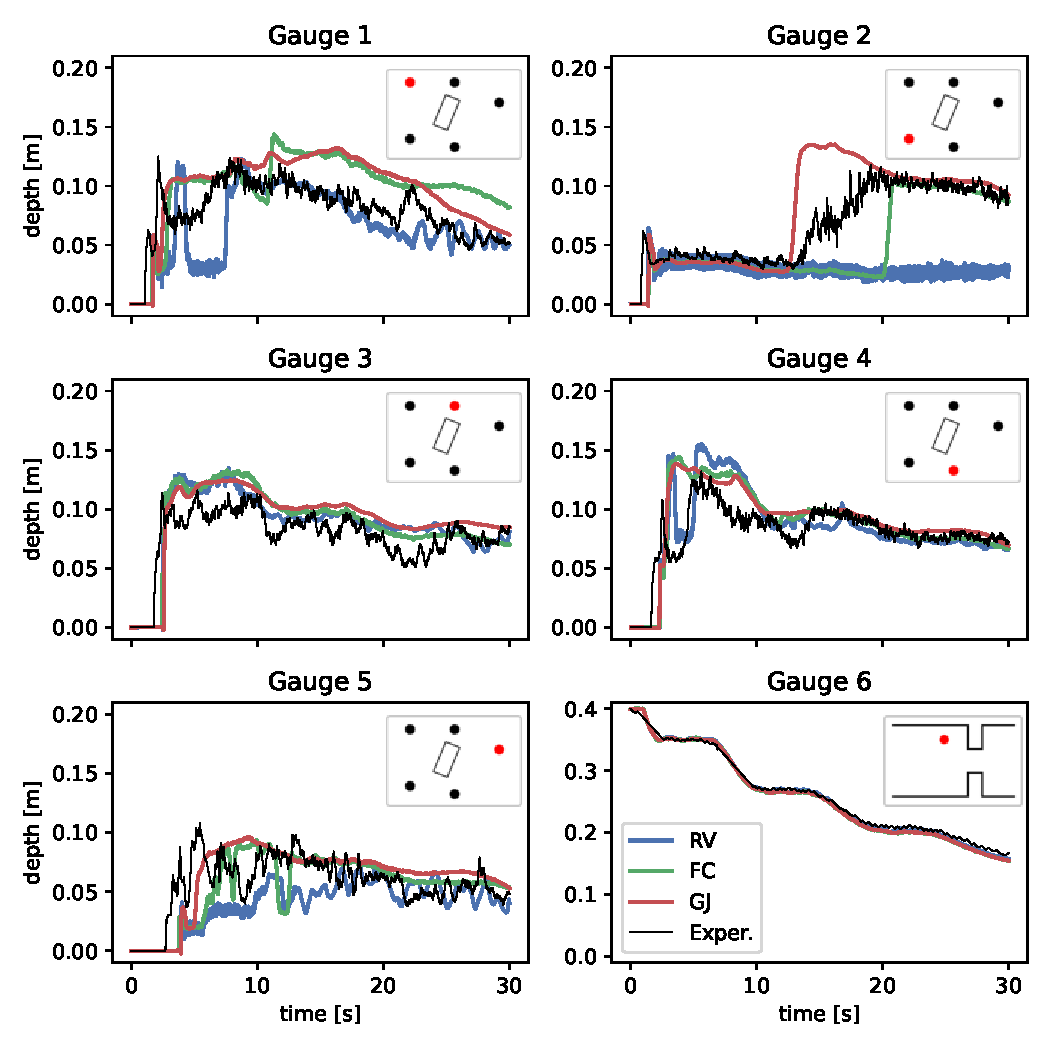
\includegraphics[width=\textwidth]{img/eulerian/exp/gauges.pdf}
\caption{Experimental dam break flow. Comparison between the obtained water depth with the reference data.}
\label{experiment_gauges}
\end{figure}

Gauge 3 is located at the left hand side of the building, where multiple waves are reflected and practically always it is in subcritical regime. There is a good correlation between numerical and experimental results. Gauge 4 is at the opposite side of the building but the superposition of the reflected waves is more clearly identified. The main discrepancies in the results are concentrated in the first seconds, where the flow is more dynamic.

Gauge 6 is located at the reservoir and registers the superposition of smooth waves during the emptying of the tank.

As stated in \cite{soares2007} there are some difficulties in the recording of the velocity and its validity is discussed. Here we compare only the most representative gauges. Gauge 2 is not fully submerged and the validity of the measurements is good after $t=14.5s$. It illustrates the change from supercritical flow to subcritical (Figure \ref{experiment_gauge2_vel}). The considerations are similar to the water depth study.


\begin{figure}
\centering
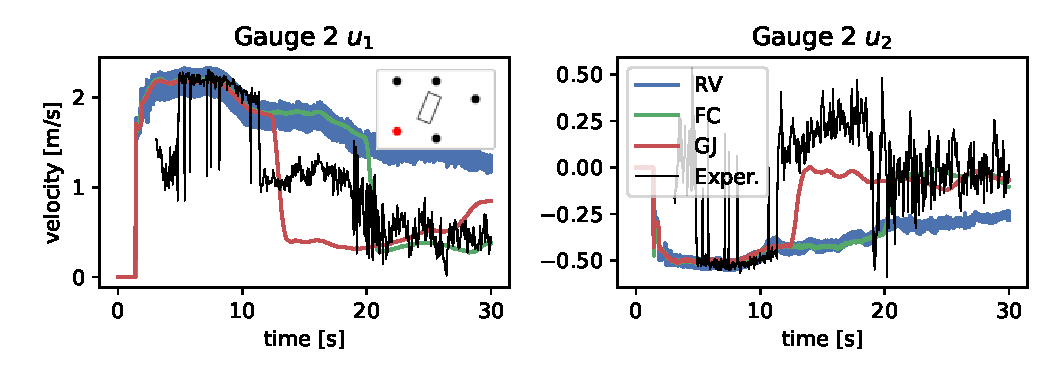
\includegraphics[width=\textwidth]{img/eulerian/exp/gauge2_vel.pdf}
\caption{Experimental dam break flow. Comparison of velocity at gauge 2.}
\label{experiment_gauge2_vel}
\end{figure}

The experimental measurements in gauge 4 (Figure \ref{experiment_gauge4_vel}) show a change in the velocity direction around $t=15s$ due to the rise of water level. The numerical results do not capture this change but the mean and the stationary values are correctly simulated.

\begin{figure}
\centering
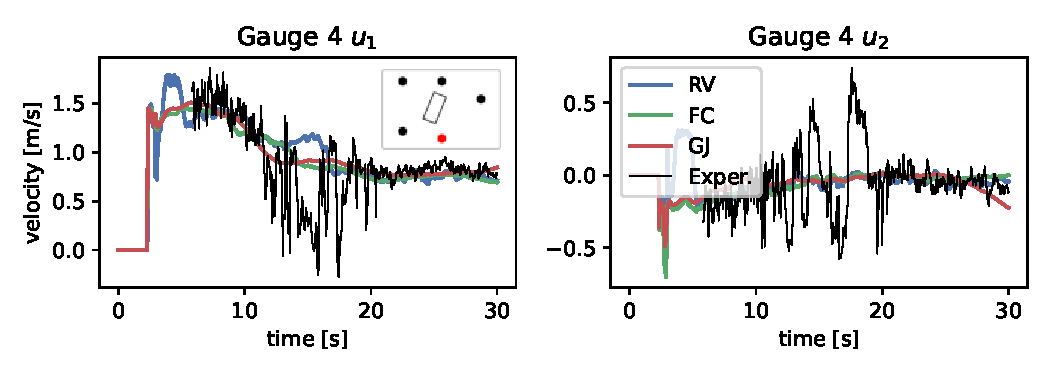
\includegraphics[width=\textwidth]{img/eulerian/exp/gauge4_vel.pdf}
\caption{Experimental dam break flow. Comparison of velocity at gauge 4.}
\label{experiment_gauge4_vel}
\end{figure}

In gauge 5 the formation of eddies behind the building can be appreciated from $t=20$ (Figure \ref{experiment_gauge5_vel}). In that case, the experimental results have difficulties to capture the eddies. Results will probably improve by extending the refined region of the mesh. The only method able to reproduce the eddies is the RV.


\begin{figure}
\centering
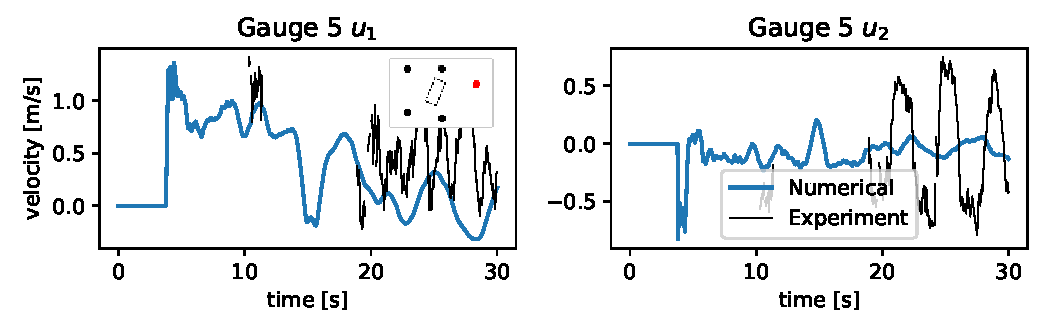
\includegraphics[width=\textwidth]{img/eulerian/exp/gauge5_vel.pdf}
\caption{Experimental dam break flow. Comparison of velocity at gauge 5.}
\label{experiment_gauge5_vel}
\end{figure}


In fluid-structure interaction studies, pressure is needed to compute to forces over the structure. The shallow water assumptions drop the dynamic pressures retaining only the hydrostatic ones. In the present case, the pressures are recovered by integrating the hydrostatic pressures given the water depth around the building. However, there is no experimental data about the forces applied to the building and thus, the importance of the dynamic pressures can not be evaluated.


Regarding the performance of the FIC-FEM formulation, it captures the main aspects of the flow, but not the details, since there are some regions on that experiment which violate the shallow water approximations.








\section{Concluding remarks}


In this chapter the Finite Element approximation for the shallow water equations has been presented. The interpolation of the solution to the shallow water equations using Finite Elements induces some difficulties which have been addressed.

The first problem is the instabilities related to the \emph{inf-sup} condition when the same interpolation is used for all the unknowns. The FIC-FEM formulation has been extended to the SW equations to overcome these instabilities. The main contribution is the projection of the characteristic length onto the linearization matrices $\mathbf{A}_i$. This procedure present an algorithmic constant and has been fixed to $\beta=0.01$.

The second and third issues are closely related. One is the rise of local instabilities around hydraulic jumps and the last is the Gibbs oscillations at the shoreline. Both phenomena are solved introducing enough diffusion near the problematic regions, this procedure is known as non-linear stabilization. Some traditional methods aiming to provide local stability have been extended to the SW equations.

The \emph{Residual Viscosity} (RV) method is firstly presented. It is the most consistent method among the three non-linear stabilizations presented in this chapter. Since the added viscosity depends on the residual, it introduces a non linearity and the order of convergence is lost in the regions where the non-linear stabilization is acting. Nevertheless, the global order of convergence is kept and good solutions are obtained. An algorithmic constant controls the amount of artificial viscosity introduced and it has been fixed to $\alpha=1.0$.

The second non-linear stabilization presented in this chapter is the \emph{Flux Corrected} (FC) algorithm, which combines two solutions. It could be used without linear stabilization, however, it is helpful to use a stabilized high order solution. Otherwise, phenomena such as terracing or excessive diffusivity, may appear.
There are some difficulties with the definition of the convergence criterion. Even if the incremental displacements of the iterative solution are used as a measure of the convergence, the desired convergence is slowly achieved. The required number of iterations is higher than those required for a RV shock capturing. A practical option is to limit the iterations up to a fixed number. However, this approach will lack an accurate control of the obtained precision for transient problems. For example, the flow in front an obstacle is highly dynamic and it might require more iterations than the prefixed number.

Furthermore, the extension of the FC principles to the SW equations is not monotonicity preserving. Apart from the linear stabilization, the main responsible of the lack of monotonicity is the flux limiter. The flux limiters were initially designed for pure convection problems and when those are extended to the SW equations some limitations arise. Mainly, there is no a unique decomposition in pure convection problems. Then, the naive option has been chosen in this chapter: to choose the water depth a indicator. This option lose the monotonicity but the solution is reasonably good without increasing the computational cost.

The computational cost of FC is high. Though the algorithm has to solve a system with the same number of degrees of freedom than a linear stabilized problem (\ref{sec:fic_fem_stabilization}), the introduction of the corrections is non linear. 
Regarding the global solution and its robustness, good results are obtained. However, a better order of convergence is expected.

Finally, the \emph{Gradient Jump Viscosity} (GJV) belongs to the same family than RV, since it it based on the introduction of viscosity. Though the extension of this method to more than one dimension is not monotonic, that is the less oscillatory method presented in this chapter. Its main drawbacks are the amount of additional viscosity and its lack of consistency with the source terms. Over-diffusive results have been observed in the last example, the dam break against an isolated building \ref{sec:examples:experiment}. Especially, the added diffusion inhibits the formation of shedding vortices behind the building. The lack of consistency is observed on the way the viscosity is added. Since the viscosity is not based on the residual but on the gradient jump, the presence of a high gradient on the topography will be translated on a region of additional diffusivity, even if the solution does not present a discontinuity.

To summarize, all the three methods have presented good results. There are slightly differences depending on the problem, if it is transient or stationary, if it presents a moving shoreline, if there are high topography gradients, etc. The preferred option is the RV method since it is consistent with the equations and it is derived from the linear stabilization. This method will be used in the following chapters.



\chapter{Finite Element Method for the Boussinesq modified equations}
\label{eulerian_bsq}


In this chapter, a FEM approximation for the Boussinesq modified equations is presented. Having a numerical approximation for the Boussinesq modified equations is mandatory when waves are studied on a two dimensional scenario and a complex bathymetry is considered.

\textcolor{red}{Some comments about numerical methods, a short state of the art.}

Several numerical models appeared in the bibliography to solve the Boussinesq equations, under the possible variations for considering the dispersive terms. Abbot pioneered the FD schemes in \cite{abbott1978,abbott1979} applied to the original Boussinesq model. Later, Wei and Kirby solved the modified equations presented by Nwogu \cite{nwogu1993} using a FD scheme in \cite{wei1995}. The main advantage of the FD is the ease of treatment higher differences, even though the main difficulty consists on representing complex domains. Smallman was a pioneer applying the FD to harbours \cite{smallman1989}.

A decade later, some FEM were developed to solve Boussinesq equations. In that case, some special treatment needs to be applied to the high order derivatives. Langtangen \cite{langtangen1998} used quadratic triangles while most of the authors use aan intermediate variable. Li and Liu \cite{li1999} used bilinear quadrilaterals and used a projection to approximate the gradient. Walkley \cite{walkley2002} and Woo \cite{woo2004a,woo2004b} used a projection to interpolate the second order derivatives filed. Surprisingly, the authors reported high frequency oscillations and proposed ad-hoc solutions, but until Codina \cite{codina2008,codina2008b} none of them associated the oscillations to the incompatibility of interpolation.

The method has been solved using DG \cite{eskilsson2002} and FV \cite{bradford2002,stansby2003}. As reported by Stansby \cite{stansby2003}, since the FV is non-oscillatory, needs special techniques to accurately approximate the oscillatory behavior of the Boussinesq equations.

This chapter includes the developments presented in chapter \ref{eulerian_sw} and adds the new techniques associated to the oscillatory and dispersive problem. 
Som examples are included in order to test the accuracy and to show the capabilities of the presented algorithms.
Finally, the chapter is closed with the concluding remarks.



\section{Stabilized formulation for the Boussinesq modified equations}



As stated in section \ref{equations}, the Boussinesq equations and the Saint Venant equations are of the same family. Apart from the choice of different primary variables, the main difference consists on the inclusion of the dispersive terms. However, part of the structure of the equations remains unmodified.

The weak principle, the linear stabilization and the spatial discretization presented in section \ref{eulerian_sw} will be directly applied for the Boussinesq modified equations. The main differences arise from the dispersion terms.
First of all, the dispersion terms include spatial derivatives of order higher than two. Thus, special techniques for considering the third order derivatives will be included in the FEM procedure.

Secondly, the time discretization will be modified using a semi-implicit fourth-order scheme. The new time scheme allows to deal with the oscillatory behavior of the Boussinesq equations.
Additionally, the matrix structure will suffer some modifications related to the high order derivatives and the time integration scheme.

Regarding the shock capturing, usually it is not needed since the dispersion effect prevents from breaking and the formation of steep gradients. However, in the vicinity of the shoreline or very shallow domains, the amplitude dispersion effect could dominate over the frequency dispersion, making very recommended the inclusion of a shock capturing technique. Furthermore, if the shoreline is included, the shock capturing is required, since it provides stabilization for the moving front.

On another note, a section regarding the numerical treatment of absorbing boundary conditions is included. The inclusion of the frequency dispersion and the need of shortening the computational domain, lead to the open boundary conditions. On an open boundary conditions, waves can exit the computational domain and reflections must be avoided. The numerical approximation for the open boundary conditions are called absorbing boundary conditions.



%%%%%%%%%%%

The Boussinesq modified equations need to be stabilized. In this section the linear stabilization presented in \ref{sec:fic_fem_stabilization} will be applied. Since the Boussinesq equations are intended to solve oscillatory problems, the shock capturing is not relevant. However, an additional technique must be introduced in order to deal with the higher order derivatives.

In this section, the boundary conditions considered by the numerical model will be introduced. Then, the numerical procedure is explained. Here, the introduction of a gradient recovery is presented. After presenting the formulation for solving the equations, a numerical procedure for the absorbing boundary conditions will be proposed. Finally, some examples are added.





\subsection{Weak formulation and spatial discretization}


The Boussinesq equations are solved using the FEM. The space domain is interpolated with a Galerkin discretization of linear triangles and a finite difference scheme with constant time step is used to integrate the equations in time.
Some numerical difficulties such as the third order differential operator and the time integration accuracy are addressed in \cite{walkley2002,woo2004a,wei1995}.
As stated by Codina in \cite{codina2008,codina2008b} the problem (\ref{bsq_eq}) is an hyperbolic wave in mixed form and there is an incompatibility condition (see \cite{BrezziFortin}) because the same interpolation is used for both variables, the velocity $\mathbf{u}_\beta$ and the wave amplitude $\eta$.
Here the equations are stabilized using FIC extending the work done in \cite{maso2022}.


\subsection{Derivatives recovery}

Following \cite{walkley2002}, the third order spatial derivatives are modelled using $\mathbf{J}_\eta$ as an intermediate variable. There are several ways of computing the intermediate field $\mathbf{J}_\eta$. The first possibility is to compute it in a monolithic way, adding $\mathbf{J}_\eta$ to the degrees of freedom.

A more interesting option is to compute it in a staggered way using a projection. In that case, the number of degrees of freedom is not increased and thus the time consuming performance of the scheme is unaltered. 

finally, the projection for the auxiliary field $\mathbf{J}_\eta$ can be replaced by a gradient recovery technique. In that section this option is analyzed, since the gradient recovery provides more regularity, at the same time, it is very efficient.

The gradient recovery technique was initially proposed by Zienkiewicz and Zhu in \cite{zienkiewicz1992}. Later, Zhang and Naga proposed some improvements for the super convergent gradient recovery in \cite{zhang2005} at boundaries. Finally, some improvements have been proposed in \cite{wu2007,ahmed2021} for adaptive meshes, but the last improvements are not going to be considered in this research. The basis of the gradient recovery consists on fitting a $k+1$ polynomial degree where the finite elements space is of degree $k$.

The main idea of the gradient recovery is to introduce an operator $G_h : S_h \rightarrow S_h^{n_d}$, where $S_h$ is a polynomial finite element space of degree $k$ over a triangulation $T_h$ and $n_d$ is the space dimension. After determining the values of $G_h$ at all nodes, given a solution $u_h$ , $G_h u_h \in \S_h^{n_d}$ is obtained on the whole domain.
The triangulation can be replaced by a quadrilateral discretization. In both cases, only vertices nodes are considered, nor edge or internal nodes.

For a vertex $\mathbf{x}_i$ and being $l_i^e$ the size of the largest edge attached to $\mathbf{x}_i$, a ball is defined around it:
\begin{equation}
    B_{l_i^e}(\mathbf{x}_i) = \{ \mathbf{x} \in T_h : \vert \mathbf{x} - \mathbf{x}_i \vert \leq l_i^e \}
\end{equation}
and all the vertices inside the ball are selected. If the number of nodes $n_n$ inside the ball $B_{l_i^e}(\mathbf{x}_i)$ is less than $m = (k+n_d) (k+n_d+1) / 2$, then the ball is extended to two times the edge length, $B_{2l_i^e}$. This process of increasing the radius is repeated until there are enough nodes in the ball. The nodes inside a ball are denoted as $\mathbf{x}_{ij}$ and the polynomial $p_{k+1}$ is fitted using local coordinates with $\mathbf{x}_i$ at the origin and the scaling parameter $l=l_i^e$,
\begin{equation}
    p_{k+1} = \mathbf{P}^T \mathbf{a} = \hat{\mathbf{P}}^T \hat{\mathbf{a}}
\end{equation}
where
\begin{subequations}
\begin{equation*}
         \mathbf{P}^T  = (1,x,y,x^2,...,x^{k+1},x^ky,...,y^{k+1}), \quad
    \hat{\mathbf{P}}^T = (1,\xi,\eta,\xi^2,...,\xi^{k+1},\xi^k\eta,...,\eta^{k+1})
\end{equation*}
\begin{equation*}
         \mathbf{a}^T  = (a_1,a_2,...,a_m), \quad
    \hat{\mathbf{a}}^T = (a_1,la_2,...,l^{k+1}a_m),
\end{equation*}
\end{subequations}
And the coefficient vector $\mathbf{a}$ is determined by the linear system
\begin{equation} \label{superconvergent_polynomial}
    A^T A \hat{\mathbf{a}} = A^T \mathbf{b}_h
\end{equation}
where $\mathbf{b}_h^T = (u_h(\mathbf{x}_{i1}), u_h(\mathbf{x}_{i2}), ... , u_h(\mathbf{x}_{in_n}))$ and
\begin{equation*}
A = \left(\begin{matrix}
    1 & \xi_1 & \eta_1 & ... & \eta_1^{k+1} \\
    1 & \xi_2 & \eta_2 & ... & \eta_2^{k+1} \\
    \vdots & \vdots & \vdots & \ddots & \vdots \\
    1 & \xi_{n_n} & \eta_{n_n} & ... & \eta_{n_n}^{k+1} \\
\end{matrix}\right)
\end{equation*}
A condition for (\ref{superconvergent_polynomial}) having solution is that $Rank(A) = m$, which is practically always satisfied when $n_n > m$ and the mesh has a reasonable quality. Finally, it is possible to define the gradient at the point $\mathbf{x}_i$ as
\begin{equation}
    G_h u_h (\mathbf{x}_i) = \nabla p_{k+1} (0,0,\mathbf{x}_i)
\end{equation}

Similarly, the gradient of a divergence can be obtained when the polynomial is applied to a vector field. This procedure can be applied up to derivatives of order $k+1$, which for linear elements are second-order derivatives. Finally, the gradient of the divergence reads
\begin{equation}
    L_h u_h (\mathbf{x}_i) = \nabla \nabla \cdot p_{k+1} (0,0,\mathbf{x}_i)
\end{equation}

Since the values of the nodal unknowns $u_h$ are not known a priory, the vector of coefficients $\mathbf{a}$ will be expressed as a linear combination of $u_h(\mathbf{x}_{ij})$. Depending on which derivatives of $\mathbf{P}$ are seek, the linear combination will be some selected rows of $(A^T A)^{-1}A^T$.




\subsection{Time discretization}

Finally, the problem (\ref{bsq_eq}) is expressed in matrix form as
\begin{equation} \label{sw_system_matrix}
    (M + K) \dot{x} = F(x,y)
\end{equation} 
where $x$ is the vector of nodal unknowns, $y$ is the vector of nodal values corresponding to $\mathbf{J}_\eta$, $M$ is a mass matrix, $K$ correspond to the second derivatives associated to $\mathbf{J}_{\mathbf{u}}$, and $F$ is a non-linear vector which is a function of $\mathbf{u}_\beta$ and its spatial derivatives.



The commonly used fourth order Adams-Moulton scheme is employed for the time integration of (\ref{sw_system_matrix}), see \cite{wei1995,woo2004a,codina2008b} as an example.
To obtain a solution at the time step $t^{n+1}$, the fixed point iterative method is employed to deal with the non-linearity of the system. Given a guess $x^{n+1,i-1}$ for $x^{n+1,i}$ at iteration $i$, the increment $\delta x^i$ is computed from
\begin{multline}
    24 (M + K) \delta x^i = 
    24 (M + K) (x^n - x^{n+1,i-1}) \\
     + \delta t (9F^{n+1} + 19F^n - 5F^{n-1} + F^{n-2}) + O(\delta t^4)
    \label{adams-moulton}
\end{multline}
The time integration is closed using the explicit third order Adams-Bashforth scheme to predict the initial guess $x^{n+1,0}$ for the non-linear iterations
\begin{multline}
    12 (M + K) x^{n+1,0} = 
    12 (M + K) x^n \\
     + \delta t (23F^n - 16F^{n-1} + 5F^{n-2}) + O(\delta t^3)
    \label{adams-bashforth}
\end{multline}

The system of (\ref{adams-moulton}) and (\ref{adams-bashforth}) is solved using a direct solver. Given the problem is small, this is not expensive.
Convergence is achieved when $\delta x^i$ is sufficiently small. Then, the solution $x^{n+1}$ is set as $x^{n+1,i}$.





\subsection{Absorbing boundary conditions}
\label{eulerian_bsq_absorbing}


Frequently, the need to shorten the numerical domain arises. This can be achieved by the imposition of open boundaries, also known as radiant boundaries. The open boundaries allow the exit of the waves as well as the consistency of the system of equations in order to ensure the existence and uniqueness of the solution. Additionally, the numerical tool for the boundary has to be compatible with the numerical approach for the inner domain.

Generally, the radiant boundary condition denotes the analytical formulation for open boundaries and the term absorbing boundary is related to the numerical approximation of the radiation condition \cite{navon2004}. An equilibrium between the precision offered by the radiant boundary and the numerical cost required by the absorbing boundary is seek.
From one side, the boundary conditions must define a well posed problem and the spurious oscillations in the open boundary shall be as small as possible. From the other side, the computational cost of the boundary conditions should be small compared to the computational cost of the inner domain.

Considering the unidirectional wave propagation and being $\eta$ the free surface elevation, a wave function will verify a radiant boundary condition where
\begin{equation} \label{radiation_condition}
    \pder{\eta}{t} + c \cos(\theta)\pder{\eta}{x} = 0
\end{equation}
where $\theta$ is tha incidence angle of the wave with respect to the boundary.

Some authors proposed local approximations highly diffusives \cite{engquist1977}. Latter, Bayliss explored the radiation boundary conditions for the Helmholtz equations in \cite{bayliss1982}.
Similarly, Collino \cite{collino1993} extended the formulation using higher order of derivatives than \ref{radiation_condition}. However, the generalization for the Euler equations -analogously the SW equations- in 2 or 3D is not trivial, since the incidence angle $\theta$ is not known \emph{a priori} and because of the dispersive behavior of the equations \cite{wei1995}.

The dispersive behavior is associated to the fact that there is not an unique celerity characterizing the system: in the case of the SW or the Boussinesq equations there are three waves superposed propagating at different speeds. For example, in section \ref{sec:sw_fc} a decomposition in characteristics was presented through diagonalization of the tangent matrices $\mathbf{A}_i$.
\begin{equation}
    \pder{\bm\Phi_j}{t} + \bm\Lambda_i \pder{\bm\Phi_j}{x_i} = 0
\end{equation}
in that minimal wave equation $\bm\Lambda$ is a diagonal matrix such that $\bm A_i = \bm T_i \bm\Lambda_i \bm T_i^{-1}$.
This problem can be understood a the superposition of three waves, each one of them propagating at speed $u-c$, $u$ y $u+c$, namely the eigenvalues $\lambda_i$. The sign of $\lambda_i$ determines if the wave is incoming or outgoing and the regime of the problem: subcritical or supercritical.

Besides having to impose the radiant boundary condition for the three waves, this approximation is limited, since in 2 or 3D does not exist a genuine characteristic-based formulation. A more detailed development can be found in \cite{lie2001}.

Most of the proposals to approximate the open boundaries consist on relaxing the condition \ref{radiation_condition}  adding a dissipation term $K$ and extending the domain a distance $d$, losing the local definition. See \cite{israeli1981,navon2004,carmigniani2018} as an example. Then, the radiation condition is rewritten as
\begin{equation} \label{radiation_absorbing_condition}
    \pder{\eta}{t} + c \cos(\theta)\pder{\eta}{x} = -K\eta
\end{equation}
This approximation can be used in combination with local absorbing boundary conditions \cite{wei1995}.

Another of the explored possibilities is the Perfectly Matched Layer (PML) \cite{berenger1994}, widely used in the literature. It presents the inconvenient of special treatment of corners.
Later, this methodology wa used in combination with the high order absorbing boundaries, leading to the Double Absorbing Boundary (DAB), proposed by Hagstrom and Rabinovich in \cite{hagstrom2014,rabinovich2015}. This technology places two parallel boundaries separated by a short distance. Its advantage is that they do not need to incorporate the derivatives in the normal direction neither to apply any special treatment to the corners.

Finally, and given to the simplicity of the formulation, there is the possibility of including only a sponge layer. It can be found in the formulations of Israeli and Carmigniani in \cite{israeli1981,carmigniani2018}. A Newtonian dissipative term analogous to the bottom friction $S_f$ is added as
\begin{equation}
    S_a = -\gamma(\mathbf{x}) \mathbf{u}
\end{equation}
The dissipative term $\gamma$ varies from 0 at a given distance to the discrete boundary to the maximum value $\gamma_{max}$ at the discrete boundary. This variation follows an exponential law \cite{peric2018} of order $n$. The parameters of the sponge layer $d_0$ and the maximum value $\gamma_{max}$ need to be specified for each case, in terms of the wavelength.
A possible expression for $\gamma$ is
\begin{equation} \label{exponential_sponge_layer}
    \gamma(\mathbf{x}) = \gamma_{\max} \mathcal{H}(d_0 - d(\mathbf{x})) \frac{e^{\left(\frac{d_0 - d(\mathbf{x})}{d_0}\right)^n} - 1}{e - 1}
\end{equation}
where $\mathcal{H}$ is the Heaviside function, $d$ is the distance from a point to the computational boundary.

In Fig. \ref{absorbing_boundary} the propagation of a train of regular waves is shown. Ate the left end of the domain, waves are generated. At the right end of the domain there is a sponge layer. Studies carried out by Carmigniani in \cite{carmigniani2018} show that some combinations of the maximum absorption, layer width and exponential degree can produce undesired reflections. For example, an excessive absorption can generate reflections at the beginning of the sponge layer.

An exponent $n=3$ for expression \ref{exponential_sponge_layer} is chosen, it considerably minimizes the reflection \cite{carmigniani2018}. A sensibility analysis of the parameters $d_0$ y $\gamma_{\max}$ should be done.
It is useful to express the maximum distance and absorption in terms of the wavelength and frequency. In practice, the width of the sponge layer is used to be $d_0 \approx 2\lambda$ and the absorption coefficient $\gamma \approx 0.5\omega$.

The reflected amplitude is monotonically decreasing as the sponge width increases. Nevertheless, the reflection exhibits a local minimum with respect to the absorption coefficient. This makes highly recommended to adjust the parameters of the sponge layer according to the  maximum wavelength.


\begin{figure}
    \centering
    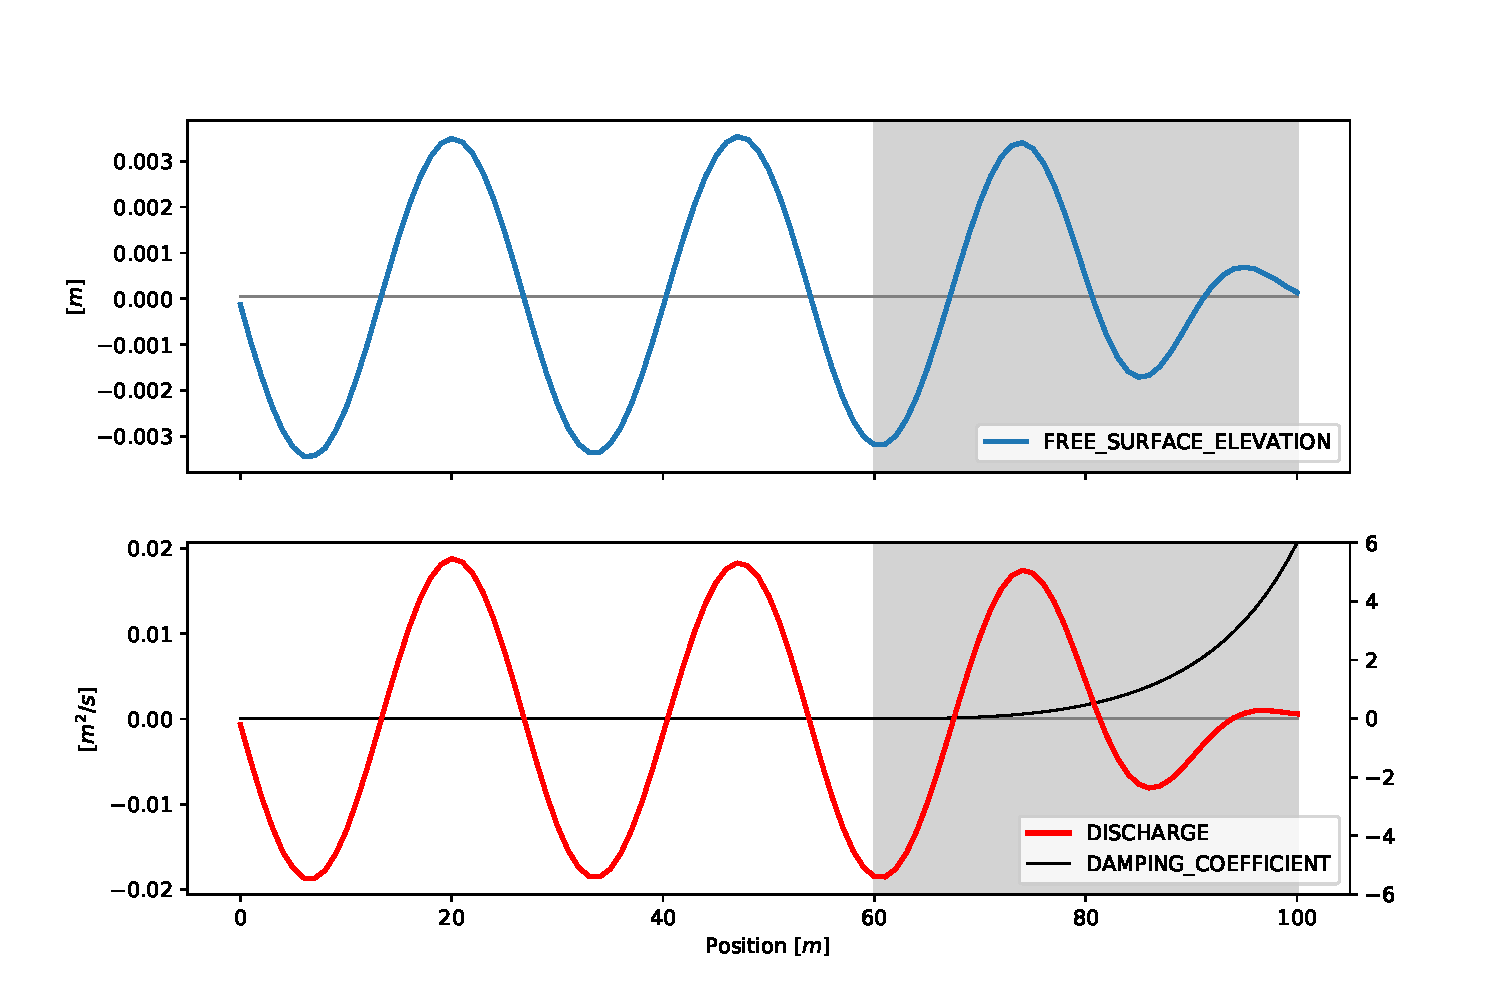
\includegraphics[width=.8\textwidth]{img/absorbing_boundary/absorbing_boundary.pdf}
    \caption{Propagation and absorption of a train of waves. The shadow region shows the width of the sponge layer.}
    \label{absorbing_boundary}
\end{figure}


\section{Examples}


\subsection{Solitary wave propagation}


\subsection{Absorbing boundary}



\section{Concluding remarks}




\chapter{Coupling strategies between reduced and fully resolved models}
\label{coupling}




\chapter{Conclusions}
\label{conclusions}



%%%%%%%%%%%%%%%%%%%%%%%%%%%%%%%%%%%%%%%%%%%%%%%%%%%%%%%%%%%%

\section{Achievements}




%%%%%%%%%%%%%%%%%%%%%%%%%%%%%%%%%%%%%%%%%%%%%%%%%%%%%%%%%%%%

\section{Further research}


\begin{enumerate}
    \item ALE for SW
    \item Optimizations of stability properties
    \item Coupling from SW to NS
    \item FSI problems
\end{enumerate}




%----------------------------------------------------------------------------------------
%	THESIS CONTENT - APPENDICES
%----------------------------------------------------------------------------------------

\appendix % Cue to tell LaTeX that the following "chapters" are Appendices


\chapter{Particle Finite Element Methods for the shallow water equations}
\label{lagrangian_sw}




In the previous chapter the SW equations have been analyzed considering the coupled convective and oscillatory mechanisms in an Eulerian framework. However, in some regions of the domain, the solution of the equations can be convection dominated. Specifically, where there is a movement of the shoreline --like run-up or flooding--, the problem is convection dominated.
This mechanism suggests the use of Lagrangian strategies, which have been successfully applied to convection diffusion and Navier-Stokes problems.

In this chapter, the developments of the Particle Finite Element Method (PFEM) are applied to the SW equations. The basis of the PFEM family of methods consists on a splitting operator, solving two stage fashion the convective operator and the rest of the equations. In the case of the SW equations, there is a stage for convection and other stage for wave mechanism.
The main advantage of the PFEM lies in using the variational principle of FEM. Hence, the formulations presented in chapter \ref{eulerian_sw} are applicable with small modifications. The novelty of the PFEM consists on solving the convection with a particle method.

In the family of PFEM there are two main groups, the moving mesh and the fixed mesh. The mesh moving algorithm was firstly presented to the scientific community \cite{idelsohn2003,idelsohn2004} and has been widely applied to a high number of situations \cite{larese2008,Salazar2012,onate2008}. In this method, the particles traditionally coincides with the nodes. After the convection stage --and eventually, remeshing--, the mesh inherits the displacements of the convection. Those displacements are part of the material derivative involved in the variational principle of the equations.

Lately, a second generation of the PFEM was presented \cite{idelsohn2012}. It uses a fixed mesh and is known as PFEM-2. The main idea consists on decoupling the particles from the nodes, leading to a duality of spaces: the FEM discretization and the particles discretization. Its main drawback is the introduction of projections between the two spaces but the cost of the projection is expected to be recovered by the use of a fixed mesh strategy without remeshing \cite{idelsohn2015,puigferrat2021}.



\section{Introduction}

The Lagrangian formulation starts by the definition of the material derivative. Let $\varphi$ be a scalar or vector property, the material derivative is obtained by applying the chain rule:
\begin{subequations} \label{mat_derivative}
\begin{align}
\frac{D}{Dt}\varphi(\mathbf{x},t) &= \pder{\varphi}{t} + u\cdot\nabla\varphi \label{mat_derivative:deriv} \\
\pder{\mathbf{x}}{t} &= \mathbf{u} \label{mat_derivative:conv}
\end{align}
\end{subequations}
The Lagrangian procedure consist on solving separately the equations (\ref{mat_derivative:deriv}) and (\ref{mat_derivative:conv}). To apply this staggered procedure, a generic conservation balance is considered,
\begin{equation} \label{conserv_balance}
\pder{\varphi}{t} + \nabla \mathbf{F} = 0
\end{equation}
where $\mathbf{F}$ is the fluxes vector in an infinitesimal volume of control. The balance equation is split into the convective and non convective fluxes, $\mathcal{L}_1$ and $\mathcal{L}_2$ respectively.
\begin{equation} \label{spatial_balance_linearized}
    \pder{\varphi}{t} + \mathcal{L}_1 \varphi + \mathcal{L}_2 \varphi = 0
\end{equation}
After introducing equation (\ref{mat_derivative}) into (\ref{spatial_balance_linearized}), the following expression is obtained,
\begin{equation} \label{mat_balance_liearized}
    \frac{D\varphi}{Dt} + \mathcal{L}_2 \varphi = 0
\end{equation}

Finally, the numerical strategy for solving a balance equation (\ref{conserv_balance}) in a Lagrangian framework consists on applying a splitting, generally, the first order Godunov splitting \cite{leveque2002} or the second order Strang splitting \cite{macnamara2016}.
The order of accuracy of the splitting operator is related to the sequence and the mode how equations (\ref{mat_derivative:conv}) and (\ref{mat_balance_liearized}) are temporally integrated.





\section{Mesh moving methods}


The PFEM method has been widely applied to solve the incompressible Navier-Stokes equations, especially with free surface problems \cite{larese2008}, multi-fluids \cite{mier2010} and fluid-structure interaction \cite{onate2008}.
The moving mesh allows to fit the sub-domains with the discretization and the boundaries are tracked in a natural way.
When the PFEM is applied to the SW equations, the mesh moving will be solving the water domain in the horizontal plane. That is, the moving shoreline in the SW equations is playing the role of the free surface in the NS equations.

Once the discretization describes and follows the fluid motion --$\eta$ and $\mathbf{u}$--, there appears the need to introduce another discretization to define the fixed topography and its variations --$z$--, since it does not move with the fluid. The duality of discretizations introduce the need of a mapping between the two meshes. The topography data need to be mapped to the computational mesh for solving the equations. And the primal variables need to be mapped to the topographical mesh for visualization purpose. See figure \ref{pfem_dual_mesh}, where the fluid domain $\Omega_w$ si inside the computational domain $\Omega$. The topographic domain $\Omega_T$ coincides with the computational domain $\Omega$.
This approach presents some analogies with embedded formulations, except on the fact that the discontinuity is on the fluid --computational domain-- instead of the topography --geometric domain--.


\begin{figure} [ht]
    \centering
    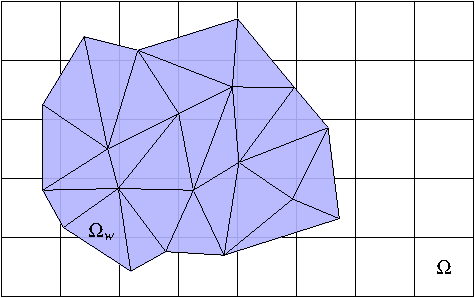
\includegraphics[width=.6\textwidth]{img/lagrangian/dual_pfem_mesh.pdf}
    \caption{Spatial discretization for the mesh moving PFEM algorithm.}
    \label{pfem_dual_mesh}
\end{figure}

Going back to the definition of the SW flow, the set of particles moving in the Lagrangian frame, convect the intrinsic properties (density, water depth, velocity, flow rate, etc.). The equations follow an \emph{updated lagrangian} formulation, that is, the variables are assumed to be known at time $t$ but unknown for the time $t+\Delta t$. Given that the variational principle is used to solve the equations in the continuum media, those is identified with the fluid domain, excluding the dry part. Once the convection is solved and the shoreline is updated, the system of equations is solved again.

Some modifications to this procedure may be considered. For example, an excessive deformation of the elements, without inverting them, may require a remeshing step. In that case, the identification of the shoreline coincides with the previous time step, but the interior domain will be refined. With a proper mesh quality control, the remeshing step can be applied only to those steps which really need it.

Additionally, an iterative scheme can be introduced, since the solution of the nwe system of equations at time step $t + \Delta t$ modifies the integration of the convective term. Usually this outer iteration loop is skipped by an explicit approximation of the convective term. The full path of the solution procedure is resumed in figure \ref{sw_pfem_algorithm}.

\begin{figure} [ht]
    \centering
    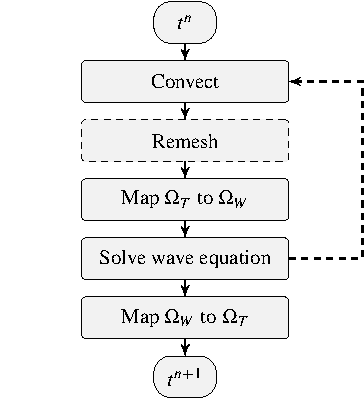
\includegraphics[width=.6\textwidth]{img/lagrangian/sw_pfem_algorithm.pdf}
    \caption{PFEM algorithm for the SW equations.}
    \label{sw_pfem_algorithm}
\end{figure}





\subsection{Governing equations}


Given that the nodes of the SW discretization are particles, the intrinsic properties are in a Lagrangian frame, thus, both mass and momentum balances follow a Lagrangian formulation. This fact reduces the non-linearity of the system of equations to be solved, making them easier to solve. On the other hand, in the Lagrangian framework the convection can be evaluated in terms of the primitive variables. We will take advantage of this characteristic to solve the primitive SW, which are more linear than the conservative ones.
The accuracy of the solutions obtained with the proposed method will be compared against the methods presented in the previous chapter.

Let the conservative vector of unknowns $\bm\phi$ be expressed in terms of the primitive set of variables $\bm\psi$. we recover the SW equations in terms of the primitive variables:
\begin{subequations}
\begin{align}
    \pder{\mathbf{u}}{t} &= \mathbf{u} \cdot \nabla \mathbf{u} + g \nabla(h-z_b) + g\mathbf{S}_f = \mathbf{0} \\
    \pder{h}{t} &= \mathbf{u} \cdot \nabla h + h \nabla \mathbf{u} = 0
\end{align}
\end{subequations}
The introduction of the material derivative definition yields
\begin{subequations} \label{pfem_mat_balance}
\begin{align}
    \frac{D\mathbf{u}}{Dt} &= g \nabla(h-z_b) + g\mathbf{S}_f = \mathbf{0} \\
    \frac{Dh}{Dt} &= h \nabla \mathbf{u} = 0
\end{align}
\end{subequations}

Analogously to the previous sections, if the solution $\psi$ is sufficiently smooth, it will also verify the quasi-linear form
\begin{equation} \label{pfem_mat_balance_lin}
    \frac{D\bm{\psi}}{Dt} + \mathbf{A}_i\pder{\bm{\psi}}{x_i} + \mathbf{S}\bm{\psi} + \mathbf{T} = 0
\end{equation}
Where the matrix $\mathbf{S}$ and the vector $\mathbf{T}$ are the same than those defined in section \ref{equations}. The tangent matrices $\mathbf{A}_i$ have a new expression for this case, according to the change of variables and to the material derivative. The null diagonal corresponds to the non-convective look of the equations.
\begin{equation}
    \mathbf{A}_1 = \left[\begin{array}{ccc}
        0 & 0 & g \\
        0 & 0 & 0 \\
        h & 0 & 0
    \end{array}\right] \quad , \quad
    \mathbf{A}_2 = \left[\begin{array}{ccc}
        0 & 0 & 0 \\
        0 & 0 & g \\
        0 & h & 0
    \end{array}\right]
\end{equation}


The eigenvalues of $\mathbf{A}_i$ for the one-dimensional case are $\lambda = \pm c$, being $c=\sqrt{gh}$ the surface waves speed. These eigenvalues differ from $u+c$ and $u-c$ since we are in a Lagrangian frame, moving at velocity $u$.
For the two-dimensional case, the eigenvalues for each direction are obtained projecting $\mathbf{A}_i$ onto a unit vector and are always $-c$, $0$ and $c$.
The system is still hyperbolic and the positivity of $h$ is required. 




\subsection{Variational principle}


Despite the non-convective look of (\ref{pfem_mat_balance}), they need stabilization because of the incompatibility of the interpolation \cite{codina2008}. The fic-based stabilization method from \cite{onate1998} and from the previous sections will be reused. As stated before, this formulation presents a significative simplification with respect to the conservative equations in an Eulerian frame. The residual of the equations is defined as
\begin{equation}
    \mathbf{r} \defeq \frac{D\bm{\psi}}{Dt} + \mathbf{A}_i\pder{\bm{\psi}}{x_i} + \mathbf{S}\bm{\psi} + \mathbf{T} = 0 \quad i = 1,2
\end{equation}

The number of dimensions is $n_d=2$ and the number of balance equations is $n_b=3$. The FIC-balance using a first order expansion of Taylor series has the following expression:
\begin{equation} \label{fic_expression}
    r_j - \frac{1}{2} l^e \frac{\mathbf{A}_i}{\lambda_{max}} \pder{r_j}{x_i} = 0 \qquad i \in \{1,n_d\} \ , \ j \in \{1,n_b\}
\end{equation}
To introduce stability in the desired direction, the characteristic element length $l^e$ has been projected onto the normalized characteristics of the equation, $\mathbf{A}_i/\lambda_{max}$.
In practice, the term $\frac{1}{2}$ is replaced by an algorithmic constant $\beta$ in order to control the amount of extra diffusion. This parameter will be analyzed latter.


The resulting SW FIC-based stabilization is obtained from (\ref{pfem_mat_balance_lin}) and (\ref{fic_expression}). The variational principle is obtained by multiplying the FIC balance by a test function $\omega_k$ and integrating over the domain $\Omega_w$.
\begin{equation} \label{variational_fic_lagr}
    \int_{\Omega_w} \left(\omega_k \mathbf{r} + \omega_k \beta l^e \frac{\mathbf{A}_i}{\lambda} \pder{\mathbf{r}}{x_i}\right) d\Omega = 0
\end{equation}


\textcolor{red}{The second term of Equation (\ref{variational_fic_lagr}) is integrated by parts.} Note that the geometries are linear and the element length $l^e$ and the linearization matrix $\mathbf{A}_i$ are defined constant inside the element. Hence, the boundary integral which appears after integration by parts should be understood as the boundary of all the elements

\begin{equation} \label{variational_fic_lagr_parts}
\int_{\Omega_w} \omega_k \mathbf{r} d\Omega
- \int_{\Omega_w} \beta l^e\frac{\mathbf{A}_i}{\lambda}\pder{\omega_k}{x_i} \mathbf{r} d\Omega
+ \sum_e \int_{\Gamma_e} \beta l^e\frac{\mathbf{A}_i}{\lambda}\omega_kn_k \mathbf{r} d\Gamma = 0
\end{equation}
In this work we neglect the boundary integrals assuming that the residual $\mathbf{r}$ is null at the boundary of the elements. At this point we introduce the balance Equation (\ref{pfem_mat_balance}) and integrate by parts again. The result is

\begin{multline} \label{variational_balance_fic_lagr}
\int_{\Omega_w} \left(
    \omega_k \pder{\bm{\psi}}{t} + \omega_k \mathbf{A}_i\pder{\bm{\psi}}{x_i}
    + \pder{\omega_k}{x_j} \mathbf{K}_{jk} \pder{\bm{\psi}}{x_i} + \mathbf{S}\bm{\psi} + \mathbf{F}
\right) d\Omega\\ -
\int_{\Omega_w} \frac{\beta l^e}{\lambda} \left(
    \pder{\omega_k}{x_j} \mathbf{A}_j \pder{\bm{\psi}}{t}
    + \pder{\omega_k}{x_j} \mathbf{A}_j\mathbf{A}_i\pder{\bm{\psi}}{x_i}
    + \ppder{\omega_k}{x_j} \mathbf{A}_j\mathbf{K}_{jk} \pder{\bm{\psi}}{x_i} \right. \\
    \left.
    + \pder{\omega_k}{x_j} \mathbf{A}_j(\mathbf{S}\bm{\psi} + \mathbf{F})
\right) d\Omega
=0
\end{multline}
Equation (\ref{variational_balance_fic_lagr}) is the stabilized variational form for the shallow water equations, similar to the expression obtained by SUPG. Note that the parameter $\beta l^e/\lambda$ is analogous to the characteristic time $\tau$ of the classical SUPG or GLS techniques \cite{cotela2016}.



\subsection{Convective operator}


Apart from solving Eq. (\ref{pfem_mat_balance}), Eq. (\ref{mat_derivative:deriv}) needs to be integrated in time. Given that (\ref{mat_derivative:deriv}) does not involve a spatial derivatives, there is no need to use a variational principle and can be evaluated nodally. In other words, the trajectory of the particles is decoupled from the wave.

In order to evaluate the trajectory of the particles, Eq. (\ref{mat_derivative:deriv}) is rewritten in integral form
\begin{subequations}
\begin{align}
    \mathbf{x}(t^{n+1}) &= \mathbf{x}(t^n) + \int_{t^n}^{t^{n+1}} \mathbf{u}(t) dt \\
    \mathbf{u}(t^{n+1}) &= \mathbf{u}(t^n) + \int_{t^n}^{t^{n+1}} \mathbf{a}(t) dt
\end{align}
\end{subequations}


As far as the time variable is evaluated at discrete intervals $t = t^1, \dots t^n$, the continuous value of $t$ is not known. Therefore, a generic finite difference can be used to evaluate the position continuously in time:
\begin{equation}
    \mathbf{x}^{n+1} = \mathbf{x}^n +
        (1-\theta) (\Delta t \mathbf{u}^n + \frac{1}{2} \Delta t^2 \mathbf{a}^n) +
        \theta (\Delta t \mathbf{u}^{n+1} + \frac{1}{2} \Delta t^2 \mathbf{a}^{n+1})
\end{equation}
The fact of using the velocity interpolated is related to the coupled nature of equations (\ref{mat_derivative:deriv}) y (\ref{pfem_mat_balance}). The choose of an implicit or explicit finite differencing depends on the splitting and the iterative scheme.




\subsection{Limitations of the method}

The main advantage of this method consists on the possibility of solving convective problems with the primitive equations, specially when there is a moving shoreline. However, the major limitation is faced on the inner discontinuities, since the semi-implicit convection operator may invert elements. This problem is not solved with remeshing because the nodal values will resort on a wrong interpolation of the variables. Figure \ref{pfem_shock} shows a graphical representation of the strong conditions $CFL<1$ in order to prevent the inversion of elements.

\begin{figure} [htb]
    \centering
    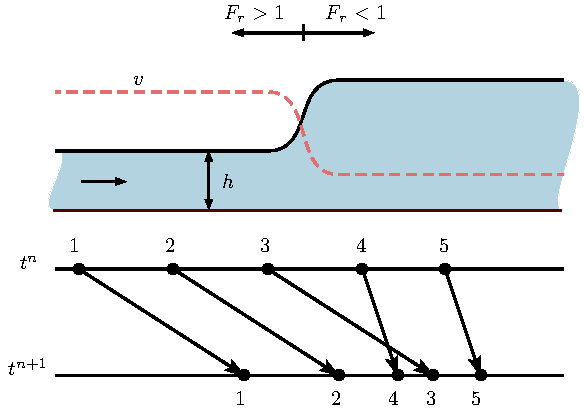
\includegraphics[width=.8\textwidth]{img/lagrangian/pfem_shock.pdf}
    \caption{Incompatibility of the mesh moving algorithm for solving problems with shocks.}
    \label{pfem_shock}
\end{figure}

While the primitive variables are not optimal to solve shocks, the mesh moving algorithm presents another difficulty.
Both methods present restrictions, but the nature of that difficulties are different. The restriction of the primitive variables is related to the conservation of the momentum at discrete level. The restriction of the mesh moving algorithm is associated to the finite differencing convective operator.





\section{Fixed mesh methods}


In this section a Lagrangian procedure with fixed mesh is presented. This procedure is an extension of PFEM-2 \cite{idelsohn2012} to the SW equations. In contrast to the mesh moving algorithm, the particles does not coincide with the nodes, but they move over the FE mesh. This procedure has the advantage of avoiding the remeshing step, but the cost of a projection from the particles to the mesh.

Let $\mathcal{P}$ be a set of particles randomly seed over the SW domain. The density of the particles is such that the average number of particles per element is greater than one. This particles move over the domain transporting the intrinsic variables of the fluid, namely density, water depth, flow rate, etc. This convection stage is finalized with a projection of the variables of the particles to the FE mesh.
The solution of the step is completed with the FE counterpart, solved in the fixed mesh following a Lagrangian framework. Finally, updating the particles is a trivial operation since the FE interpolation allows to evaluate the unknowns at an arbitrary point, namely, the particles.
Figure \ref{pfem2_stage_flowchart} summarizes the main stages of the PFEM-2 algorithm.


\begin{figure}
    \centering
    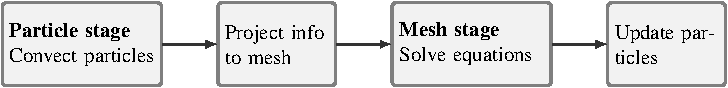
\includegraphics[width=\textwidth]{img/lagrangian/pfem2_stage_flowchart.pdf}
    \caption{PFEM-2 flowchart}
    \label{pfem2_stage_flowchart}
\end{figure}


In the same way as the mesh moving algorithm, this scheme may undergo certain variations. Strictly speaking, the mass and momentum balance are a coupled system of equations and the Lagrangian split does not modify that property. This will be analyzed in the following sections.



\subsection{Governing equations}


In contrast to the moving mesh algorithm, the nodes receive information from the particles without experimenting mesh displacement.
This fact allows to arbitrarily choose a Lagrangian or Eulerian framework, even for only one of the balance equations.
This property of the PFEM-2 algorithm allows more flexibility. The choose of the equations as well as the framework can optimize the computational cost and the approximation of the physical properties.
For example, Heniche pointed out in \cite{heniche2000} that the residual of the momentum balance does not distinguish the sign of the water depth if conservative variables are employed, $\mathbf{r}_\mathbf{q}(h) = \mathbf{r}_\mathbf{q}(-h)$.
This property suggests the use of conservative variables in combination with a mixed framework.
\begin{subequations} \label{pfem2_sw_eq}
\begin{align}
    &\frac{D\mathbf{q}}{Dt} + \mathbf{q} \nabla \cdot \mathbf{u} + gh \nabla (h-z) + S_f = \mathbf{0} \\
    &\pder{h}{t} + \nabla \cdot \mathbf{q} = 0
\end{align}
\end{subequations}


The first term involving spatial derivatives in the momentum balance comes from applying the chain rule to the fluxes vector and subtracting the convective term. The remaining terms corresponds to the compressibility of the SW equations --it is important to remember the analogy between the SW equations and the compressible NS equations--.

Several possibilities are presented to deal with this term. The first one consists on recovering the Eulerian quasi-linear form and then, apply the material derivative. The second one imply a projection to compute the divergence of the velocity. Lastly, an updated Lagrangian formulation can be used to compute the divergence term.

The first option is preferred since it is more consistent with the previous sections and does not introduce extra steps. The linearization matrices follow the next expression:
\begin{equation}
    \mathbf{A}_1 = \left[\begin{matrix}
        u_1  & 0   & -u_1^2 + gh \\
        u_2  & 0   & -u_1 u_2 \\
        1    & 0   & 0
    \end{matrix} \right]
    \quad , \quad
    \mathbf{A}_2 = \left[\begin{matrix}
        0   & u_1  & -u_1 u_2 \\
        0   & u_2  & -u_2^2 + gh \\
        0   & 1    & 0
    \end{matrix} \right]
\end{equation}




\subsection{PFEM-2 algorithm}


The outlined algorithm is explained in more detail in the section. The more important parts are the computations carried out by each discrete space. The communication between them and the integration in time are strictly related.


\subsubsection{Convection}


Let us assume that the particles move as material points and that each one stores the point concentration of the property $\phi_p = \phi(\mathbf x_p)$. Since the variables are not known for any arbitrary time $t$, but only for the discrete time steps $1,\ 2\dots n,\ n+1\dots$, the advection of a particle can be approximated using a $\theta$-family discretization as:
\begin{equation}
\mathbf{x}_p^{n+1} = \mathbf{x}_n^p + (1-\theta) \int_{t_n}^{t_{n+1}} \mathbf{v}_n(\mathbf{x}_p^t)dt + \theta \int_{t_n}^{t_{n+1}} \mathbf{v}_{n+1}(\mathbf{x}_p^t)dt
\end{equation}

If the velocity field is known, the system becomes explicit and the problem is reduced to moving the particles along the streamlines. The problem is solved using an explicit forward integration ($\theta=0$) with a proper sub-step \cite{idelsohn2012}. An illustration is given in figure \ref{pfem2_convection_stage}. This method, also known as XIVAS \cite{idelsohn2013}\cite{idelsohn2014}, was initially applied to a variable velocity field.
After the particles are moved, the ones that leave the domain are removed.

In this work the computational domain is initially seeded with fifteen particles per element. This number does not remain constant during the simulation because particles can freely enter and exit finite elements as they move through the domain. Thereby, in order to properly perform the advection stage, every time step the domain is reseed with particles so as to ensure that a minimum number is present within each finite element. This number of particles was chosen to be four. Particles can also be eliminated from each finite element in order to limit the computational cost. In this case, the maximum number of particles allowed per finite element is sixteen. These particle thresholds were chosen as they have proven to give accurate results in previous works \cite{idelsohn2015}.

\begin{figure} [htb]
\begin{subfigure}{0.48\textwidth}
    \centering
    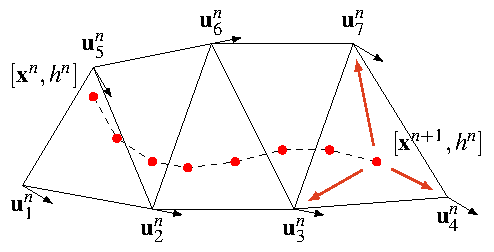
\includegraphics[width=\textwidth]{img/lagrangian/pfem2_convection_stage.pdf}
    \caption{Explicit advection stage using particles (in red). Next, the particles' information is transferred to the mesh nodes.}
    \label{pfem2_convection_stage}
\end{subfigure}
\hfill
\begin{subfigure}{0.48\textwidth}
    \centering
    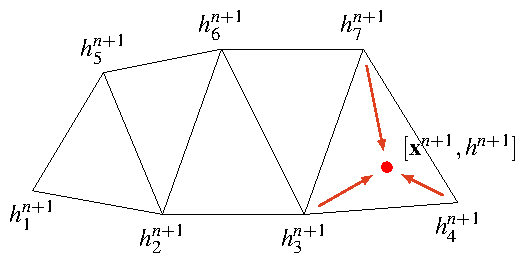
\includegraphics[width=\textwidth]{img/lagrangian/pfem2_wave_stage.pdf}
    \caption{After the computation of the wave stage, the FE nodes contribute to the particles.}
    \label{pfem2_wave_stage}
\end{subfigure}
\caption{Illustration of the two main steps of the PFEM2 framework.}
\label{pfem2_diffusion_and_wave_stages}
\end{figure}



\subsubsection{Projection}


When solving the advective stage in Equation (\ref{pfem2_sw_eq}), the particles concentration at $\mathbf x_p^{n+1}$ is the same as at the onset of the time step ($\mathbf x_p^n$). This is equivalent to saying that the advective step assumes $\frac{D\phi}{D t}=0$. This modification in the field described by the particles needs to be transferred onto the finite element space. As usual in particle-based techniques, such as PFEM, a projection procedure is used to transfer the information from the particles to the finite elements in the underlying mesh. In our work we use

\begin{equation}
    \phi^* = \mathcal L(\phi_p)
\end{equation}

where $\mathcal L$ is the projection operator from the particles to the finite element space and $\phi^*$ is the result of the advection at the time step $n+1$. In this case, a first order explicit projection has been used and all the particles in the elements surrounding a node contribute to that node, i.e.
%TODO: ($\theta = ? $)

\begin{equation}
    \phi_i^* = \dfrac
    {\Sigma_e\Sigma_{p_e} w_p \phi_p}
    {\Sigma_e\Sigma_{p_e} w_p}
    \quad \text{with} \quad
    w_p = N_{ei}(\mathbf x_p)
\end{equation}

where the index $i$ runs over all the mesh nodes, where $e$ runs over the elements sharing node $i$ and where $p_e$ runs over the particles contained in element $e$.


\begin{figure} [htb]
\begin{subfigure}{0.47\textwidth}
    \centering
    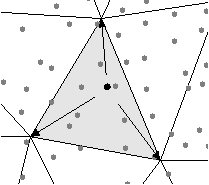
\includegraphics[width=\textwidth]{img/lagrangian/projection.pdf}
    \caption{Each particle contribute to the nodes from its element.}
    \label{pfem2_projection}
\end{subfigure}
\hfill
\begin{subfigure}{0.47\textwidth}
    \centering
    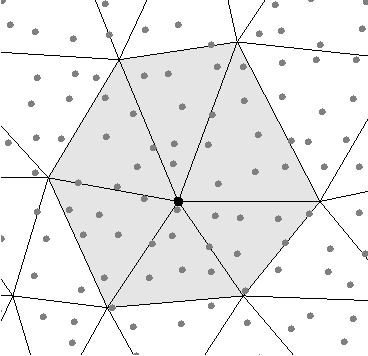
\includegraphics[width=\textwidth]{img/lagrangian/projection_full.pdf}
    \caption{Kernel of elements and particles contributing to a node.}
    \label{pfem2_projection_full}
\end{subfigure}
\caption{Illustration of the projection stage of the PFEM2 framework.}
\label{pfem2_projection_full_illustrations}
\end{figure}


\subsubsection{Wave equation stage}


Once the convective problem is solved explicitly in the particles and the results are transferred to the mesh nodes, the lagrangian residual (Equation (\ref{pfem2_sw_eq})) is solved in a fixed mesh with an Eulerian FIC-FEM technique. The spatial discretization and the time integration scheme follows the procedure explained in Section \ref{sec:fic_fem_stabilization}.
However, the time integration scheme follows a first-order BDF or Backward Euler.
The time derivatives are computed according to the next expressions
\begin{align} \label{pfem2_time_derivatives}
    \dot{\mathbf{q}} &= \frac{\mathbf{q}^{n+1} - \mathbf{q}^*}{\Delta t} \\
    \dot{h} &= \frac{h^{n+1} - h^n}{\Delta t}
\end{align}
Equation (\ref{pfem2_time_derivatives}) includes the contribution of the advection computed with the particles through the variables $^*$. It is important to note that the water depth is still using a partial derivative.

Another minor modification with respect to the Eulerian framework, is the use of the convected values as initial guess for the iterative strategy:
\begin{align}
    \mathbf{q}^{n+1,0} = \mathbf{q}^* \\
    h^{n+1,0} = h^*
\end{align}

Finally, it is worth to remark the need of stabilization, since the discretization does not fulfill the compatibility of interpolation. Though, several authors report instabilities but does not associate them to the \emph{inf-sup} condition. The stability is introduced following the procedure explained in section \ref{sec:fic_fem_stabilization}.


\subsubsection{Particles update}
The last step of the PFEM2 algorithm is to add the contribution of the solution of Equation (\ref{pfem2_sw_eq}) to the particles. To avoid the accumulation of projection errors and additional diffusion, the information from the particles is updated using an incremental scheme. This step only involves the evaluation of the unknown at each particle position in the finite element mesh as:

\begin{equation}
    \phi_p^{n+1} = \phi_p^n + \phi({\bf x}_p^{n+1}) - \phi({\bf x}_p^*)
\end{equation}



\section{Examples}


In this section an example is presented as a proof of concept of the Lagrangian methods. Its advantages and drawbacks compared to the Eulerian framework are discussed. Here, the example presented in section \ref{sec:examples:parabola} is taken up again, since the oscillation benchmark is a good option to test the accuracy of the shoreline tracking.

As a reminder, this benchmark has been extracted from \cite{delestre2013} and has an analytical solution. The problem consists on a 1D parabolic basin containing a mass of water. The initial condition is zero velocity and the free surface describing an inclined plane. After the initial time $t=0$, the mass of water begins to slice over the parabolic basin and describes an oscillatory movement. The topography is described in equation (\ref{eq:parabola:topography}) and the analytical solution follows equation (\ref{eq:parabola:variables}). The same parameters than the ones in section \ref{sec:examples:parabola} are used in this example:
\begin{equation*}
    h_0 = 1 \quad,\quad a = 1
\end{equation*}

The spatial domain is $\Omega=[0,10]\times[0,1]m^2$, where the parabola is aligned with the larges dimension. 
Figure \ref{fig:pfem_parabola_view} shows the discretization of the problem using the PFEM algorithm. For visualization purpose, the meshes are deformed vertically with the topography and the free surface respectively.

\begin{figure}
    \centering
    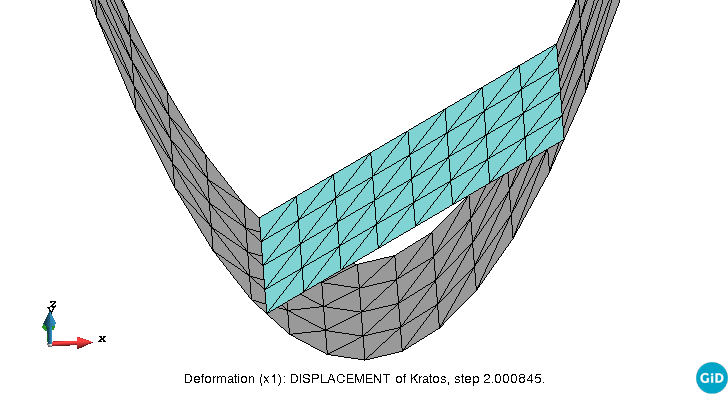
\includegraphics[width=.8\textwidth]{img/lagrangian/parabola_view.png}
    \caption{Detail of the discretizations used to solve the oscillation in a parabolic basin with the mesh moving algorithm (PFEM).}
    \label{fig:pfem_parabola_view}
\end{figure}



\begin{figure}
    \centering
    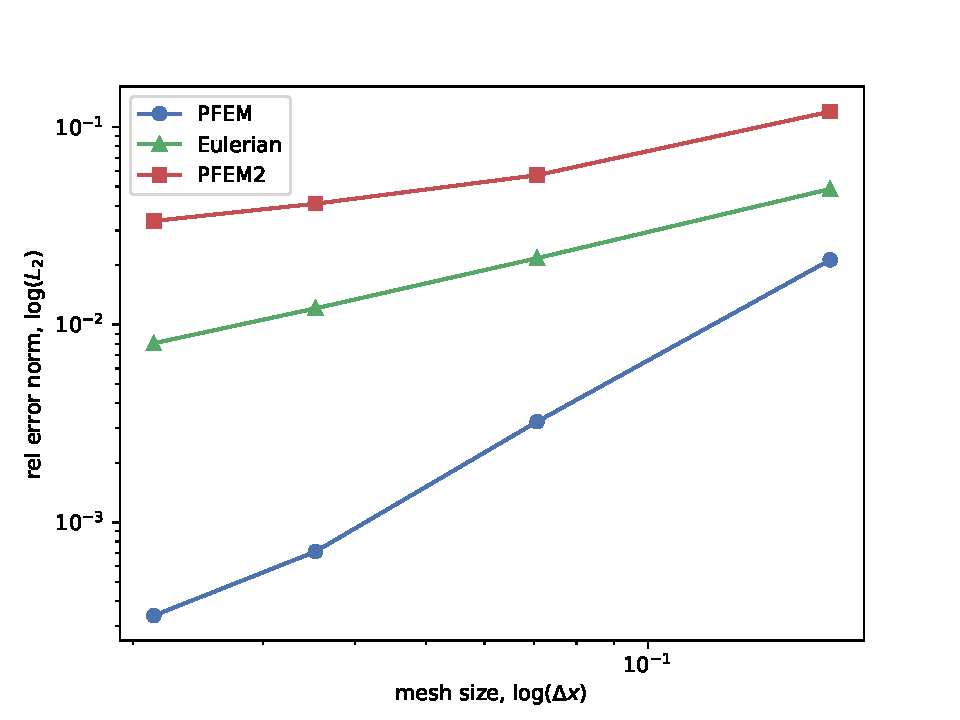
\includegraphics[width=.7\textwidth]{img/lagrangian/convergence}
    \caption{Comparison of the convergence for the presented methods.}
    \label{fig:lagrangian_parabola_convergence}
\end{figure}


A convergence analysis has been carried out with the proposed method and the results are summarized in Figure \ref{fig:lagrangian_parabola_convergence}. As expected, the order of convergence of the PFEM method is not affected by the moving shoreline, keeping the second order of the FE formulation.





\section{Concluding remarks}


Lagrangian methods exhibit some computational benefits but the main advantage is its natural tracking of the shoreline. Especially the mesh moving algorithm, does not need additional treatment since it is not affected by the dry domain. The main drawback of the Lagrangian methods is related to the compressible behavior of the SW equations. On the on side, the velocity field is discontinuous around shocks and the staggered character of the time strategy is not suited to this phenomena. Furthermore, the explicit calculation of the convection faces a strong restriction on the CFL number.
On the other side, the Lagrangian formulation does not achieve the desired linearization when compressible formulations are considered.
Figure \ref{pfem_euler_convergence} shows a schematic of the order of convergence in terms of the Froude number. When the Froude number is equal to 1, there is a discontinuity. The moving shoreline is characterized by a very elevated Froude number, since the shoreline involves a quasi zero water depth.

\begin{figure}
    \centering
    \includegraphics[width=\textwidth]{img/lagrangian/pfem_euler_convergence.png}
    \caption{Qualitative representation of the order of convergence in terms of the Froude number.}
    \label{pfem_euler_convergence}
\end{figure}


A global overview of the Lagrangian and Eulerian methods identifies the Eulerian framework as the robust one. Nevertheless, the Lagrangian framework is still interesting for the shoreline tracking.
A promising combination would be an arbitrary Lagrangian-Eulerian formulation using the Eulerian framework where shocks and oscillatory behavior is dominant, and using a Lagrangian framework where the shoreline is moving.



\chapter{Hierarchical mesh refinement with local time step}
\label{mesh_refinement}


Keeping the time step under a certain value relative to the element size in transitory problems is of key importance to achieve good results. Otherwise, an excessively large time step could resort on an over-diffusive solution.
Furthermore, the element size is governed by the physics, it has to be small enough to capture the modes of interest. It is a usual practice to refine the mesh near the region of interest or where the solution is changing rapidly. consequently, the local reduction of the mesh size is imposing a global reduction of the time step.

This section seeks for a strategy with local tie step. The main idea consists on the division on subdomains characterized by its mesh size. Thus, a hierarchic mesh refinement is defined with a characteristic mesh size and the corresponding time step. The hierarchical refinement allows to use both non-conforming discretization at space and at time level. The only requirement is having a natural number of divisions in order to perform a communication at the coarse level. Figure \ref{multigrid_refinement} shows a hierarchical spatial refinement.

This framework eases the refinement and coarsening procedures. Specially simple is the coarsening process, since it consists just on removing elements from a lower level without having to rebuild the connectivities. On the other hand, a procedure must be defined for the hanging nodes at the boundary and the hanging time steps.



\begin{figure}
\centering
\begin{subfigure}{.8\textwidth}
    \includegraphics[width=\textwidth]{img/multigrid/grid1.pdf}
    \vspace{1em}
\end{subfigure}
\begin{subfigure}{.8\textwidth}
    \includegraphics[width=\textwidth]{img/multigrid/grid2.pdf}
    \vspace{1em}
\end{subfigure}
\begin{subfigure}{.8\textwidth}
    \includegraphics[width=\textwidth]{img/multigrid/grid3.pdf}
    \vspace{1em}
\end{subfigure}
\caption{Different refinement zones for a domain.}
\label{multigrid_refinement}
\end{figure}



\section{Algorithm}


\begin{figure}
    \centering
    \includegraphics[width=.8\textwidth]{img/multigrid/multigrid_steps.png}
    \caption{Steps for solving a coarse time step with hierarchical refinement.}
    \label{multigrid_steps}
\end{figure}


\section{Data structure}


\section{Refinement criterion}


\section{Examples}





\chapter{Search algorithm}
\label{search_algorithm}



Usually, Lagrangian frameworks involve the computation of the streamlines or projections. The computation of the streamlines is related to the material derivative and is part of the differentiation. The projections are part of the communication between the Lagrangian and Eulerian domains, and belong to the numerical environment. Those task require the search of material points (streamlines) or nodes (projections) over the spatial discretization. This happens both in the fixed mesh PFEM-2 algorithm or in the mesh moving PFEM algorithm. As counterpart to the simplicity in the system computation provided by the Lagrangian algorithms, a search algorithm is required.

In this appendix, the search algorithm used and implemented for the presented work is explained. It is based on the \emph{divide and conquer} strategy. The main domain is firstly partitioned using a dynamic bins structure, a detailed explanation can be found in \textcolor{red}{[............]}. In brief, the dynamic bins are a search structure where the cell size is higher than the characteristic element size. 

\begin{figure}
    \centering
    \includegraphics[width=.9\textwidth]{img/search/bins_search.pdf}
    \caption{Left: Mesh and point to locate in the mesh. Right: Mesh and point with the search structure}
    \label{bins_search}
\end{figure}

%El algoritmo de búsqueda se basa en una estructura dinámica bins, explicada con detalle en \textcolor{red}{[............]}. De modo resumico, entre el nodo o entidad a buscar y la malla, se interpone una estructura de búsqueda, que consiste en una partición regular del dominio, definida por un tamaño de celda.

Esta estructura de búsqueda tiene un coste inicial de creación, pero luego, ahorra enormemente el tiempo de búsqueda. En primer lugar, la estructura de búsqueda consiste en la definición de las celdas. En segundo lugar, se realiza una búsqueda entidad a entidad para asociar los elementos intersectados por una celda con ella. La comparación de elementos con celdas podría hacerse mediante proyecciones, sin embargo se ha empleado el método descrito por Möller \cite{moller2004}, que se describe más abajo.

Una vez definida la estructura de búsqueda, el proceso de búsqueda también tiene dos pasos. En primer lugar, se determina en qué celda cae el nodo o partícula en cuestión. Nótese que esta búsqueda es trivial y puede hacerse en paralelo. El resultado será una lista de elementos candidatos. En segundo lugar, se realiza otra búsqueda, más costosa, pero solamente en un número reducido de candidatos. Esta segunda búsqueda requiere hacer una comprobación punto-elemento, que involucra la evaluación de las funciones de forma o bien, el cálculo de proyecciones.



\section{Triangle vs aligned box intersection}

La explicación completa puede encontrarse en \cite{moller2004}. Si bien el problema podría reducirse a un caso 2D, se ha desarrollado la versión genérica 3D, por su extensibilidad a las ecuaciones de convección-difusión, Navier-Stokes u otros problemas. La adaptació al caso bidimensional es trivial y se explicará en este anexo.

La derivación de este algoritmo se basa en el \emph{Separating Axis Theorem} \cite{gottschalk1996}. Consiste en una búsqueda de separating axis entre los dos objetos. La figura \ref{triangle_aabb} muestra los 13 ejes posibles (los tres ejes cartesianos $\mathbf{e}_i$, el vector normal $\mathbf{n}$ y las cominaciones entre los ejes $\mathbf{f}_j$ con $\mathbf{e}_i$). Cuando un test halla un separating axis, el algoritmo de detiene y el resultado es que no hay intersección. Si hay intersección, se ejecutarán todos los test, pues ninguno encontrará un separating axis.

De acuerdo con la Figura \ref{triangle_aabb}, la primera operacion consiste en trasladar el triángulo de modo que el AABB quede centrado en el origen de coordenadas. Los tests a pasar son:

\begin{figure}
\centering
\includegraphics[width=.6\textwidth]{img/search/triangle_aabb.pdf}
\caption{Notación empleada para buscar un separating axis entre triángulo y AABB}
\label{triangle_aabb}
\end{figure}

\begin{description}
    \item[Ejes cartesianos] (3 tests) El primer set de tests consiste en comparar en las tres direcciones $\mathbf{e}_i$ el AABB respecto el mínimo AABB del triángulo. En pseudocódigo la búsqueda de un separating axis queda:
    \begin{verbatim}
for i = 0:2
    min, max = min_max(triangle_points)
    if (min > half_box_size or max < -half_box_size)
        return true
return false
    \end{verbatim} 
    \item[Vector normal] (1 test) El segundo conjunto de tests consiste en una comparación AABB - plano. Para ello se define el plano que contiene el triángulo com el vector normal $\mathbf{n}$ y la distancia a origen $d$. La búsqueda de un separating axis se realiza en el mismo octante que el vector $\mathbf{n}$, de modo análogo al test anterior.
    \item[Aristas] (9 tests) Se realiza un test por cada combinación $\mathbf{a}_{ij} = \mathbf{n}_i \times \mathbf{f}_j$. Cada test supone hacer una proyección del triángulo y el AABB, la comparación se realiza siguiendo el algoritmo del primer test. Afortunadamente, el desarrollo de las proyecciones presenta algunas simplificaciones. Para la primera proyeccion tenemos:
    \begin{align*}
        p_0 &= \mathbf{a}_{00} \cdot \mathbf{v}_0 = (0, -f_{0z}, f_{0,y}) \cdot \mathbf{v}_0 = v_{0z}v_{1y} - v_{0y}v_{1z} \\
        p_1 &= \mathbf{a}_{00} \cdot \mathbf{v}_1 = (0, -f_{0z}, f_{0,y}) \cdot \mathbf{v}_1 = v_{0z}v_{1y} - v_{0y}v_{1z} = p_0 \\
        p_2 &= \mathbf{a}_{00} \cdot \mathbf{v}_2 = (0, -f_{0z}, f_{0,y}) \cdot \mathbf{v}_2 = (v_{1y} - v_{0y}) v_{2z} - (v_{1z} - v_{0z}) v_{2y}
    \end{align*}
    El hecho de que $p_0 = p_1$ facilita la búsqueda del máximo y mínimo de $p_0$, $p_1$ y $p_2$. Éstos se tiene que comparar con el "radio" de la caja, que es la proyección de una esquina sobre $\mathbf{a}_{00}$:
    \begin{align*}
        r = h_x |a_{00x}| + h_y |a_{00y}| + h_z |a_{00z}|
    \end{align*}
    Finalmente, la búsqueda de un separating axis consiste en:
    \begin{verbatim}
        if (min(p0, p2) > r or max(p0, p2) < -r)
            return true
    \end{verbatim}
\end{description}
Si todos los 13 tests descritos devuelven falso, significa que no hay ningún separating axis, e decir, hay intersección entre las dos geometrías. Nótese que solo con que un test de verdadero, el algoritmo se detiene, pues no habrá intersección posible.

\subsection{Particularización para 2D}

El caso bidimensional es una simplificacion del algoritmo general y algunos tests se pueden omitir. En total, se realizan 5 tests:
\begin{description}
    \item[Ejes cartesianos] Se busca un separating axis en $x$ e $y$.
    \item[Vector normal] Se omite.
    \item[Aristas] Solamente son relevantes las proyecciones de las aristas $\mathbf{f}_j$ con el eje $\mathbf{e}_z$.  
\end{description}



\section{Quadrilateral vs aligned box intersection}

El presente algoritmo es fácilmente extrapolable a cuadriláteros. Hay que modificar los tests de las aristas, por un lado, se incluye una arista nueva, por otro lado, cada test requiere de más condicionales, ya que hay un nodo adicional.

Sin embargo, se ha optado por dividir cada cuadrilátero en dos triángulos y realizar dos comprobaciones. Aunque el número de comprobaciones es significativamente mayor, esto supone un ahorro de código y de mantenimiento. El hecho de tomar esta aproximación es que no estamos interesados en la optimización del código, sino en la evaluación del métodos FEM.



\section{Point intersection}

Determinar si un punto está dentro de un triángulo lineal o cuadrilátero bilineal es una operación sencilla. Tan solo es preciso determinar el punto en coordenadas locales y verificar si todas ellas estan entre 0 y 1 en el caso de un triángulo. Entre -1 y 1 en el caso de cuadriláteros. De modo equivalente y para elementos linales o bilineales, esta comprobación se puede expresar en términos de las funciones de forma, permite ahorrar la evaluación de condicionales:
\begin{verbatim}
function is_inside
    for i = 1 : n_nodes
        if N(i) < 0
            return false
    return true
\end{verbatim}






%----------------------------------------------------------------------------------------
%	BIBLIOGRAPHY
%----------------------------------------------------------------------------------------

\printbibliography[heading=bibintoc]

%----------------------------------------------------------------------------------------

\end{document}  
